\documentclass[acmsmall,screen]{acmart} 


\acmConference[OOPSLA '19]{Proceedings of the ACM on Programming Languages, Volume 3, Number OOPSLA}{October 20–25, 2019}{Athens, Greece}
\acmYear{2019}
\acmISBN{} \acmDOI{} \startPage{1}

\setcopyright{acmcopyright}


\bibliographystyle{ACM-Reference-Format}
\citestyle{acmauthoryear}  






\usepackage{listings}          \usepackage{stmaryrd}          \usepackage{mathtools}         \usepackage{semantic}          \usepackage{mathpartir}        \usepackage{tikz}              \usepackage{courier}           \usepackage{multicol}          \usepackage{subcaption}        \usepackage[export]{adjustbox} \usepackage{accents}
\usepackage{wrapfig}
\usepackage{scalerel}
\usepackage{graphicx}
\usepackage{fvextra}

\renewcommand*{\ttdefault}{zi4}

\makeatletter
\newlength{\@mli}
\newcommand{\mli}[1]{\settowidth{\@mli}{\lstinline/#1/}
  \hspace{-.5ex}\begin{minipage}[t]{\@mli}\lstinline/#1/\end{minipage}}
\newcommand{\ostar}{\mathbin{\mathpalette\make@circled\ast}}
\newcommand{\make@circled}[2]{\ooalign{$\m@th#1\smallbigcirc{#1}$\cr\hidewidth$\m@th#1#2$\hidewidth\cr}}
\newcommand{\smallbigcirc}[1]{\vcenter{\hbox{\scalebox{0.66667}{$\m@th#1\bigcirc$}}}}
\makeatother

\newcommand{\li}[1]{{\texttt{\small #1}}}
\newcommand\hide[1]{}
\newcommand{\MV}{\ensuremath{\mathsf{ModVar}}}
\newcommand{\FV}{\ensuremath{\mathsf{FreeVar}}}
\newcommand{\pguards}[1]{\llbracket #1 \rrbracket}
\newcommand{\reachable}[5]{\ensuremath{{\m{#1}\;\accentset{#2}{\leadsto}^{#3}_{#4} \m{#5}}}}

\newcommand{\minbar}{\scalebox{1.0}[1.0]{$-$}}
\newcommand{\scon}{\mathbin{\star}}
\renewcommand{\scon}{\mathbin{\ast}} \renewcommand{\bigstar}{\raisebox{-0.24em}{{\scaleobj{2.5}{\scon}}}}
\newcommand{\ocon}{
  \mathbin{\mbox{$\mathrlap{\cup}\hspace*{.09em}
      \raisebox{.04em}[0ex][0ex]{$\scon$}$\hspace*{.07em}}}}
\newcommand{\bigocon}{\raisebox{-0.3ex}{\resizebox{0.75em}{!}{\hspace{0.05em}$\scon$}}\hspace{-2.18ex} \bigcup}
\newcommand{\wand}{\mathrel{\mbox{$\hspace*{-0.03em}\mathord{-}\hspace*{-0.4em}
  \mathord{-}\hspace*{-0.13em}
     \mathord{\scon}$\hspace*{-0.005em}}}}
\newcommand{\septraction}{\mathrel{\mbox{$\hspace*{-0.03em}\mathord{-}\hspace*{-0.66em}
  \mathord{-}\hspace*{-0.1em}\mathord{\ostar}$\hspace*{0.05em}}}}
\colorlet{red}{red!80!black}
\colorlet{lightgray}{gray!20!white}
\newcommand{\vdashtwo}{\vdash\hspace*{-0.5em}\mathord{-}}
\newcommand{\finf}{finf}
\newcommand{\tinf}{tinf}
\newcommand{\out}{out}
\newcommand{\braces}[1]{\left\{\!\!\!\begin{array}{l@{}} #1 \end{array}\right\}}
\newcommand{\ga}{\gamma}
\newcommand{\Eg}{E_\ga}
\newcommand{\Vg}{V_\ga}

\let\magicwand\wand
\let\emptyset\varnothing
\mathlig{--*}{\mathrel{\magicwand}}
\mathlig{--o}{\mathrel{\septraction}}
\mathlig{|->}{\mathrel{\mapsto}} \mathlig{<=>}{\mathrel{\Leftrightarrow}} \mathlig{==>}{\mathrel{\Rightarrow}} \mathlig{-|-}{\mathrel{\mathrlap{\dashv} \hspace*{0.15em} \vdash}} \mathlig{**}{\mathbin{\ocon}}
\mathlig{*}{\mathbin{\scon}}
\mathlig{/|}{\mathbin{\wedge}} \mathlig{|/}{\mathbin{\vee}} \mathlig{|-}{\mathrel{\vdashtwo}} \mathlig{|=}{\models} \mathlig{//}{\color{black}{\sslash}} 

\newcommand{\defeq}{\mathbin{\stackrel{\triangle}{=}}}
\newcommand{\tx}[1]{\text{#1}}
\newcommand{\p}[1]{\ensuremath{\mathsf{#1}}} \newcommand{\m}[1]{\ensuremath{\mathit{#1}}} \newcommand{\ma}[1]{\ensuremath{\mathcal{#1}}} \let\ramify\lightning
\newcommand{\infrulestyle}[1]{\textsc{#1}}
\newcommand{\infrule}[4]{\inferrule*[lab=\infrulestyle{#1},right=$\mathrlap{#4}$]{#2}{#3}}
\newcommand{\medocon}{
  \raisebox{-0.3ex}{\resizebox{0.63em}{!}{$\scon$}} \hspace{-2.05ex} \bigcup}
\newcommand{\triple}[3]{\{#1\}\,#2\,\{#3\}}
\newcommand{\hl}[1]{\colorbox{lightgray}{#1}}

\lstset{language=C,
morecomment=[l][{\color{red}}]{//},
  sensitive=true, mathescape=true, showlines=true, escapechar=`,
  basicstyle=\footnotesize\ttfamily,
  keywordstyle=\color{blue}, numbers=left,
  numberstyle=\tiny, numbersep=5pt, boxpos=t,
  showstringspaces=false
}
\usetikzlibrary{arrows.meta, positioning, decorations.pathmorphing, fit}

\begin{document}

\title[Certifying Graph-Manipulating Programs]
{Certifying Graph-Manipulating C Programs via~Localizations within Data Structures}





\author[S. Wang]{Shengyi Wang}
\affiliation{
\institution{National University of Singapore} }


\author[Q. Cao]{Qinxiang Cao}
\affiliation{\institution{Shanghai Jiao Tong University}}


\author[A. Mohan]{Anshuman Mohan}
\affiliation{\institution{National University of Singapore}}


\author[A. Hobor]{Aquinas Hobor}
\affiliation{\department{blah}\department{bloop}\institution{National University of Singapore}}



\hide{
\author{First2 Last2}
\authornote{with author2 note}          \orcid{nnnn-nnnn-nnnn-nnnn}             \affiliation{
  \position{Position2a}
  \department{Department2a}             \institution{Institution2a}           \streetaddress{Street2a Address2a}
  \city{City2a}
  \state{State2a}
  \postcode{Post-Code2a}
  \country{Country2a}                   }
\email{first2.last2@inst2a.com}         \affiliation{
  \position{Position2b}
  \department{Department2b}             \institution{Institution2b}           \streetaddress{Street3b Address2b}
  \city{City2b}
  \state{State2b}
  \postcode{Post-Code2b}
  \country{Country2b}                   }
\email{first2.last2@inst2b.org}         } 

\begin{abstract}
We develop powerful and general techniques to mechanically verify realistic programs that
manipulate heap-represented graphs.  These graphs can exhibit well-known organization 
principles, such as being a directed acyclic graph or a disjoint-forest; alternatively, these graphs can 
be totally unstructured.  The common thread for such structures is that they exhibit deep 
intrinsic sharing and can be expressed using the language of graph theory. 
We construct a modular and general setup for reasoning about abstract mathematical
graphs and use separation logic to define how such abstract graphs are represented concretely in
the heap. We develop a \infrulestyle{Localize} rule that enables modular reasoning
about such programs, and show how this rule can support existential
quantifiers in postconditions and smoothly handle modified program variables.
We demonstrate the generality and power of our techniques by integrating them into 
the Verified Software Toolchain and certifying the correctness of seven graph-manipulating 
programs written in CompCert C, including
a 400-line generational garbage collector for the CertiCoq project.
While doing so, we identify
two places where the semantics of C is too weak to define generational
garbage collectors of the
sort used in the OCaml runtime.  Our proofs are entirely machine-checked in Coq.
\end{abstract}

\begin{CCSXML}
<ccs2012>
<concept>
<concept_id>10003752.10003790.10011742</concept_id>
<concept_desc>Theory of computation~Separation logic</concept_desc>
<concept_significance>500</concept_significance>
</concept>
<concept>
<concept_id>10003752.10010124.10010138.10010142</concept_id>
<concept_desc>Theory of computation~Program verification</concept_desc>
<concept_significance>500</concept_significance>
</concept>
<concept>
<concept_id>10003752.10003790.10002990</concept_id>
<concept_desc>Theory of computation~Logic and verification</concept_desc>
<concept_significance>300</concept_significance>
</concept>
<concept>
<concept_id>10003752.10010124.10010138.10010140</concept_id>
<concept_desc>Theory of computation~Program specifications</concept_desc>
<concept_significance>100</concept_significance>
</concept>
</ccs2012>
\end{CCSXML}

\ccsdesc[500]{Theory of computation~Separation logic}
\ccsdesc[500]{Theory of computation~Program verification}
\ccsdesc[300]{Theory of computation~Logic and verification}
\ccsdesc[100]{Theory of computation~Program specifications}




\keywords{Separation logic, Graph-manipulating programs, Coq, CompCert, VST}  


\maketitle

\section{Introduction}
\label{dummyref} \label{sec:intro}
Over the last fifteen years, separation logic has facilitated great strides
in verifying programs that manipulate tree-shaped data structures.
\citep{berdine:smallfoot,chin:hipsleek,jacobs:verifast,
chlipala:bedrock,bengtson:charge,appel:programlogics}.
Unfortunately, programs that manipulate graph-shaped data structures
(\emph{i.e.} structures with \emph{intrinsic sharing}) have proved harder to verify.
Indeed, such programs were formidable enough that many of the early
landmark results in separation logic devoted substantial effort to verifying
single examples such as Schorr-Waite~\cite{hongseok:phd} or
union-find~\cite{neelthesis} with pen and paper.
More recent landmarks have moved to a machine-checked context, but have still
been devoted to either single examples or to classes of closely-related examples
such as garbage collectors~\cite{gcexample3,cakemlgc}.
These kinds of examples tend to require a large number
of custom predicates and subtle reasoning, which generally
does not carry over
to the verification of other graph-manipulating programs.

In contrast, we present a toolkit for verifying graph-manipulating programs in a
machine-checked context. Our techniques are \emph{general} in that they handle a diverse
range of programs, and \emph{modular} in that they encourage code
reuse (\emph{e.g.} facts about reachability) and separation of concerns
(\emph{e.g.} between abstract mathematical graphs and concrete representations
in the heap).
Our techniques are \emph{powerful} enough to reason about real C code as compiled by
CompCert~\cite{leroy:compcert}, and also
\emph{lightweight} enough to integrate into the Verified
Software Toolchain (VST)~\cite{appel:programlogics} without major reengineering.
CompCert and VST are distributed via opam and the CoqIDE installer, so they have a sizable userbase that can take advantage of our techniques. Finally, our techniques \emph{scale} well beyond short toy programs: we certify the
correctness of a generational garbage collector for the CertiCoq
project~\cite{certicoqpaper} ($\approx400$ rather devilish lines of C).

We proceed in three steps. First, we develop a mathematical graph library that is general enough to reason about a wide variety of algorithms and expressive enough to describe the behavior of these algorithms in real machines.  We modularize this library carefully so that common ideas---\emph{e.g.}~subgraphs, reachability, and isomorphism---can be efficiently reused
in different algorithms.  Second, we use separation logic to express how these abstract graphs
are actualized in the heap as concrete graphs in a way that facilitates the reuse of key definitions and theorems across algorithms.  Third, we develop a notion of \emph{localization blocks} that
enables modular reasoning in our Hoare proofs, even in the presence of the
implicit sharing intrinsic to graphs, by using our \textsc{Localize} rule:

\hide{
\begin{equation}
\label{eq:localize}
\begin{array}{@{}l@{}}
\infrule{Localize}
{G_1 |- L_1 * R \\
\{ L_1 \} ~ c ~ \{ \exists x.~ L_2 \} \\
R |- \forall x.~ (L_2 --* G_2) }
{\{ G_1 \} ~ c ~ \{ \exists x.~ G_2 \}} {(\dagger)} \\
[3pt]
(\dagger)~ \mathit{freevars}(R) \cap \MV(c) = \emptyset
\end{array}
\end{equation} \marginpar{Can we typeset this a little better?}
} 
\vspace{-1em}
\begin{equation}
\label{eq:localize}
\inferrule[Localize]	
{G_1 |- L_1 * R \\
\{ L_1 \} ~ c ~ \{ \exists x.~ L_2 \} \\
R |- \forall x.~ (L_2 --* G_2) }
{\{ G_1 \} ~ c ~ \{ \exists x.~ G_2 \}} \; \FV(R) \cap \MV(c) = \emptyset \qquad
\vspace{-0.3em}
\end{equation}
\textsc{Localize} connects the ``local'' effect of a command~$c$, \emph{i.e.}
transforming~$L_1$ to~$L_2$, with its ``global'' effect, \emph{i.e.} from~$G_1$ to~$G_2$.
\textsc{Localize} is a more general version of the well-known \textsc{Frame} rule,
which does the same task in the simpler case when $G_i = L_i * F$
for some frame~$F$ that is untouched by~$c$.
\textsc{Localize} can handle the more general transformation if we can find a \emph{ramification frame}~$R$ that satisfies a pair of
delicately-stated entailments\footnote{Readers less familiar with the separating implication $P --* Q$, also known as \emph{magic wand}, can refer to its semantics in Figure~\ref{fig:seplogsem} (page~\pageref{fig:seplogsem}), which also models the other separation logic operators
we use in this paper.  The key proof rule for magic wand is its adjointness
with the separating conjunction:~$(P * Q |- R) \Leftrightarrow (P |- Q --* R)$.} and
the side condition on modified local program variables.
\textsc{Localize} upgrades the \textsc{Ramify} rule~\cite{hobor:ramification} in two key ways:
support for existential
quantifiers in postconditions and smoother treatment of modified program variables.


Our contributions are organized as follows:
\begin{itemize}
\item[\S\ref{sec:orientation}] We use the classic ``union-find'' disjoint set algorithm to show how our three key ingredients---mathematical graphs, spatial graphs, and localization blocks---come together to verify
graph-manipulating algorithms.
To the best of our knowledge this is the first machine-checked verification of this algorithm that starts with real C code.
We briefly review the seven programs we have already verified to give a sense 
of the breadth of algorithms our system can tackle.
\item[\S\ref{sec:localizations}] We show that \textsc{Localize} and \textsc{Frame} are co-derivable.  We illustrate a delicate technique to properly handle modified 
local variables. We show a mark-graph
program that explores a graph in a fold/unfold style, and discuss the utility of linked
existentials in postconditions.  

\item[\S\ref{sec:mathgraph}] We develop a general and modular framework of mathematical graphs powerful enough to support realistic verification in a mechanized context.  We give a sampling of key definitions.
\item[\S\ref{sec:spacegraph}] We suggest that the Knaster-Tarski fixpoint~\cite{tarski:fixpoint} cannot define a usable separation logic graph predicate.  We propose a better definition for general spatial graphs that still enjoys a ``recursive'' fold/unfold.  We prove general theorems about spatial graphs that are 
organized in a modular way that can be utilized in multiple flavors of separation logic. \item[\S\ref{sec:certigc}] We discuss our flagship example, the certification of the CertiCoq garbage collector (GC). We identify two places where the semantics of C is too weak to define an OCaml-style GC. We also find and fix a rather subtle overflow error in the original C code for the GC, thereby justifying the effort of developing machine-checked proofs of correctness.
\item[\S\ref{sec:development}] We discuss how our techniques are integrated into the
``Floyd'' module of VST, a separation-logic based engine to help users verify
CompCert~C programs, via two new Floyd tactics \li{localize} and \li{unlocalize}.
We also document statistics related to our overall development.
\item[\S\ref{sec:related}] We discuss related work.
\item[\S\ref{sec:conclusion}] We discuss directions for future work and conclude.
\end{itemize}
All of our results are machine checked in Coq and are available as an artifact online.
A version of this paper featuring three additional appendices is available 
at \href{www.example.com}{www.example.com}.
 
\section{Tour of a verified example}
\label{sec:orientation}
Before jumping into an involved discussion of our three-part recipe, 
we first~(\S\ref{sec:unionfind}) build intuition by showing how 
they are applied to verify a well-known algorithm. 
We then~(\S\ref{sec:localblocks}) explain our new \emph{localization blocks}. 
Finally~(\S\ref{sec:application}), we briefly discuss the other 
examples we have verified. 



\subsection{Localizations Yield a Tidy Union-Find}
\label{sec:unionfind}

\renewcommand{\tx}[1]{\scriptsize {\text{#1}}}

\begin{figure}[t]
\vspace{-1ex}
  \begin{lstlisting}[multicols=2]
`\hl{struct Node \{ unsigned int rank;}`
            `\hl{struct Node * parent; \}}`
$//$$\label{code:findstart}\{\p{uf\_graph}(\gamma) /| \tx{x}\in\m{V}(\gamma)\}$
`\hl{struct Node* find(struct Node* x) \{}`
  `\hl{struct Node *p;}`
$//$$\label{code:ufbefram1}\left\{\!\!\!\begin{array}{l@{}} \p{uf\_graph}(\gamma) /| \tx{x}\in\m{V}(\gamma) /| \null \\ {\color{red}\exists\m{r},\m{pa}.~\gamma(\tx{x}) = (\m{r}, \m{pa})} /| {\color{red}\m{pa}\in\m{V}(\gamma)} \end{array} \right\}$
$//$$\label{code:befparentfind} \searrow \left\{\!\!\!\begin{array}{l@{}} {\color{red}\tx{x}|-> \m{r},\m{pa}} /| \tx{x}\in\m{V}(\gamma) /| \null \\ \gamma(\tx{x}) = (\m{r}, \m{pa}) /| \m{pa}\in\m{V}(\gamma) \end{array}\right\}$
$\ramify(\ref{findram1})$  `\hl{p = x -> parent;}` $\label{code:findram1}$
$//$$\label{code:aftparentfind} \swarrow \left\{\!\!\!\begin{array}{l@{}} \tx{x}|-> \m{r},\m{pa} /| {\color{red}\tx{p} = \m{pa}} /| \tx{x}\in\m{V}(\gamma) /| \null \\ \gamma(\tx{x}) = (\m{r}, \m{pa}) /| \m{pa}\in\m{V}(\gamma)\end{array}\right\}$
$//$$\label{code:ufaftram1}\left\{\!\!\!\begin{array}{l@{}} {\color{red}\p{uf\_graph}(\gamma)} /| \tx{p} = \m{pa} /| \tx{x}\in\m{V}(\gamma) /| \null \\ \gamma(\tx{x}) = (\m{r}, \m{pa}) /| \m{pa}\in\m{V}(\gamma)\end{array}\right\}$
  `\hl{if (p != x) \{}` $\label{code:ufif}$
$//$$\label{code:ufaftpxeqcheck}\left\{\!\!\!\begin{array}{l@{}} \p{uf\_graph}(\gamma) /| \tx{p} = \m{pa} /| {\color{red}\m{pa} \neq \tx{x}} /| \null \\ \tx{x}\in\m{V}(\gamma) /| \gamma(\tx{x}) = (\m{r}, \m{pa}) /| \m{pa}\in\m{V}(\gamma)\end{array}\right\}$
    `\hl{p = find(p);}` $\label{code:ufreccall}$
$//$$\label{code:ufbefram2}\left\{\!\!\!\begin{array}{l@{}}{\color{red}\exists \gamma',\m{rt}.~\p{uf\_graph}(\gamma')} /| {\color{red}\tx{p} = \m{rt}} /| \m{pa} \neq \tx{x} /| \tx{x}\in\m{V}(\gamma) /| \null \\ {\color{red}\m{findS}(\gamma,\m{pa},\gamma')} /| {\color{red}\m{uf\_root}(\gamma',\m{pa},\m{rt})} /|  \gamma(\tx{x})=(\m{r},\m{pa})\end{array}\right\}$
$//$$\label{code:findbeforexparent}\searrow \left\{\!\!\!\begin{array}{l@{}}{\color{red}\tx{x} |-> \m{r},{pa}} /| \tx{p} = \m{rt} /| \m{pa} \neq \tx{x} /| \m{findS}(\gamma, \m{pa}, \gamma') /| \null \\ \m{uf\_root}(\gamma',\m{pa},\m{rt}) /| \tx{x}\in\m{V}(\gamma) /| \gamma(\tx{x})=(\m{r}, \m{pa})\end{array}\right\}$
$\ramify(\ref{findram2})$   `\hl{x -> parent = p;}` $\label{code:ufpathcompress}$
$//$$\label{code:findafterxparent}\swarrow \left\{\!\!\!\begin{array}{l@{}}\tx{x} |-> \m{r},{\color{red}\m{rt}} /| \tx{p} = \m{rt} /| \m{pa} \neq \tx{x} /| \m{findS}(\gamma, \m{pa}, \gamma') /| \null \\ \m{uf\_root}(\gamma',\m{pa},\m{rt}) /| \tx{x}\in\m{V}(\gamma) /| \gamma(\tx{x})=(\m{r}, \m{pa})\end{array}\right\}$
$//$$\label{code:ufaftram2}\left\{\!\!\!\begin{array}{l@{}} {\color{red}\exists \gamma''.~ \p{uf\_graph}(\gamma'')} /| {\color{red}\m{findS}(\gamma, \m{pa}, \gamma'')} /| \null \\ {\color{red}\m{uf\_root}(\gamma'',\tx{x},\m{rt})} /| \tx{p} = \m{rt} \end{array}\right\}$
  `\hl{\} return p;}` $\label{code:ufreturn}$
`\hl{\}}` $//$$\label{code:findend} \left\{\!\!\!\begin{array}{l@{}} \exists \gamma'',\m{rt}.~\p{uf\_graph}(\gamma'') /| \m{findS}(\gamma, \tx{x}, \gamma'') /| \null \\\m{uf\_root}(\gamma'',\tx{x},\m{rt}) /| {\color{red}\tx{ret} = \m{rt}}  \end{array}\right\}$
\end{lstlisting}
\vspace*{-1ex}
{\footnotesize
\begin{flushleft}
\hspace{-3em}
\begin{minipage}[c]{0.46\textwidth}
\vspace*{-1ex}
\begin{equation*}
\label{eqn:ufgraphdefn}
\begin{array}{@{}l@{}lcl@{}}
\multicolumn{2}{r}{\p{uf\_graph}(x, \gamma)} & \defeq & \underset{\m{v} \in \m{V}(\gamma)}{\bigstar} \m{v}	\mapsto\gamma(\m{v}) \\
[15pt]
\m{uf\_root}(\gamma,\m{x},\m{rt})&& \defeq & \reachable{x}{\gamma}{\star}{}{rt} \; /| \null \\ 	
&\multicolumn{3}{@{}l}{\forall \m{rt'}.~\reachable{rt}{\gamma}{\star}{}{rt'} => \m{rt} = \m{rt'}}
\end{array}
\end{equation*}
\end{minipage}
\vline
\begin{minipage}[c]{0.5\textwidth}
\vspace*{-1ex}
\begin{equation*}
\begin{split}
\quad \m{findS}&(\gamma,\m{x},\gamma') \; \defeq \; \big(\forall \m{v}.~ \m{v}\in\m{V}(\gamma) <=> \m{v}\in\m{V}(\gamma') \big) /| \null \\
&\big(\forall \m{v}.~\m{v}\in\m{V}(\gamma) => \gamma(\m{v}).\m{rank} = \gamma'(\m{v}).\m{rank} \big) /| \null \\
&\big(\forall \m{r},\m{r'}.~\m{uf\_root}(\gamma, \m{v}, \m{r}) => \m{uf\_root}(\gamma', \m{v}, \m{r'}) => \m{r} = \m{r'} \big) /|  \null \\
&\big(\gamma \smallsetminus \{\m{v} \in \gamma \mid \reachable{x}{\gamma}{\star}{}{v}\} \cong \gamma' \smallsetminus \{\m{v} \in \gamma \mid \reachable{x}{\gamma}{\star}{}{v}\}\big)
\end{split}
\end{equation*}
\end{minipage}
\end{flushleft}
}









\vspace{-0.4em}
\caption{Clight code and proof sketch for \li{find}; {\color{red}red} text indicates the line-by-line changes}
\label{fig:find}
\vspace{-1em}
\end{figure}

\renewcommand{\tx}[1]{\text{#1}}
 
As an initial demonstration of our techniques, we show the decorated code of the
\li{find} function from the classic disjoint-set data structure~\cite{clrs} in
Figure~\ref{fig:find}. The function returns the root
(ultimate parent) of a \li{Node x}.\hspace{0.5em}A node is a root whose parent
pointer points to itself (line~\ref{code:ufif}).
Other than such self-loops at roots, the structure is acyclic.
For good amortised performance, \li{find} performs path
compression (line~\ref{code:ufpathcompress}).
While \li{find} may appear straightforward---the code is short, 
and a \li{Node} only has one outgoing pointer---the
disjoint-set data structure is tricky to reason about 
because of the subtle nature of path compression and the
implicit sharing inherent in parent-pointers. Indeed, the first pen-and-paper
verification in separation logic required 20 pages~\cite{neelthesis}.

We use the following conventions in our invariants.  Pure predicates are written in
\textit{italic}.  We write~$\gamma$ to
mean a ``mathematical'' (or~``pure'') graph: roughly, a set of
labeled vertices $V(\gamma)$ and edges $E(\gamma)$.
When $\m{v} \in V(\gamma)$, we write $\gamma(\m{v}) = (r,pa)$ to state that vertex $\m{v}$ has
label $r$ and parent vertex $pa$ ($r$ stores the ``rank'' of a node; it is ignored
in \li{find}).  We detail mathematical graphs in~\S\ref{sec:mathgraph}.

Spatial predicates are written in \textsf{sans-serif}.
Each node $\m{v} \in V(\gamma)$ is
represented in the heap by $\m{v} \mapsto \gamma(\m{v})$, where we employ the usual pen-and-paper
shorthand of writing \emph{e.g.} $\m{v} \mapsto r,pa$ to mean
\mbox{$\big(\m{v} |-> r\big) * \big((\m{v} + \m{sizeof}(\li{unsigned int})) |-> pa\big)$} in the character-addressed C memory model.
The whole graph (disjoint-set forest) is represented by
$\p{uf\_graph}(\gamma)$, essentially the
iterated separating conjunction of the representations
of each vertex $\m{v} \in V(\gamma)$.
We detail spatial graphs in~\S\ref{sec:spacegraph}.

The invariants at
each program point are natural despite only minor tidying from our machine-checked
proof.  We also enjoy good separation between the spatial predicates and pure
predicates.  All of this is despite verifying real C code, which entails quite a number
of grungy details. As one example, we will shortly 
examine some grunginess that occurs in the
verification of line~\ref{code:ufif}.

The precondition, stated on line~\ref{code:findstart}, says that we have a disjoint-set forest representing the abstract graph~$\gamma$, and that \li{x} is a valid vertex in~$\gamma$.  The postcondition is on line~\ref{code:findend}: the heap contains a new union-find graph~$\gamma''$, and \li{find} returns the node \m{rt}.
We specify that $\m{rt}$
is the root (ultimate parent) of~\li{x} with the mathematical relation $\m{uf\_root}$.
The mathematical relation $\m{findS}$, which conservatively approximates the action of path
compression, relates the final graph~$\gamma''$ to the original graph~$\gamma$.
The formal definitions for the concepts used in $\m{uf\_root}$ and $\m{findS}$
will be given in~\S\ref{sec:mathgraph}, but briefly:
$\reachable{x}{\gamma}{\star}{}{y}$ expresses that~$y$ is reachable
from~$x$ in~$\gamma$, $\gamma \smallsetminus S$ expresses the result of removing the
vertices in set~$S$ from graph~$\gamma$, and~$\gamma_1 \cong \gamma_2$ expresses that the two
graphs are structurally equivalent.

Most of the verification is straightforward. For readability, we mark 
line-by-line changes in the invariants in {\color{red}red}.
Each line of code
(\ref{code:findram1}, \ref{code:ufif}, \ref{code:ufreccall}, \ref{code:ufpathcompress},
and \ref{code:ufreturn}) is bracketed with invariants leading to relatively easy proofs
of the command (ignoring the symbols~$\searrow \text{, } \ramify(i) \text{, and }
\swarrow$ until~\S\ref{sec:localblocks}).
In addition to improving human comprehensibility, this
also aids mechanical comprehensibility: straightforward
invariants help the underlying verification engine (VST, in our case) handle many grungy
details for us either automatically or with a little human guidance via suitable lemmas.

The pointer comparison in line~\ref{code:ufif} is an example of where
such lemmas are necessary.
Formally, pointer (in-)equality comparison in C is only defined under somewhat delicate
circumstances\footnote{\label{footnote:pointereq}Executive summary: it is a mess. Full story:
whenever (1) \li{x} and \li{p} are both null; or when (2) one of them is null and the
other has offset between~0 and the size of the memory block into which it is pointing;
or when (3) if \li{x} and \li{p} are from the same memory block, then both of their
offsets are between~0 and the size of that block; or when (4) \li{x} and \li{p} are
not in the same memory block and both have offsets between 0 and the size of their
respective memory blocks \emph{minus one}.}.  VST could prove the definedness of the
pointer comparison automatically if we knew
\mbox{$(\li{x} |-> \_) * (\li{p} |-> \_) * \top$}, but
unfortunately this does not follow from line~\ref{code:aftparentfind} since,
when \li{x} is a root, self-loop gives us $\li{x}=\li{p}$ and
$\li{x} |-> \_ * \li{x} |-> \_ |- \bot$.  Accordingly, we must prove a
simple lemma that states that when $\p{uf\_graph}(\gamma) /| \li{x}
\in V(\gamma) /| \li{p} \in V(\gamma)$,
the pointer comparison is defined in C.

\subsection{Localization Blocks}
\label{sec:localblocks}

It is time to explain the non-obvious jumps in reasoning bracketed by the
symbols $\searrow~\text{, }~\ramify(i)$,~and~$\swarrow$
(lines~\ref{code:ufbefram1}--\ref{code:ufaftram1} and~\ref{code:ufbefram2}--\ref{code:ufaftram2}). We call such bracketed sets of lines ``localization blocks'',
and the $\searrow$~and~$\swarrow$ symbols formally indicate an application
of the \textsc{Localize} rule (Equation \ref{eq:localize} from page~\pageref{eq:localize}).
As explained above, the verification of the command itself is entirely
straightforward given its immediate neighbors
(lines~\ref{code:befparentfind}--\ref{code:aftparentfind}
and~\ref{code:findbeforexparent}--\ref{code:findafterxparent}).
What is not so straightforward is how \emph{e.g.} line~\ref{code:ufbefram1}
leads to line~\ref{code:befparentfind} or how line~\ref{code:aftparentfind}
leads to line~\ref{code:ufaftram1}.
To give intuition, a localization block allows us to zoom in from a larger
``global'' context to a smaller ``local'' one, and, after verifying some commands
locally and arriving at a local postcondition, to zoom back out to the global
context. 

Recall that \textsc{Localize} connects some ``global'' pre- and postconditions $G_1$ and $G_2$
with some ``local'' pre- and postconditions $L_1$ and $L_2$ using a ramification
frame $R$.
The lines adjacent to
the~$\searrow$ and~$\swarrow$ symbols specify~$G_1$ (\emph{e.g.} line~\ref{code:ufbefram1}),
$L_1$~(line~\ref{code:befparentfind}),
$L_2$~(line~\ref{code:aftparentfind}), and~$G_2$~(line~\ref{code:ufaftram1}).
Note that the \textsc{Localize} rule expects quantifiers in the postconditions $L_2$ and $G_2$,
but lines \ref{code:aftparentfind}--\ref{code:ufaftram1} do not have any.  We can overcome
this mismatch since $\forall P.~ (P -|- \exists x : \m{unit}.P)$ for any $x$ not free in $P$. 


We must now pick a ramification frame $R$ that satisfies
the entailments $G_1 |- L_1 * R$ and (again eliding the quantifier) $R |- L_2 --* G_2$.
This is delicate.  To give intuition, it is \textbf{almost} enough to 
choose
$R \defeq L_2 --* G_2$, which makes the second entailment trivial, and leaves us with three checks.

The first check is the \emph{ramification entailment}, $G_1 |- L_1 * (L_2 --* G_2)$,
which asks whether replacing $L_1$ with $L_2$ inside $G_1$ yields $G_2$.
This is a nontrivial proof obligation both because
we must prove that $L_1$ is located inside $G_1$, and that
``replacing'' $L_1$ with $L_2$ yields $G_2$.
Henceforth, we refer to the ramification entailment of a localization block by
using the symbol $\ramify(i)$ to connect it to a relevant equation.  Accordingly, $\ramify(\ref{findram1})$ refers to the ramification entailment
associated with lines~\ref{code:ufbefram1}--\ref{code:ufaftram1}:
\begin{equation}
\label{findram1}
\p{graph}(\gamma) /| x \in V(\gamma) \quad |- \quad x |-> \gamma(x) * \big(x |-> \gamma(x) --* \p{graph}(\gamma)\big)
\end{equation}
Here we have isolated the key \textbf{spatial} parts of the invariants on lines~\ref{code:ufbefram1}--\ref{code:ufaftram1}.  Notice that this lemma is stated for any whole-graph predicate $\p{graph}(\gamma)$, and not merely for the special class of ``union-find graphs'' $\p{uf\_graph}(\gamma)$ (that \emph{e.g.} have only one outgoing edge per node).  That is useful because we use the same lemma to prove similar goals in all of our examples.
Indeed, this ``unchanged vertex'' ramification entailment is used whenever we need to read from a vertex in a graph.  In~\S\ref{sec:spacegraph} we describe other generic and reusable lemmas that prove other ramification entailments.

The second check is the Hoare proof of the local
change from $L_1$ to $L_2$.  Since lines~\ref{code:befparentfind} and~\ref{code:aftparentfind}
are straightforward---indeed, the point of \textsc{Localize} is to make them
so---verifying line~\ref{code:findram1} is easy.

The third check is the side condition on the modified variables.  Here we have an irritating
problem: the free variables of $R \defeq L_2 --* G_2$ are \textbf{not} disjoint from
the local variables modified by $c$.  Inspection of lines~\ref{code:findram1}--\ref{code:ufaftram1} shows that the program variable \li{p} \textbf{is} modified by~$c$,
and \textbf{is} free in both~$L_2$ and~$G_2$.
This issue is fundamental: the whole point of verifying
a read is to know something about the value that has been read.
Accordingly, our proof fails when we choose $R \defeq (L_2 --* G_2)$.
We will address this problem
head-on in~\S\ref{sec:freevars}, but for now let us content ourselves with knowing
that other than this problem, \textsc{Localize} lets us verify
lines \ref{code:ufbefram1}--\ref{code:ufaftram1}.











\hide{
one by using five predicates.  To guide intuition in \S\ref{sec:localblocks}, we will
provisionally use a simpler variant of \textsc{Localize} called \textsc{Ramify}:

\begin{equation}
\label{eq:ramify}
\inferrule[Ramify]
{\{ L_1 \} ~ c ~ \{ L_2 \} \\
G_1 |- L_1 * (L_2 --* G_2)}
{\{ G_1 \} ~ c ~ \{ G_2 \}} \mathit{freevars}(L_2 --* G_2) \cap \MV(c) = \emptyset
\end{equation}

The \emph{ramification entailment} $G_1 |- L_1 * (L_2 --* G_2)$ captures two key ideas:
first, that $L_1$ is spatially contained within $G_1$; and second, that
\emph{replacing} $L_1$ with $L_2$ inside $G_1$ yields $G_2$. \textsc{Ramify} essentially
combines the two entailments in \textsc{Localize} into one by forcing the choice of
$R \defeq L_2 --* G_2$; it also does not support the full power of existential
quantifiers (quantifiers can appear \emph{within} $L_2$ and $G_2$, but
\emph{the witnesses of such quantifiers cannot be related to each other}).
Although \textsc{Ramify} is sound\footnote{Use \textsc{Localize} with
$P -|- \exists x : \m{unit}.P$ for any $x$ not free in $P$.},
we shall soon see that these drawbacks are serious.

Using either \textsc{Localize} or \textsc{Ramify},

Unfortunately, we still have a problem: the side condition above requires that
}

The second localization block (lines~\ref{code:ufbefram2}--\ref{code:ufaftram2}) is both easier and harder than the first.  It is easier because line~\ref{code:ufpathcompress} does not modify any local program variables, so the side condition is trivially satisfied.  Moreover, although line~\ref{code:ufaftram2} contains an existential, line~\ref{code:findafterxparent} does not, and so there is no need to ``link'' the two associated witnesses.  We will discuss this issue
in more detail in \S\ref{sec:linkedex}, but for now it is enough to
choose $R \defeq L_2 --* G_2$ exactly as written in lines~\ref{code:findafterxparent}
(for $L_2$) and~\ref{code:ufaftram2} (for $G_2$).

On the other hand, the second localization block is harder than the first because there is more going on spatially. $\ramify(\ref{findram2})$ expresses an update to a single node of our graph:
\begin{equation}
\label{findram2}
\inferrule
{x \in V(\gamma') \; \qquad \gamma'' = [x -> (r,rt)]\gamma'}
{\p{graph}(\gamma') \; |- \; x |-> \gamma'(x) * \big(x |-> \gamma''(x) --* \p{graph}(\gamma'')\big)}
\end{equation}
Here we abuse notation a little bit.  The conclusion of the ``rule'' (actually, lemma) is exactly right and appropriately generic, so spatial ramification lemmas of the kind given in \S\ref{sec:spacegraph} can handle the dirty spatial work for us.  However, the second premise uses a notation for ``mathematical graph node update'' that is customized for union-find graphs, since most graphs have more than a rank and single outgoing edge.  More seriously, updating a mathematical graph cannot be done willy-nilly; it is only defined when the properties that restrict the mathematical structure of $\gamma$ are preserved. For example, in the case of union-find graphs,
the graph must be acyclic (other than at roots).
In Coq, these properties are carried around via dependent types, as will be explained in \S\ref{sec:mathinfra}.

The example-specific challenge in proving \li{find} 
is showing that this update can be done properly, \emph{i.e.} from
$\li{x} \in V(\gamma) /| \gamma(\li{x}) = (r,\m{pa})$ and 
$\li{x} \neq \m{pa} /| \m{findS}(\gamma,\m{pa},\gamma') /| \m{uf\_root}(\gamma',\m{pa},\m{rt})$
we must prove
\vspace{-0.4em}
$$\exists \gamma''.~ \gamma'' = [x -> (r,rt)]\gamma' /| \m{uf\_root}(\gamma'',\li{x},\m{rt}) /| \m{findS}(\gamma,\li{x},\gamma'')$$
This says: after compressing your parent and finding its root, compress yourself by rerouting your own parent pointer to your (soon-to-be former) parent's root.  The existential in the goal is nontrivial
exactly because the update $[x -> (r,rt)]\gamma'$ is not always kosher.
This lemma requires some effort to prove, but is completely isolated from the grungy details of C.
With the second localization block complete, the remainder of the verification is straightforward.


\subsection{Our Seven Verified Examples}
\label{sec:application}

In addition to \li{find} shown above, we prove \li{union}
in the same style, thus completing the verification of 
union-find for \li{malloc}-allocated nodes.
We also verify a \emph{second} version of union-find that uses
arrays rather than nodes. The two programs look different spatially, but 
use exactly the same abstract mathematical definitions,
\emph{e.g.} for $\m{findS}$. 
This suggests that we have separated the abstract algorithmic 
reasoning from the specific details of heap representation, as we will explain
in~\S\ref{sec:vst}.

We discuss our verification of a graph \li{mark}ing algorithm 
in~\S\ref{sec:localizations}. We also verify a version of \li{mark} 
for directed acyclic graphs (DAGs), which is both easier and harder than 
marking cyclic graphs: we get genuine separation
between the root and its children, but we also need to maintain acyclicity if
we modify the link structure.
We verify \li{copy}, a graph copying algorithm, which is tricky because
we must initially reason about a ``copy'' that is under construction, 
but eventually show isomorphism with the well-formed original.
Further, as an example of more aggressive modifications to the link structure 
of a graph, we verify \li{spanning}, which prunes a graph into its 
spanning tree. 

We elide discussions about \li{spanning}, DAG \li{mark}, and \li{copy} 
in the interest of space, but the verification code is in our artifact.
Our flagship example, the CertiCoq garbage collector, is in~\S\ref{sec:certigc}.

\hide{
(Assume until~\S\ref{sec:existentials} that $L_2$ and $G_2$ do not contain ``fancy'' existentials; in this case the explicit existentials in \textsc{Localize} can be ,
which effectively makes them trivial.)  What then remains is to choose a predicate $R$ and prove the two entailments in \textsc{Localize}.  If one ignores the side condition about modified local variables

Turning to the body of the verification (lines~\ref{code:inmark}--\ref{code:outmark}), readers may already have noticed our new notation: blocks of proof sketch bracketed

, such as lines~\ref{code:beforerootmark}--\ref{code:afterrootmark}.  We call a bracketed set of lines like this a ``localization block''; localization blocks were inspired by our new \li{localize} $\searrow$ and \li{unlocalize} $\swarrow$ tactics in Floyd (\S\ref{sec:vst}).


In lines~\ref{code:beforerootmark}--\ref{code:afterrootmark}, imagine unfolding the \p{graph} predicate in line~\ref{code:globalbeforerootmark} using equation \eqref{eqn:bigraphintrofoldunfold} and then zooming in to the root node \li{x} for lines~\ref{code:beforerootmark}--\ref{code:afterrootmark}, before zooming back out in line~\ref{code:globalafterrootmark}.

To define localization blocks formally we need to first understand the \infrulestyle{Frame} and \infrulestyle{Ramify} rules.
}

\hide{



In lines~\ref{code:beforerootmark}--\ref{code:afterrootmark}, imagine unfolding the \p{graph} predicate in line~\ref{code:globalbeforerootmark} using equation \eqref{eqn:bigraphintrofoldunfold} and then zooming in to the root node \li{x} for lines~\ref{code:beforerootmark}--\ref{code:afterrootmark}, before zooming back out in line~\ref{code:globalafterrootmark}.

To define localization blocks formally we need to first understand the \infrulestyle{Frame} and \infrulestyle{Ramify} rules.

\subsection{Frames and ramifications are localizations}


The key rule of separation logic is \infrulestyle{Frame}~\cite{rey02}:
\[
\infrule{Frame}
{\{ P \} ~ c ~ \{Q \}}
{\{P * F \} ~ c ~ \{ Q * F \}}
{\begin{array}{c}F \textrm{ ignores } \MV(c) \end{array}} \qquad \qquad
\vspace{-0.75ex}
\]
The reason \infrulestyle{Frame} is so important is because it enables local verifications.  That is, a verifier can focus on the portions of the heap that are relevant to command $c$ and ``frame away'' the rest.  The side condition ``$F \textrm{ ignores } \MV(c)$'' relates to modified program variables and will be discussed in \S\ref{sec:freevars}.

Hobor and Villard observed that \infrulestyle{Frame} is bit rigid because it forces verifiers to split program assertions into syntactically $*$-separated parts~\cite{hobor:ramification}.  This rigidity is particularly troublesome when verifying programs that manipulate data structures with intrinsic unspecified sharing such as DAGs and graphs.  Hobor and Villard proposed the \infrulestyle{Ramify} rule to circumvent this rigidity:
\vspace{-1.5ex}
\[
\infrule{Ramify}
{\{L_1\} ~ c ~ \{L_2\} \\ G_1 |- L_1 * (L_2--* G_2)}
{\{G_1\} ~ c ~ \{G_2\}}
{\begin{array}{c}(L_2 --* G_2) \\ \textrm{ignores} \\ \MV(c) \end{array}} \qquad \qquad \qquad
\vspace{-1.5ex}
\]

}


\hide{


\subsection{Marking a graph in VST}
\label{sec:vstgraphmark}



In Figure~\ref{fig:markgraph} we put the code and proof sketch of the classic \li{mark} algorithm that visits and colors every reachable node in a heap-represented graph.  The \li{mark} algorithm is good to start with because it is complex enough to require some care to verify while being simple enough that the invariants are straightforward.  In \S\ref{sec:application} we will discuss more complex examples that \emph{e.g.} add/change/remove edges and/or vertices.

The code in Figure~\ref{fig:markgraph} is written in Clight~\cite{blazy:clight}, an input language to the CompCert certified compiler~\cite{leroy:compcert}, which compiles our code exactly as written.
The paper-format verification sketch for \li{mark} in Figure~\ref{fig:markgraph} is extracted from
a Floyd proof in VST, with only minor cleanup to aid the presentation.
Accordingly, there is an unbroken certified chain from our specification of \li{mark} all the way to the assembly code.  In \S\ref{sec:hipsleek} we use HIP/SLEEK~\cite{chin:hipsleek} to verify a Java version of \li{mark}; the program invariants generated by HIP/SLEEK are slightly different due to HIP/SLEEK's heavier automation.


The specification we certify (lines \ref{code:markstart} and \ref{code:markend}) is
\vspace*{-1ex}
\[
\{\p{graph}(\li{x},\gamma)\}~\li{mark(x)}~\{\exists \gamma'.~ \p{graph}(\li{x},\gamma') /| \m{mark}(\gamma, \li{x}, \gamma')\}
\vspace*{-1ex}
\]
The specification is for full functional correctness, stated using \emph{mathematical} graphs~$\gamma$; until \S\ref{sec:mathgraph} consider $\gamma$ to be a function that maps a vertex $v \in V$ to triples $(m,l,r)$, where $m$ is a ``mark'' bit (0 or 1) and $\{l,r\} \subseteq V \uplus \{0\}$ are the neighbors of $v$.
The \emph{spatial} \p{graph} predicate describes how the mathematical graph $\gamma$ is implemented in the heap.  Until~\S\ref{sec:spacegraph} it is enough to know that \p{graph} satisfies the fold/unfold relationship in
equation~\eqref{eqn:bigraphintrofoldunfold}, located just under the code in Figure~\ref{fig:markgraph}.

This fold/unfold relationship deserves attention.
First, as we explain in~\S\ref{sec:fixpointfail}, it is probably a mistake to write~\eqref{eqn:bigraphintrofoldunfold} as a definition using $\defeq$ rather than as a biimplication using $<=>$.  Second, \eqref{eqn:bigraphintrofoldunfold} uses the ``overlapping conjunction'' $\ocon$ of separation logic; informally $P ** Q$ means that $P$ and $Q$ may overlap in the heap (\emph{e.g.}, nodes in the left subgraph can also be in the right subgraph or even be the root $x$).  The presence of the unspecified sharing indicated by the $\ocon$ connective is exactly why graph-manipulating algorithms are so hard to verify (\emph{e.g.}, it is hard to apply the \infrulestyle{Frame} rule).  The standard semantics of the separation logic connectives used in this paper are in Figure~\ref{fig:seplogsem}.
Third, \eqref{eqn:bigraphintrofoldunfold} illustrates how industrial-strength settings complicate verification.  Lines~\mbox{\ref{code:nodedefstart}--\ref{code:nodedefend}} define the data type \li{Node} used by \li{mark}.  The \li{\_Alignas(}$n$\li{)} directives tell CompCert to align fields on $n$-byte boundaries.  As explained in~\S\ref{sec:goodgraph}, this alignment is necessary in C-like memory models to prove fold-unfold \eqref{eqn:bigraphintrofoldunfold}, which is why \eqref{eqn:bigraphintrofoldunfold} includes an alignment restriction $x~\mathsf{mod}~16 = 0$ and an existentially-quantified ``blank'' second field for the root $x \mapsto m,-,l,r$.


Notice that the postcondition of \li{mark} is specified \emph{relationally}, \emph{i.e.} $\{\exists \gamma'.~ \p{graph}(\li{x},\gamma') /| \m{mark}(\gamma, \li{x}, \gamma')\}$ instead of \emph{functionally}, \emph{i.e.} $\{\p{graph}\big(\li{x},\m{mark}(\gamma, \li{x})\big)\}$. In the first case $\m{mark}$ is a relation that specifies that~$\gamma'$ is the result of correctly marking~$\gamma$ from~\li{x}, whereas in the second $\m{mark}$ is a function that \textbf{computes} the result of marking~$\gamma$ from~\li{x}. For both theoretical and practical reasons a relational approach is better.
Theoretically, relations are preferable because they are more general.  For example, relations allow ``inputs'' to have no ``outputs'' (\emph{i.e.} be partial) or alternatively have many outputs (\emph{i.e.} be nondeterministic).  Our graph \li{copy} algorithm is specified nondeterministically to avoid specifying how \li{malloc} allocates fresh blocks of memory.  Relations are also preferable to functions because they are more compositional.
We take advantage of compositionality by using $\m{mark}(\gamma,x,\gamma') /| \ldots$ to specify both our ``spanning tree'' and ``graph copy'' algorithms in~\S\ref{sec:application}, which also mark nodes while carrying out their primary tasks.

\begin{figure}
\[
\begin{array}{lcl}
\sigma |= P * Q & \defeq & \exists \sigma_1, \sigma_2.~ \sigma_1 \oplus \sigma_2 = \sigma /| \null \\ && ~~ (\sigma_1 |= P) /| (\sigma_2 |= 2)\\
[-2pt]
\sigma |= P ** Q & \defeq & \exists \sigma_1, \sigma_2, \sigma_3.~ \sigma_1 \oplus \sigma_2 \oplus \sigma_3 = \sigma /| \null \\ && ~~ (\sigma_1 \oplus \sigma_2 |= P) /| (\sigma_2 \oplus \sigma_3 |= Q) \\
[-2pt]
\sigma |= P --* Q & \defeq & \forall \sigma_1, \sigma_2.~ \sigma_1 \oplus \sigma = \sigma_2 /| \null \\ && ~~
(\sigma_1 |= P) => (\sigma_2 |= Q) \\
[-2pt]
\sigma |= P --o Q & \defeq & \exists \sigma_1, \sigma_2.~ \sigma_1 \oplus \sigma = \sigma_2 /| \null \\ && ~~
(\sigma_1 |= P) /| (\sigma_2 |= Q)
\end{array}
\]
\vspace*{-1.5em}
\caption{Separation logic connectives; $\oplus$ is the join operation on states, usually some kind of disjoint union on heaps}
\label{fig:seplogsem}
\vspace*{-1em}
\end{figure}

Practically, it is painful to define computational functions over graphs in a proof assistant like Coq, and portions of this pain are overkill.  For example, Coq requires that all functions terminate, a nontrivial proof obligation over cyclic structures like graphs, but our verification of \li{mark} is only for partial correctness.  Defining relations is much easier because \emph{e.g.} one can use quantifiers and does not have to prove termination.
The $\m{mark}$ and $\m{mark1}$ relations we use are defined straightforwardly at the bottom of Figure~\ref{fig:markgraph}.

Turning to the body of the verification (lines~\ref{code:inmark}--\ref{code:outmark}), readers may already have noticed our new notation: blocks of proof sketch bracketed by the symbols $\searrow$ and $\swarrow$, such as lines~\ref{code:beforerootmark}--\ref{code:afterrootmark}.  We call a bracketed set of lines like this a ``localization block''; localization blocks were inspired by our new \li{localize} $\searrow$ and \li{unlocalize} $\swarrow$ tactics in Floyd (\S\ref{sec:vst}).
The intuitive idea is that we zoom in from a larger ``global'' context to a smaller ``local'' one.  After verifying some commands locally to arrive at a local postcondition, we zoom back out to the global context.  Although we do not do so in Figure~\ref{fig:markgraph}, localization blocks can safely nest.
}  
\section{Linking Existentials in Localizations}
\label{sec:localizations}
In this section we first (\S\ref{sec:rulessound}) ensure our feet are solidly planted 
by proving why \textsc{Localize} is sound, and indeed equivalent to \textsc{Frame}.  
Second (\S\ref{sec:freevars}), we address the bug from \S\ref{sec:localblocks} 
and show that \textsc{Localize} is indeed strong enough to robustly handle 
modified local program variables.  Third (\S\ref{sec:linkedex}),
we showcase two additional features of our framework, linked existentials 
and a fold/unfold style for spatial graphs, by covering the verification of 
a program that marks a cyclic graph.






\subsection{Soundness of $\infrulestyle{Localize}$}
\label{sec:rulessound}

In Figure~\ref{fig:rampqproofs} we put proof sketches that show that
\infrulestyle{Localize} and \infrulestyle{Frame} are equivalent.  They require a
little care with quantifiers, but are in essence straightforward.
In the latter proof set $R \defeq F$, choose $x_f$ fresh, and range the quantifiers
over the unit type.  Notice that in both directions the restriction on modified
program variables is satisfied: in the first proof, \textsc{Localize}'s side
condition that $\FV(R) \cap \MV(c) = \emptyset$ is exactly what \textsc{Frame} needs;
in the second, \textsc{Frame}'s side condition that $\FV(F) \cap \MV(c) = \emptyset$
is exactly what \textsc{Localize} needs (since $R \defeq F$).
The equivalence between \textsc{Frame} and \textsc{Localize} means that our techniques will be sound in any separation logic.

\emph{Note on Notation.} Localization blocks can safely nest. When the ramification entailment is not noteworthy we can omit the $\ramify(i)$ reference in pen-and-paper proofs.  When we wish to save vertical space we write $\{ G_1 \} \searrow \{ L_1 \}$ and $\{ G_2 \} \swarrow \{ L_2 \}$.
Since \infrulestyle{Localize} can derive \infrulestyle{Frame}, our notation also clarifies pen-and-paper uses of \infrulestyle{Frame}, especially in multi-line contexts with nontrivial frame~$F$.

\begin{figure*}
{\footnotesize
\[
\hspace{-1em}
\begin{array}{l}
\infrule{}{
  G_1 |- L_1 * R \\
  \infrule{}{\{L_1\}~c~\{\exists x.~ L_2\}}{\{L_1 * R\}~c~\{(\exists x.~ L_2) * R\}}{\infrulestyle{Frame}} \\
  \qquad \quad \infrule{}{\infrule{}{\vdots}{(\exists x.~ L_2) * (\forall x.~ (L_2 --* G_2)) |- \exists x.~ G_2}{\infrulestyle{Tauto}}}{(\exists x.~ L_2) * R |- \exists x.~ G_2}{\infrulestyle{Cut}~(\dagger)}
  }
  {\{G_1\}~c~\{\exists x.~ G_2\}}{\textsc{Cons}} \\ \\
[-5pt]
(\dagger)~R |- \forall x.~ (L_2 --* G_2) ~\text{is a premise of \infrulestyle{Localize}}
\end{array}
\]
\[
\hspace{-1em}
\infrule{}{
\infrule{}{
\infrule{}{\{P\}~c~\{Q\} \\ Q |- \exists x_f.~ Q}{\{P\}~c~\{\exists x_f.~ Q\}}{\infrulestyle{Cons}} \\
  \qquad F |- \forall x_f.~(Q --* (Q * F))
}
  {\{P * F\}~c~\{\exists x_f.~(Q * F)\}}{\textsc{Localize}} \\
  \qquad \qquad \exists x_f.~(Q * F) |- Q * F
  }
  {\{P * F\}~c~\{Q * F\}}{\textsc{Cons}}
\]
}
\vspace{-1em}
\caption{Proving \infrulestyle{Localize} from \infrulestyle{Frame}, and conversely \infrulestyle{Frame} from \infrulestyle{Localize}}
\label{fig:rampqproofs}
\end{figure*}

\hide{, for which the current popular notation to express \infrulestyle{Frame} involves a liberal use of
ellipses, \emph{e.g.}:

\vspace{5pt}

\begin{minipage}{.25\textwidth}
Old notation:
\begin{lstlisting}
// $\{ P_1 * F_1 * F_2 * F_3 \}$
   $c_1$;
// $\{ P_2 * \ldots \}$
   $c_2$;
// $\{ P_3 * \ldots \}$
   $c_3$;
// $\{ P_4 * F_1 * F_2 * F_3 \}$
\end{lstlisting}
\end{minipage} \quad \vline \; ~~~
\begin{minipage}{.3\textwidth}
New notation:
\begin{lstlisting}[numbers=none]
// $\{ P_1 * F_1 * F_2 * F_3 \} \searrow \{ P_1 \}$
      $c_1$;
//    $\{ P_2 \}$
      $c_2$;
//    $\{ P_3 \}$
      $c_3$;
// $\{ P_4 * F_1 * F_2 * F_3 \} \swarrow \{ P_4 \}$
\end{lstlisting}
\end{minipage}
\vspace{-0.75ex}
}

\hide{
\subsection{Forward ramification}
\marginpar{\tiny \color{blue} What to do about this now that H/S has been cut?}

{\color{magenta}The forward style of reasoning employed by HIP/SLEEK uses the existential wand $--o$ to express ramifications instead of the more typical universal wand $--*$.  The standard $--*$ form of ramification is weaker, but the strongest postcondition style using $--o$ can also get the job done without too much extra work since:}
\vspace*{5.25ex}
\vspace*{-6ex}
\[
\inferrule[WandToEwand]
{G_1 |- L_1 * (L_2 --* G_2)}
{(L_1 --o G_1) * L_2 |- G_2} \m{precise}(L_1)
\]
\[
\begin{array}{@{}l@{}l@{}}
\m{precise}(P) ~ \defeq ~ & (\sigma_1 |= P) => (\sigma_2 |= P) => \\
& ~~ (\sigma_1 \oplus \sigma_1' \! = \! \sigma) => (\sigma_2 \oplus \sigma_2' \! = \! \sigma) => \sigma_1 \! = \! \sigma_2
\end{array}
\]
In \S\ref{sec:ramifylib} we will discuss the ``supplemental'' spatial libraries, which ensures
the preciseness of our key predicates.
}

\subsection{Smoothly Handling Modified Program Variables}
\label{sec:freevars}
Consider using \textsc{Localize} to verify the program below.
\vspace{-1ex}
\begin{lstlisting}
  $// \{ \tx{x} = 5 /| A \} \searrow \{\tx{x} = 5 /| B \}$
    `\hl{...; x = x + 1; ...;}`
  $// \{ \tx{x} = 6 /| D \} \swarrow \{\tx{x} = 6 /| C \}$
\end{lstlisting}
\vspace{-1ex}
Suppose that other (elided) lines of the program make localization desirable, even though it is overkill for a single assignment.  The key issue is that if one sets $R \defeq L_2 --* G_2$ as
we tried to do in \S\ref{sec:localblocks}, the program variable {\li{x}} appears 
in all four positions in the ramification entailment
\vspace{-1ex}
\[
\overbrace{(\li{x} \! = \! 5 /| A)}^{G_1} |- \overbrace{(\li{x} \! = \! 5 /| B)}^{L_1} * \big(\overbrace{(\li{x} \! = \! 6 /| C)}^{L_2} --* \overbrace{(\li{x} \! = \! 6 /| D)}^{G_2}\big)
\vspace{-1ex}
\]
For the sake of simplicity, assume that in the above snippet only \li{x} is modified
and that \li{x} does not appear free in $A$, $B$, $C$ or $D$.  Let us further assume
that, modulo the local variable issue we are trying to solve, the entailment holds.
In other words, let us assume that $A |- B * (C --* D)$.

Turning to the local variable issue itself, in~\S\ref{sec:localblocks} we observed
that $L_2 --* G_2$ does \textbf{not} ignore the modified program variable \tx{x},
preventing us from meeting \infrulestyle{Localize}'s side condition\footnote{There is
another problem: in the standard model for local variable treatment in separation logic,
the separating implication is vacuously true since \tx{x} cannot simultaneously be
both $5$ and $6$.  But since two fatal problems are overkill, let us move on.}.
Intuitively, the side condition on \infrulestyle{Localize} is a bit too strong
since it prevents us from mentioning variables in the postconditions that have been modified
by code $c$.  As in other cases when life gets tough, what we need is an elegant little dance, and as with most dances, one should lead by example.

First, define $\hat{L_2}(x_f) \defeq (x_f \! = \! 6 /| C)$ and
$\hat{G_2}(x_f) \defeq (x_f \! = \! 6 /| D)$, \emph{i.e.} replace the troublesome program variable \li{x} in $L_2$ and $G_2$ with a harmless fresh metavariable $x_f$.  Next, notice that with a carefully chosen existential quantifier, we can express the original $L_2$ with the new $\hat{L_2}$
while keeping the troublesome program variable \li{x} isolated. 
The new decorated program is below.
\begin{lstlisting}
  $// \{ \tx{x} \! = \! 5 /| A \} \searrow \{\tx{x} \! = \! 5 /| B \}$
    `\hl{...; x = x + 1; ...;}`
  $// \{\tx{x} \! = \! 6 /| C\}$
  $\label{code:locexamplepresw}// \swarrow \{\exists x_f.~ (x_f = \tx{x}) /| (x_f \! = \! 6 /| C) \} $
  $\label{code:locexamplepostsw}// \{ \exists x_f.~ (x_f = \tx{x}) /| (x_f \! = \! 6 /| D) \}$
  $// \{ \tx{x} \! = \! 6 /| D \}$
\end{lstlisting}

Notice that lines~\ref{code:locexamplepresw} and~\ref{code:locexamplepostsw}
are exactly in the form $\exists x_f. \hat{\hat{L_2}}(x_f)$ and $\exists x_f. \hat{\hat{G_2}}(x_f)$, \emph{i.e.} exactly in the format permitted by \textsc{Localize}, where $\hat{\hat{L_2}}(x_f) \defeq (x_f = \li{x}) /| \hat{L_2}(x_f)$, \emph{i.e.} $(x_f = \li{x}) /| (x_f \! = \! 6 /| C)$. $\hat{\hat{G_2}}(x_f)$~is similar. Now apply \textsc{Localize} with $R \defeq \forall x_f.~\hat{L_2}(x_f) --* \hat{G_2}(x_f)$, \emph{i.e.} $\forall x_f.~(x_f \! = \! 6 /| C) --* (x_f \! = \! 6 /| D)$.  By construction, $R$
is free from all program variables modified by $c$, so \textsc{Localize}'s side condition is
satisfied.  All that remains is to prove \textsc{Localize}'s two entailments.  Let us consider
them in reverse order.  The second one is $R |- \forall x_f.~ \big(\hat{\hat{L_2}}(x_f) --* \hat{\hat{G_2}}(x_f)\big)$, \emph{i.e.}
\[
\forall x_f.~\big(\hat{L_2}(x_f) --* \hat{G_2}(x_f)\big) |- \forall x_f.~\Big(\big((\li{x} = x_f) /| \hat{L_2}(x_f)\big) --* \big((\li{x} = x_f) /| \hat{G_2}(x_f)\big)\Big)
\]
This is a long-winded tautology, and is automatic in a tool.
The first entailment is $G_1 |- L_1 --* R$,~\emph{i.e.}
\[
(\li{x} \! = \! 5 /| A) |- (\li{x} \! = \! 5 /| B) * \big(\forall x_f.~ (x_f \! = \! 6 /| C) --* (x_f \! = \! 6 /| D) \big)
\]
This can be broken into the ``variable-related'' part $\li{x} \! = \! 5 |- (\li{x} \! = \! 5) * \big(\forall x_f.~ (x_f \! = \! 6 --* x_f \! = \! 6)\big)$, which is also a tautology, and the ``spatial'' part $A |- B * (C --* D)$, which is true by assumption above.

With careful engineering, this modified-variable dance 
can be done fully automatically, in a way that is hidden from end-users.  
The only remaining proof
goal is the spatial part, which captures the key action of the localization block.  
In practice, we solve these via generic lemmas from \S\ref{sec:spacegraph}.

\paragraph{Discussion.} The delicacy and detail in the dance above may seem to be making
mountains out of molehills, since a careful treatment of modified program variables is
hardly a sexy topic.  Indeed, in pen-and-paper systems they are molehills, with any
number of workarounds including: making local program transformations to introduce
fresh variables and arguing for program equivalence, using
variables-as-resource~\cite{bornat:var}, or even just sweeping the issue under the rug.

These solutions are
not viable when using existing toolsets in a mechanized context.
Either we must reinvent a \textbf{very} large wheel---combined,
VST and CompCert are about 840k LOC---or we must dance within their constraints.
VST does not use variables as resource, nor does it have modules to reason about program equivalence.  Moreover, most other mechanized verification systems~\cite{beckert:2007,distefanop08,bengtson:charge,chin:hipsleek} do not support these solutions either.  
Because we respect these design decisions, our solutions can be incorporated 
more easily: in~\S\ref{sec:development} we will see that our additions to VST are less than 1\% of its codebase.

\subsection{Linked Existentials}
\label{sec:linkedex}

\renewcommand{\tx}[1]{\scriptsize {\text{#1}}}

\colorlet{stash}{red!80!black}
\colorlet{red}{black}

\begin{figure}[t]
\begin{lstlisting}[multicols=2]
`\hl{struct Node \{ int \_Alignas(16) m;}` $\label{code:nodedefstart}$
       `\hl{struct Node * \_Alignas(8) l, * r \};}`$\label{code:nodedefend}$
`\hl{void mark(struct Node * x) \{}`$\label{code:markstart}$
$//\{\p{m\_graph}(\tx{x},\gamma)\}$
 `\hl{struct Node * l, * r; int root\_mark;}` $\label{code:inmark}$
 `\hl{if (x == 0) return;}`
$//$$\label{code:globalbeforerootmarkwithex}\{\p{m\_graph}(\tx x,\gamma) /| {\color{red}\exists m,l,r. \gamma(\tx{x}) = (m,l,r)}\}$
$//$$\label{code:globalbeforerootmark}\{\p{m\_graph}(\tx x,\gamma) /| \gamma(\tx{x}) = (m,l,r)\}$
$//$$\label{code:beforerootmark}\searrow \{{\color{red}\tx x|-> m,-,l,r}\}$
$\label{code:markram1}$ `\hl{root\_mark = x -> m;}`
$//$$\label{code:afterrootmark}\swarrow \{\tx x|-> m,-,l,r /| {\color{red}m = \tx{root\_mark}}\}$
$//$$\label{code:globalafterrootmark}\{{\color{red}\p{m\_graph}(\tx x,\gamma)} /| {\color{red}\gamma(\tx{x}) = (m,l,r)} /| m = \tx{root\_mark} \}$
 `\hl{if (root\_mark == 1) return;}`
$//$$\{\p{m\_graph}(\tx x,\gamma) /| \gamma(\tx{x}) = ({\color{red}0},l,r) \}$
$//$$\label{code:markbeforetripleramify}\searrow \{{\color{red}\tx x|-> 0,-,l,r} /| \gamma(\tx{x}) = (0,l,r)\}$
$\label{code:markram2}\ramify(\ref{lem:updategraphnode})$ `\hl{l = x -> l; r = x -> r; x -> m = 1;}`
$//$$\label{code:markaftertripleramify}\swarrow \left\{\!\!\!\begin{array}{l@{}}\tx x|-> {\color{red}1},-,\tx{l},\tx{r} /| \gamma(\tx{x}) = (0,\tx{l},\tx{r}) /| \null \\ {\color{red}\exists \gamma'. \m{mark1}(\gamma, \tx{x}, \gamma')}\end{array}\right\}$
$//$$\{{\color{red}\exists \gamma'. \p{m\_graph}(\tx x,\gamma')} /| \gamma(\tx{x}) = (0,\tx{l},\tx{r}) /| \m{mark1}(\gamma, \tx{x}, \gamma')\}$
$//$$\label{code:beforemarkl}\{\p{m\_graph}(\tx x,\gamma') /| \gamma(\tx{x}) = (0,\tx{l},\tx{r}) /| \m{mark1}(\gamma, \tx{x}, \gamma')\}$
$//$$\searrow \{{\color{red}\p{m\_graph}(\tx l, \gamma')}\}$
$\label{code:markram3}\ramify(\ref{ramify:bigstar})$ `\hl{mark(l);}`
$//$$\label{code:postmark1}\swarrow \{{\color{red}\exists \gamma''. \p{m\_graph}(\tx l, \gamma'')} /| {\color{red}\m{mark}(\gamma', \tx{l}, \gamma'')}\}$
$//$$\label{code:aftermarkl}\left\{\!\!\!\begin{array}{l@{}}\exists \gamma''. \p{m\_graph}(\tx x,\gamma'') /| \gamma(\tx{x}) = (0,\tx{l},\tx{r}) /| \null \\ \m{mark1}(\gamma, \tx{x}, \gamma') /| \m{mark}(\gamma', \tx{l}, \gamma'')\end{array}\right\}$
$//$$\left\{\!\!\!\begin{array}{l@{}}\p{m\_graph}(\tx x,\gamma'') /| \gamma(\tx{x}) = (0,\tx{l},\tx{r}) /| \null \\ \m{mark1}(\gamma, \tx{x}, \gamma') /| \m{mark}(\gamma', \tx{l}, \gamma'')\end{array}\right\}$
$//$$\searrow \{\p{m\_graph}(\tx r, \gamma'')\}$
$\label{code:markram4}\ramify(\ref{ramify:bigstar})$` \hl{mark(r);}`
$//$$\swarrow \{\exists \gamma'''. \p{m\_graph}(\tx r, \gamma''') /| \m{mark}(\gamma'', \tx{r}, \gamma''')\}$
$//$$\label{code:outmark}\left\{\!\!\!\begin{array}{l@{}}\exists \gamma'''. \p{m\_graph}(\tx x,\gamma''') /| \gamma(\tx{x}) = (0,\tx{l},\tx{r}) /| \null \\ \m{mark1}(\gamma, \tx{x}, \gamma') /| \m{mark}(\gamma', \tx{l}, \gamma'') /| \m{mark}(\gamma'', \tx{r}, \gamma''')\end{array}\right\}$
`\hl{\}}`$//$$\label{code:markend}\{\exists \gamma'''. \p{m\_graph}(\tx x,\gamma''') /| \m{mark}(\gamma, \tx{x}, \gamma''')\}$
\end{lstlisting}


{\footnotesize
\begin{flushleft}
\hspace{-3em}
\begin{minipage}[c]{0.55\textwidth}
\begin{equation}
\label{eqn:bigraphintrofoldunfold}
\begin{split}
\quad \p{m\_graph}&(x, \gamma) ~ <=> ~ (x = 0 /| \p{emp}) |/ \null \\
& \exists m,l,r.~ \gamma(x)=(m,l,r) /| x~\mathsf{mod}~16 = 0 /| \null \\
& \qquad ~~ x |-> m,-,l,r ** \p{m\_graph}(l, \gamma) ** \p{m\_graph}(r, \gamma)
\end{split}
\end{equation}
\begin{equation*}
\begin{array}{l@{\hspace{2pt}}c@{\hspace{2pt}}l}
\quad \m{mark1}(\gamma,x,\gamma') & \defeq & \forall \m{v}. \gamma'(\m{v}) = \! \begin{cases}
(1,l,r) \! & \begin{array}{@{}l@{}}\text{when } x = \m{v} /| \null \\[-3pt] \gamma(\m{v}) = (0,l,r) \end{array} \\
\gamma(\m{v}) & \text{otherwise}
\end{cases}
\end{array}
\end{equation*}
\end{minipage}
~~ \vline
\begin{minipage}[c]{0.4\textwidth}
\begin{equation*}
\begin{split}
\reachable{v_1}{\gamma}{}{0}{v_2}\;\defeq\; &\exists l,r.~ \gamma(\m{v}_1) = (0,l,r) /| \m{v}_2 \in \{ l,r\} \\
\reachable{v_1}{\gamma}{\star}{0}{v_2}\;\defeq\;&\text{reflexive, transitive closure of ``} \reachable{}{\gamma}{}{0}{}\text{''}
\\
\;\; \m{mark}(\gamma,x,\gamma')\;\defeq\;&
\forall \m{v}. \gamma'(\m{v}) = \!
\begin{cases}
(1,l,r) \!
\begin{array}{@{}l@{}}\text{ when }
\reachable{x}{\gamma}{\star}{0}{v} /| \null \\[-2pt] \; \gamma(\m{v}) = (-,l,r)
\end{array}\\
\gamma(\m{v}) \quad \text{ otherwise}
\end{cases}
\end{split}
\end{equation*}
\end{minipage}
\end{flushleft}
}

\vspace{-0.4em}
\caption{Clight code and proof sketch for bigraph mark}
\label{fig:markgraph}
\vspace{-1em}
\end{figure}

\colorlet{red}{stash}
\renewcommand{\tx}[1]{\text{#1}}

 
We have already seen that allowing existentials in postconditions lets us handle modified program
variables properly.  However, these ``linked existentials''---recall that our previous technique
hinged on the fact that the existential witness to the variable $x_f$ in the local postcondition
$L_2$ was carried over to the corresponding existential witness in the global postcondition---have
other uses as well.  To illustrate them, and to demonstrate other aspects of our system, in particular our ability to explore a graph recursively via fold/unfold, we consider another example.

In Figure~\ref{fig:markgraph} we put the code and proof sketch of the classic \li{mark} algorithm that visits and colors every reachable node in a heap-represented graph.  The \li{mark} example contrasts from \li{find} in several respects.  First, it modifies the labels of nodes instead of the edges.  Second, each node has two outgoing edges rather than one, so the graph can have a more complex shape.  Third, the graph can be nontrivially cyclic.  Fourth, the specification we certify (lines \ref{code:markstart} and \ref{code:markend}) is \emph{local} rather than \emph{global}:
\vspace*{-2.2ex}
\[
\{\p{m\_graph}(\li{x},\gamma)\}~\li{mark(x)}~\{\exists \gamma'.~ \p{m\_graph}(\li{x},\gamma') /| \m{mark}(\gamma, \li{x}, \gamma')\}
\vspace*{-1ex}
\]
The specification is again stated with mathematical $\gamma$, although $\gamma(\li{x})$ now maps to triples $(m,l,r)$ where $m$ is a ``mark'' bit (0 or 1) and $\{l,r\} \subseteq V(\gamma) \uplus \{\mathtt{null}\}$ are the neighbors of $\li{x}$.  By ``local'', we mean that the predicate $\p{m\_graph}(\li{x},\gamma)$ says that the heap represents \emph{only the nodes in $\gamma$ that are reachable from \li{x}}.  Rather than passing the entire graph around as \li{find} does, \li{mark} uses the fold/unfold relationship given in~\eqref{eqn:bigraphintrofoldunfold} to ``unfold'' the graph as if it were an inductive predicate.

This fold/unfold relationship deserves attention.
Note the use of the ``overlapping conjunction''~$\ocon$ of separation logic; informally $P ** Q$ means that $P$ and $Q$ may overlap
in the heap (\emph{e.g.}, nodes in the left subgraph can also be in the right subgraph
or even be the root $x$).  The unspecified sharing indicated by the
$\ocon$ connective\footnote{The
standard semantics of the separation logic connectives used in this paper are in
Figure~\ref{fig:seplogsem} on page~\pageref{fig:seplogsem}.} is part of why graph-manipulating algorithms are so hard to verify
(\emph{e.g.}, it is hard to apply the \infrulestyle{Frame} rule).
Second, \eqref{eqn:bigraphintrofoldunfold} shows how industrial-strength settings complicate verification.  Lines~\mbox{\ref{code:nodedefstart}--\ref{code:nodedefend}} define the data type \li{Node} used by \li{mark}.  The \li{\_Alignas(}$n${)} directives tell CompCert to align fields on $n$-byte boundaries.
As explained in~\S\ref{sec:goodgraph}, this alignment is necessary in C-like memory models to prove fold-unfold, which is why \eqref{eqn:bigraphintrofoldunfold} includes an alignment restriction $x~\mathsf{mod}~16 = 0$ and an existentially-quantified ``blank'' second field for the root $x \mapsto m,-,l,r$.
In our proofs, the alignment restriction and blank second field are neatly
hidden behind the scenes.

Just as with \li{find}, the postcondition of \li{mark} is specified \emph{relationally}, \emph{i.e.} $\{\exists \gamma'.~ \p{m\_graph}(\li{x},\gamma') /| \m{mark}(\gamma, \li{x}, \gamma')\}$ instead of \emph{functionally}, \emph{i.e.} $\{\p{m\_graph}\big(\li{x},\m{mark}(\gamma, \li{x})\big)\}$. In the first case $\m{mark}$ is a relation that specifies that~$\gamma'$ is the result of correctly marking~$\gamma$ from~\li{x}, whereas in the second $\m{mark}$ is a function that \textbf{computes} a new graph, which is the result of marking~$\gamma$ from~\li{x}. A relational approach is better for both theoretical and practical reasons.
Theoretically, relations are preferable because they are more general.  For example, relations allow ``inputs'' to have no ``outputs'' (\emph{i.e.} be partial) or alternatively have many outputs (\emph{i.e.} be nondeterministic).  Nondeterminism can be quite useful when specifying programs; for example, the CertiCoq garbage collector (\S\ref{sec:certigc}) is specified nondeterministically to avoid, among other things, specifying how \li{malloc} allocates fresh blocks of memory.  Relations are also preferable to functions because they are more compositional.


Practically, it is painful to define computational functions over graphs in a proof assistant like Coq.  For example, Coq requires that all functions terminate---a nontrivial proof obligation over cyclic structures like graphs---but our verification of \li{mark} is only for partial correctness.  Defining relations is much easier because \emph{e.g.} one can use quantifiers and does not have to prove termination.
The $\m{mark}$ and $\m{mark1}$ relations we use are defined straightforwardly at the bottom of Figure~\ref{fig:markgraph}.

The highlights of the proof are as follows.
In lines~\ref{code:beforerootmark}--\ref{code:afterrootmark}, imagine unfolding the \p{m\_graph} predicate in line~\ref{code:globalbeforerootmark} using equation \ref{eqn:bigraphintrofoldunfold} and then zooming in to the root node \li{x} for lines~\ref{code:beforerootmark}--\ref{code:afterrootmark}, before zooming back out in line~\ref{code:globalafterrootmark}.
\hide{\color{magenta}Here we upgrade the \infrulestyle{Ramify} rule in two important respects.  The first is the treatment of modified program variables.  Although prosaic, a robust treatment of modified variables is essential to verifying programs of any length.  The second is better handling of existential variables in the postconditions of localization blocks, which occur frequently when using relations in specifications.}
Lines~\ref{code:beforemarkl}--\ref{code:aftermarkl} of Figure~\ref{fig:markgraph} contain an example where we use the power of linked existentials in the \textsc{Localize} rule to ``extract'' the existentially-quantified~$\gamma''$ from inside the localization block to outside it.
The rest of the proof is relatively routine.



\hide{
\subsection{Modified program variables}
\label{sec:freevars}

\infrulestyle{Frame}'s side condition ``$F \text{ ignores } \MV(c)$'' can be defined in two ways.
In the more traditional syntactic style, it means that $\FV(F) \cap \MV(c) = \emptyset$.
By ``syntactic style'' we mean that the side condition is written using a function $\FV(F)$ that takes an arbitrary formula and returns the set of free variables within that formula.  To define this $\FV(F)$ function
we need a fixed inductive \textbf{syntax} for formulas.  In contrast, in this paper we follow a ``semantic style'' in which formulas are not given a fixed syntax in advance but can be defined \textbf{semantically} on the fly using an appropriate model~\cite{appel:programlogics}.  In a semantic style, the side condition on the frame rule is defined as:
\[
\begin{array}{ll}
\sigma \stackrel{S}{\cong} \sigma' & \defeq ~~ \sigma \text{ and } \sigma' \text{ coincide everywhere except } S\\
P \text{ ignores } S & \defeq ~~ \forall \sigma, \sigma'.~ \sigma \stackrel{S}{\cong} \sigma' => \big( (\sigma |= P) <=> (\sigma' |= P) \big)
\end{array}
\]
That is, we consider two program states $\sigma$ and $\sigma'$ equivalent up to program variable set~$S$ when they agree everywhere except on the values of $S$ (typically, a state $\sigma$ is a pair of a heap $h$ and program variables $\rho$).  A predicate $P$ ignores~$S$ when its truth is independent of all program variables in $S$.  


Now consider using ramification to verify this program:
\vspace{-1ex}
\begin{lstlisting}
// $\{ \tx{x} = 5 /| A \} \searrow \{\tx{x} = 5 /| B \}$
      ...; x = x + 1; ...;
// $\{ \tx{x} = 6 /| D \} \swarrow \{\tx{x} = 6 /| C \}$
\end{lstlisting}
\vspace{-1ex}
Suppose that other (elided) lines of the program make localization desirable, even though it is overkill for a single assignment.  The key issue is that the program variable {\li{x}} appears in all four positions in the ramification entailment
\vspace{-1ex}
\[
\overbrace{(\li{x} \! = \! 5 /| A)}^{G_1} \vdash \overbrace{(\li{x} \! = \! 5 /| B)}^{L_1} * \big(\overbrace{(\li{x} \! = \! 6 /| C)}^{L_2} --* \overbrace{(\li{x} \! = \! 6 /| D)}^{G_2}\big)
\vspace{-1ex}
\]
One problem is that $L_2 --* G_2$ does \textbf{not} ignore the modified program variable \tx{x}, preventing us from applying \infrulestyle{Ramify}.  Intuitively, the side condition on the \infrulestyle{Ramify} rule is a bit too strong since it prevents us from mentioning variables in the postconditions that have been modified by code $c$.

We could weaken the side condition in \infrulestyle{Ramify} to $\big(\FV(G_2) \cap \MV(c)\big) \subseteq \FV(L_2)$, with the hope that information about modified program variables mentioned in the local postcondition $L_2$ can be carried to the global postcondition $G_2$.  Unfortunately, this idea is unsound because \li{x} cannot simultaneously be both~5 and~6, \emph{i.e.} the above entailment is vacuous.  A better idea is: \[
\inferrule[Ramify-P (Program variables)]
{\{ L_1 \} ~ c ~ \{L_2 \} \\
 G_1 \vdash L_1 * \pguards{c}  (L_2 --* G_2)}
{\{ G_1 \} ~ c ~ \{ G_2 \}}
\]
The ramification entailment now incorporates a new (universal/boxy) modal operator $\pguards{c}$.  The intuitive meaning of $\pguards{c}$ is that program variables modified by command $c$ can change value inside its scope.    Note that it is vital that $L_2$ appears as the antecedent of a (spatial) implication since the change in program variables is universally quantified.  This means that if we want to say anything specific about modified program variables in the global postcondition $G_2$ then we had better say something about them in the local postcondition $L_2$.

Let us return to our earlier entailment:
\[
\begin{array}{l}
(\li{x} = 5 /| A) \vdash (\li{x} = 5 /| B) *
\pguards{\li{...; x = x + 1; ...;}} \big((\li{x} = 6 /| C) --* (\li{x} = 6 /| D)\big)
\end{array}
\]
Since \li{x} is modified, its value can change from the first line, in which \li{x} must be 5, to the second, in which \li{x} must be 6.

Here is the definition of $\pguards{c}$, writing $\langle c \rangle$ for $\MV(c)$:
\vspace{-1ex}
\[
\sigma |= \pguards{c} P ~~ \defeq ~~ \forall \sigma'.~ (\sigma \stackrel{\langle c \rangle}{\cong} \sigma') => (\sigma' |= P)\vspace{-1ex}
\]
In other words, $\pguards{c}$ is exactly the universal modal operator~$\Box$ over the relation that considers equivalent all states that differ only on program values modified by $c$.  Since $\stackrel{\langle c \rangle}{\cong}$ is an equivalence relation, $\pguards{c}$ forms an S5 modal logic.

Note that \infrulestyle{Ramify-P} has no free variable side condition, which is unnecessary because \\ $\forall P.~ \pguards{c}P \text{ ignores } \MV(c)$. However, in practice this side condition reappears because to actually prove a ramification entailment containing $\pguards{c}$ one typically applies the following \infrulestyle{Solve Ramify-P} rule:
\[
\inferrule[Solve Ramify-P]
{G_1 |- L_1 * F \\ F |- L_2 --* G_2}
{G_1 \vdash L_1 * \pguards{c}  (L_2 --* G_2)}
F \textrm{ ignores } \MV(c)
\]
We can handle the $\pguards{c}$ by breaking apart the single entailment into a pair.  Using two entailments allows modified program variables to change between the preconditions and postconditions\footnote{Entailment procedures for separation logic may prefer to use $F * L_2 |- G_2$ as the second premise of \infrulestyle{Solve Ramify-P} because it is free from $--*$.}.  To connect the pair, we must choose a suitable predicate~$F$ that ignores modified variables in~$c$.

With \infrulestyle{Ramify-P} and \infrulestyle{Solve Ramify-P} we can prove the \infrulestyle{Frame} rule with its canonical side condition as follows:
\vspace{-2ex}
\[
\infrule{}{\raisebox{1.4ex}{$\infrule{}{P * F |- P * F \\ F |- Q --* (Q * F)}
{\raisebox{-4pt}[0pt][0pt]{$P * F |- P * \pguards{c}\big(Q --* (Q * F)\big)$}}
{\hspace{-1.1ex}\raisebox{0.9ex}{$\begin{array}{c}F \textrm{ ignores} \MV(c)\end{array}$}}$}
\\ \{P\}~c~\{Q\}}
{\{P * F\}~c~\{Q * F\}}
{}
\vspace{-2ex}
\]
This justifies our point in \S\ref{sec:localizations} that our new localization notation can also be used for frames.

The choice of $F$ in a concrete setting is delicate. In our example, we replace\footnote{In a semantic setting, substitution is defined with a modal operator and not textual replacement, but the effect is the same.}~\li{x} with~$6$ in $L_2 --* G_2$:
\[
F ~~ \defeq ~~ (6 = 6 /| [\li{x} |-> 6]C) --* (6 = 6 /| [\li{x} |-> 6]D)
\]
The first premise of \infrulestyle{Solve Ramify-P} is
\[
\begin{array} {l}
\li{x} = 5 /| A ~ |- ~ (\li{x} = 5 /| B) * \big((6 = 6 /| [\li{x} |-> 6]C) --* (6 = 6 /| [\li{x} |-> 6]D)\big)
\end{array}
\]
This entailment is the key proof that our localization was sound.  To solve it we first substitute away the remaining program variables (\emph{e.g.} replace \li{x} with 5) to obtain a program-variable-free and modality-free entailment and then apply our ramification library (\S\ref{sec:ramifylib}); as previously explained we sometimes use $\ramify(n)$ to explicitly reference a library lemma.

The second premise, shown below, is a tautology using $(P * Q |- R) <=> (P |- Q --* R)$:
\vspace*{-0.75ex}
\begin{equation}
\label{eqn:sndpremisetauto}
\begin{array}{l}
(6 = 6 /| [\li{x} |-> 6]C) --* (6 = 6 /| [\li{x} |-> 6]D) ~ |- (\li{x} = 6 /| C) --* (\li{x} = 6 /| D)
\end{array}
\vspace*{-0.75ex}
\end{equation}

\iffalse
This strategy is sufficient to handle all of the localization blocks in Figure~\ref{fig:markgraph}.  For example, in lines~\ref{code:markbeforetripleramify}--\ref{code:markaftertripleramify}, choose $F \defeq \null$
\vspace*{-0.75ex}
\[
\begin{array}{@{}l@{}}
\big(\li{x} |-> 1,-,l,r /| \gamma(\li{x}) = (0,l,r) /| \exists \gamma'.~ \m{mark1}(\gamma, \li{x}, \gamma')\big) \\ \null --* \big(\exists \gamma'.~ \p{graph}(\li{x},\gamma') /| \gamma(\li{x}) = (0,l,r) /| \m{mark1}(\gamma, \li{x}, \gamma') \big)
\end{array}
\vspace*{-0.75ex}
\]
Note the use of the metavariables $l$ and $r$ rather than \li{l} and \li{r} in $F$, added to the metacontext in lines~\ref{code:globalbeforerootmarkwithex}--\ref{code:globalbeforerootmark} using Floyd's \infrulestyle{Existential extraction} rule~\cite{floydlogic}:
\vspace*{-0.75ex}
\[
\infrule{Existential extraction}
{\forall x.~ \big(\{ P \} ~ c ~ \{Q \}\big)}
{\{ \exists x. P \} ~ c ~ \{ \exists x.~ Q \}}{}
\vspace*{-0.75ex}
\]
Pen and paper Hoare proofs are often a little casual with existentials, \emph{e.g.} omitting line~\ref{code:globalbeforerootmarkwithex}; we wrote it because we wanted to be clear that the metavariables $l$ and $r$ were properly ``in scope'' over the localization blocks.
\fi



\subsection{Existential quantifiers in postconditions}
\label{sec:existentials}

What happens when we \textbf{cannot} calculate a substitution using globally-scoped metavariables?  Consider the following: \begin{lstlisting}
// $\{ A \} \searrow \{ B \}$
      ...; x = malloc(sizeof(int));
      if (x == 0) then y = 0 else y = 1; ...;
// $\label{toycode:localpost}\swarrow \{ \big((\tx{x} |-> {-} /| \tx{y} = 1) |/ (\tx{x} = 0 /| \tx{y} = 0)\big) * C \}$
// $\label{toycode:globalpost}\{ (\tx{y} = 1 /| D_1) |/  (\tx{y} = 0 /| D_2) \}$
\end{lstlisting}
\vspace*{-1.5ex}
Within a localization block we call the nondeterministically specified function \li{malloc} and use the program variable~\li{y} as a flag to keep track of whether the allocation succeeded.  Call the postconditions in lines~\ref{toycode:localpost} and~\ref{toycode:globalpost} just above $L_2$ and $G_2$. 

Now the choice of $F$ is not very straightforward because we do not know the values to substitute for \li{x} or \li{y}: $[\li{x} |-> ?][\li{y} |-> ?] (L_2 --* G_2)$. \label{eqn:unclearsubst}

\hide{
\vspace*{-1.5ex}
\begin{equation}
\label{eqn:unclearsubst}
[\li{x} |-> ?][\li{y} |-> ?] (L_2 --* G_2)
\vspace*{-1.5ex}
\end{equation}
} 

We proceed as follows.  First, rewrite the postconditions in lines~\ref{toycode:localpost} and~\ref{toycode:globalpost} just above to introduce fresh existentially-quantified  variables $x$ and $y$ and bind them to \li{x} and \li{y}:
\begin{lstlisting}[firstnumber=4]
//   $\;\{ L_2 \}$
// $\label{code:L2p}\swarrow \{\exists x,y. ~ x = \tx{x} /| y = \tx{y} /| [\tx{x} |-> x][\tx{y} |-> y] L_2 \}$
// $\label{code:G2p}\{\exists x,y. ~ x = \tx{x} /| y = \tx{y} /| [\tx{x} |-> x][\tx{y} |-> y] G_2\}$
// $\{ G_2 \}$
\end{lstlisting}
Call these equivalent postconditions $L_2'$ and $G_2'$ (lines~\ref{code:L2p} and
\ref{code:G2p}).




Next apply \infrulestyle{Ramify-P} and \infrulestyle{Solve Ramify-P} with
$F \defeq \forall x, y.~ [\tx{x} |-> x][\tx{y} |-> y](L_2 --* G_2)$.
In other words, replace the ``?'' from the unclear substitution in
\S\ref{eqn:unclearsubst} with universally-quantified metavariables $x$ and $y$ scoped over the entire $--*$.

Now consider the first premise of \infrulestyle{Solve Ramify-P}:
\[
\begin{array}{@{}l|l@{}}
G_1 \! |- \! L_1 \! * \! F & A |- B * \forall x, y.~ [\tx{x} |-> x][\tx{y} |-> y](L_2 --* G_2)
\end{array}
\]
This is essentially the same ramification entailment we had before, and so the general strategy is to apply the ramification library~\S\ref{sec:ramifylib}.  The second premise is more interesting:
\[
\begin{array}{@{}l|l@{}}
F |- & \big(\forall x, y.~ [\tx{x} |-> x][\tx{y} |-> y](L_2 --* G_2) \big) |- \null \\
(L_2' --* & ~~ (\exists x,y.~ x = \tx{x} /| y = \tx{y} /| [\tx{x} |-> x][\tx{y} |-> y] L_2) --* \null \\
G_2') & \quad (\exists x,y. ~ x = \tx{x} /| y = \tx{y} /| [\tx{x} |-> x][\tx{y} |-> y] G_2)
\end{array}
\]
Like equation~\eqref{eqn:sndpremisetauto}, this turns out to also be a tautology, albeit a more complicated one.
Since $L_2$ and $G_2$ are equivalent to $L_2'$ and $G_2'$, we can therefore verify the specification all the way from $A$ to $G_2$ despite the presence of the existentially-quantified modifications to the program variables \li{x} and \li{y}.

We package all of this reasoning into the following rule:
\[
\inferrule[Ramify-PQ (Program variables and Quantifiers)]
{\{ L \} ~ c ~ \{ \exists x.~ L_2 \} \\
 G_1 \vdash L_1 * \pguards{c} \big(\forall x.~ (L_2 --* G_2)\big) }
{\{ G_1 \} ~ c ~ \{ \exists x.~ G_2 \}}
\]
Essentially \infrulestyle{Ramify-PQ} allows us to shift existential variables from the local context to the global one in a smooth way, especially in conjunction with the following rule:
\[
\inferrule[Solve Ramify-PQ]
{G_1 |- L_1 * F \\ F |- \forall x.~ (L_2 --* G_2)}
{G_1 \vdash L_1 * \pguards{c}  \big(\forall x.~ (L_2 --* G_2)\big)}
F \textrm{ ignores} \MV(c)
\]
We were more explicit about existentials in \emph{e.g.} lines~\ref{code:beforemarkl}--\ref{code:aftermarkl} than is typical so that we could prove that we handle them correctly.  Fortified by the \infrulestyle{Ramify-PQ} rule, we could reasonably (albeit less formally) have \emph{e.g.} written line~\ref{code:postmark1} as below, allowing us to omit line~\ref{code:aftermarkl} entirely.
 \begin{lstlisting}[firstnumber=25]
// $\swarrow \{\p{graph}(\tx l, \gamma'') /| \m{mark}(\gamma', \tx{l}, \gamma'')\}$
\end{lstlisting}



Although our technique to handle modified program variables is rather intricate, it is handled mechanically by our \li{localize} and \li{unlocalize} tactics, which use \infrulestyle{Ramify-PQ}.
}

\hide{
\subsection{Forward ramification}

\note[Check refs]
{Sometimes it is convenient to reason in a ``forward'' (strongest postcondition)
style rather than in a ``backward'' (weakest precondition) style---many 
automated tools use a forward style~\cite{chin:hipsleek,X,XX,XXX}.}  

As we saw in \S\ref{sec:hipsleek}, the forward style of reasoning employed by HIP/SLEEK uses the existential wand $--o$ to express ramifications instead of the more typical universal wand $--*$.  The standard $--*$ form of ramification is weaker, but the strongest postcondition style using $--o$ can also get the job done without too much extra work since:
\vspace*{0.25ex}
\[\infrulestyle{WandToEwand}~~~~~~~~~~~~~~~~~~~~~~~~~~~~~~~~~~~~~~~~~~~~~~~~~~~~~~~~~~~~~~~~~~~~~~~\]
\vspace*{-8ex}
\[
~~~~~~~~\infrule{}
{G_1 |- L_1 * (L_2 --* G_2)}
{(L_1 --o G_1) * L_2 |- G_2}
{\m{precise}(L_1)}
\vspace*{-1.5ex}
\]
\[
\begin{array}{@{}l@{}l@{}}
\m{precise}(P) ~ \defeq ~ & (\sigma_1 |= P) => (\sigma_2 |= P) => \\
& ~~ (\sigma_1 \oplus \sigma_1' \! = \! \sigma) => (\sigma_2 \oplus \sigma_2' \! = \! \sigma) => \sigma_1 \! = \! \sigma_2
\end{array}
\]
In \S\ref{sec:ramifylib} we will discuss the ``supplemental'' spatial libraries, which ensures
the preciseness of our key predicates.

}



 
\section{A Reusable Library of Formalized Graph Theory}
\label{sec:mathgraph}
\hide{
In order to verify the functional correctness of graph
algorithms, we need to first reason about mathematical graphs.
Our graph library is powerful and expressive, allowing
us to verify realistic algorithms that work in an end-to-end
system. One of its strengths is its modularity,
which allows us to intuitively reuse and compose our proofs when
mechanising our verifications. In this section, we present our
mathematical graph framework with an emphasis on this modularity.
{\color{magenta} We continue to use Union-Find from }
} 

When verifying the functional correctness of graph algorithms it is natural
to want to use graph theory to describe
program behavior.
Over the past 25 years, researchers in mechanized proofs have explored many choices for the 
critical definitions of graph theory~(\S\ref{sec:related}).  Unfortunately, most such choices
are not powerful enough, or expressive enough, to mechanically verify realistic algorithms 
written in~C.
Accordingly, an essential component of our
work is a library of formalized graph theory that can support such verifications.
As will be shown in \S\ref{sec:development}, our mathematical
graph constructions comprise a considerable fraction of our
codebase, so it is vital that our framework be highly modular to
enable reuse of definitions and proofs from one
example to the next. In this section we present our mathematical graph
framework with an emphasis on this modularity.

\hide{\color{magenta} We continue to use Union-Find from
\S\ref{sec:orientation} as our motivating example.} 

\hide{As will be shown in \S\ref{sec:development}, our mathematical
graph constructions comprise a considerable fraction of our
codebase. Indeed, as discussed in \S\ref{sec:related},
25 years of research into mechanized graph theory can
be summarized as ``it is a little tricky''.
First, as demonstrated in \S\ref{sec:orientation},
our development is expressive and powerful enough to verify realistic
algorithms---that is, it actually works in an end-to-end system.
Second, we have taken considerable care to develop a modular and
general-purpose framework for such mathematical graphs to allow
such verifications to be mechanized without undue pain.
Accordingly, in this section we will present our framework
at a high level to communicate the overall architecture rather
than focusing on the nitty-gritty details.} 

\hspace{-1.2em}
  \begin{minipage}[t]{0.5\textwidth}
  \begin{adjustbox}{scale=0.80}
  \centering
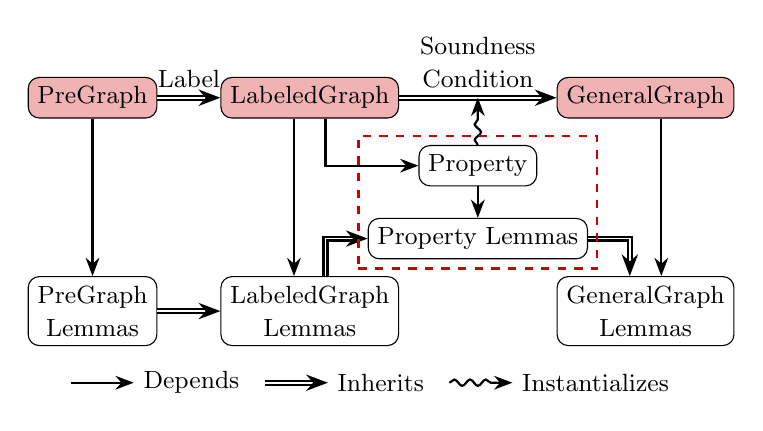
\begin{tikzpicture}
[->/.style={thick,arrows={-Stealth}},
-->/.style=	{thick,arrows={-Stealth}, decorate, decoration={snake, amplitude=.4mm,segment length=2mm,post length=2mm}},
   realG/.style={shape=rectangle, rounded corners=4pt, draw, fill=red!30},
   propG/.style={shape=rectangle, rounded corners=4pt, draw}]
\node[realG] (PG) at (0, 0) {\small PreGraph};
\node[realG] (LG) [right=0.8 of PG] {\small LabeledGraph};
\node[realG] (GG) [right=2 of LG] {\small GeneralGraph};
\draw [double, ->] (PG) -- (LG) node [pos=0.5, above] {\small Label} ;
\draw [double, ->] (LG) -- (GG) node (SC) [pos=0.5, above, align=center]
{\small Soundness \\ \small Condition};
\node[propG] (Prop) [below=0.6 of SC] {\small Property};
\node[propG] (PropL) [below=0.4 of Prop] {\small Property Lemmas};
\node[propG] (PGL) [below=2 of PG, align=center] {\small PreGraph \\\small Lemmas};
\node[propG] (LGL) [below=2 of LG, align=center] {\small LabeledGraph \\\small Lemmas};
\node[propG] (GGL) [below=2 of GG, align=center] {\small GeneralGraph \\\small Lemmas};
\draw [double, ->] (PGL) to (LGL);
\draw [->] (PG) to (PGL);
\draw [->] (Prop) to (PropL);
\draw [-->] (Prop) to (SC);
\coordinate [left=0.2 of LG.south] (LGs1);
\coordinate [left=0.2 of LGL.north] (LGLn1);
\draw [->] (LGs1) to (LGLn1);
\coordinate [right=0.2 of LG.south] (LGs2);
\coordinate [right=0.2 of LGL.north] (LGLn2);
\draw [->] (LGs2) |- (Prop);
\draw [double, ->] (LGLn2) |- (PropL);
\coordinate [right=0.2 of GG.south] (GGs);
\coordinate [left=0.2 of GGL.north] (GGLn1);
\coordinate [right=0.2 of GGL.north] (GGLn2);
\draw [double, ->] (PropL) -| (GGLn1);
\draw [->] (GGs) to (GGLn2);
\node [draw=red, thick, rectangle, dashed, fit=(Prop) (PropL)] {};
\node (legend1) [below right=0.2 and -0.3 of PGL] {\small Depends};
\coordinate[left=0.8 of legend1]  (l1);
\draw [->] (l1) to (legend1);
\node (legend2) [right=1 of legend1] {\small Inherits};
\coordinate[left=0.8 of legend2]  (l2);
\draw [double, ->] (l2) to (legend2);
\node (legend3) [right=1 of legend2] {\small Instantializes};
\coordinate[left=0.8 of legend3]  (l3);
\draw [-->] (l3) to (legend3);
\end{tikzpicture}
\end{adjustbox}
\captionof{figure}{Structure of the Mathematical Graph Library}\label{fig:graphs}
\end{minipage}
  ~
  \hspace{0em}
  \begin{minipage}[t]{0.5\textwidth}
  \begin{adjustbox}{scale=0.80}
\centering
\hspace{1.8em}
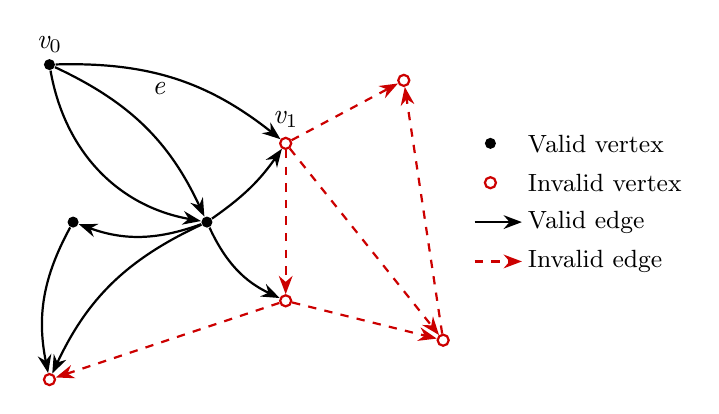
\begin{tikzpicture}
[vad/.style={circle, fill=black, inner sep=0pt, minimum size=4pt},
 inv/.style={circle, draw=red, thick, inner sep=0pt, minimum size=4pt},
 ->/.style={thick, arrows={-Stealth}}]
\node[vad] (n1) at (0, 0) {};
\node at (1, 1.3) {$\m{v}_1$}; \node[inv] (n2) at (1, 1) {};
\node[inv] (n3) at (1, -1) {}; \node at (-2,2.25) {$\m{v}_0$}; \node[vad] (n4) at (-2,2) {}; 
\node[inv] (n5) at (-2,-2) {};
\node[vad] (n6) at (-1.7,0) {};
\node[inv] (n7) at (2.5,1.8) {};
\node[inv] (n8) at (3,-1.5) {};
\draw[->] (n1) to [bend right=10] (n2);
\draw[->] (n1) to [bend right=20] (n3);
\draw[->,dashed,red] (n3) to (n5);
\draw[->,dashed,red] (n3) to (n8);
\draw[->,dashed,red] (n2) to (n3);
\draw[->,dashed,red] (n2) to (n7);
\draw[->,dashed,red] (n2) to (n8);
\draw[->,dashed,red] (n8) to (n7);
\draw[->] (n4) to [bend left=20] (n1);
\draw[->] (n1) to [bend right=20] (n5);
\draw[->] (n4) to [bend left=20] (n2);
\draw[->] (n1) to [bend left=20] (n6);
\draw[->] (n6) to [bend right=20] (n5);
\draw[->] (n4) to [bend right=35] (n1);
\node at (-0.6, 1.7) {$\m{e}$};
\node[vad] (n9) at (3.6, 1) {};
\node[inv] (n10) at (3.6, 0.5) {};
\draw[->] (3.4, 0) -- (4, 0);
\draw[->,dashed,red] (3.4, -0.5) -- (4, -0.5);
\node at (3.9, 1) [right=1.5pt] {\small Valid vertex};
\node at (3.9, 0.5) [right=1.5pt] {\small Invalid vertex};
\node at (3.9, 0) [right=1.5pt] {\small Valid edge};
\node at (3.9, -0.5) [right=1.5pt] {\small Invalid edge};

\end{tikzpicture}
\end{adjustbox}

\captionof{figure}{PreGraph with valid/invalid vertices/edges.}\label{fig:pregraph}
\end{minipage}
\vspace{1.5ex}

 
\subsection{Definitions of Graphs}\label{sec:mathinfra}

Our first challenge is that graph theory is usually based on
\emph{set theory} but our formalization in Coq is
based on \emph{type theory}. 
Instead of formalizing set theory in Coq and then building
graph theory atop it, we formalize graph theory
directly in Coq, as this lets us take advantage of Coq's built-in
support for type-related constructions.
To reconcile the dichotomy between
a very general library and highly specialized examples, we develop
our graphs gradually over three linked concepts:
PreGraph, LabeledGraph and GeneralGraph.
Figure~\ref{fig:graphs} shows the
architecture of the library.

\hide{The most basic kind of graph is PreGraph, out of which we build
LabeledGraph, and which in turn are used
to build GeneralGraphs. Each kind has some lemmas and also inherits the lemmas of the
previous kind.  The dashed box represents a ``plugin'' system for attaching arbitrary
properties to LabeledGraphs (\ref{subsec:graphplugins}). } 

\paragraph{PreGraph.}
A PreGraph is a hextuple $(\mathcal{V}, \mathcal{E}, \mathtt{V}, \mathtt{E}, \mathtt{src}, \mathtt{dst})$.  Arguments $\mathcal{V}$ and $\mathcal{E}$ are the underlying
carrier types of vertices and edges.  $\mathtt{V}$ and $\mathtt{E}$ are predicates over
$\mathcal{V}$ and $\mathcal{E}$ that specify the notion
of \emph{validity} in the graph.  Finally, $\mathtt{src}$ and $\mathtt{dst}$ map each edge to
its source and destination.


The benefits of introducing validity are twofold. The first is a
neat resolution of the incompatibility between type theory and set theory.
In set theory, one
element can belong to multiple sets, and
adding or removing vertices or edges is as easy as altering
the set directly to represent the result of the operation.
In type theory, however, a term can only belong
to one type, which makes it difficult\hide{if not impossible}
to analogously change the
type to represent the result. As is common practice, the
predicates $\mathtt{V}$ and $\mathtt{E}$ specify whether a vertex/edge is \emph{valid}
(in the graph) or \emph{invalid} (out). Adding or removing vertices/edges
is as simple as weakening or strengthening these two predicates.

The second benefit is the ability to represent incomplete graphs.
Consider starting from a graph~$\gamma$ and then removing a subgraph; the remaining
``doughnut'' structure is \textbf{not} necessarily a graph, since there may be dangling
edges pointing into the ``hole''.  Figure \ref{fig:pregraph} shows just such a situation,
where a connected graph (everything that is reachable from $\m{v}_0$) has had the connected
subgraph reachable from $\m{v}_1$ removed, thus leaving the edge $e$ dangling.
The last conjunct in the $\m{findS}$ relation from Figure~\ref{fig:find} is an example
of where a real verification needs to reason about just such a doughnut, in particular
to specify that the unreachable portion of a graph has not changed.


\hide{an incomplete graph,
where vertices $v_0$ and $v_1$
are the source and destination of a valid edge $e_0$. Both
vertices are in $\mathcal{V}$, but $v_0$ is valid
and $v_1$ is not, meaning $v_1$ is not in the
graph. Drawing $v_1$ in Figure \ref{fig:pregraph} only indicates
that $d(e_0) = v_1$.
Incomplete graphs of this sort are needed, \emph{e.g.}, by programs
that traverse selective portions of graphs and manipulate them under
certain criteria.
After the traversal, the graph $g$ can be partitioned into two parts: the subgraph
$g_1$, which is composed of vertices and edges processed by the algorithm,
and the residue $g_2$, which is the difference $g - g_1$. In
the specification of the program, it may be necessary to state that
$g_2$ is unchanged. However, $g_2$ is not guaranteed to be a ``well-formed''
graph in the conventional sense:
if $g$ is an undirected graph,
$g_2$ is just a collection of \note[disconnected?]{connected} components,
and if $g$ is a directed graph, then $g_2$ may contain dangling edges or
vertices. PreGraph is accommodating enough to permit reasoning
about~$g_2$ in either case.}

\begin{figure}
  \begin{minipage}{.52\textwidth}
  \begin{equation*}
  {\footnotesize
  \begin{array}{r@{}c@{}l}
    	\mathrm{path} \; &\defeq \;& (\m{v}_0, [e_0, e_1, \dots, e_k]) \\
      \mathtt{end}\big(\gamma, (\m{v}, [])\big)\;&\defeq\;& \m{v}\\
      \mathtt{end}\big(\gamma, (\m{v},[e_1,\dots,e_n])\big)\;&\defeq\;&
      \mathtt{dst}_{\gamma}(e_{n}) \\
      \mathtt{s\_evalid}(\gamma, e) \; &\defeq \;& \mathtt{E}_{\gamma}(e) /| \null \\
      &&\mathtt{V}_{\gamma}(\mathtt{src}_{\gamma}(e)) /| \null \\
      &&\mathtt{V}_{\gamma}(\mathtt{dst}_{\gamma}(e)) \\
      \mathtt{valid\_path}\big(\gamma, (\m{v},[])\big) \;&\defeq \;& \mathtt{V}_{\gamma}(\m{v})\\
      \mathtt{valid\_path}\big(\gamma, (\m{v},[e_1,e_2,\dots,e_n])\big) \; &\defeq \;& \m{v}=\mathtt{src}_{\gamma}(e_1) \wedge \null \\
      &&\mathtt{s\_evalid}(\gamma,e_1) \wedge \null \\
      &&\mathtt{dst}_{\gamma}(e_1)=\mathtt{src}_{\gamma}(e_2) \wedge \null \\
      &&\mathtt{s\_evalid}(\gamma, e_2) \wedge \dots /| \null \\
      &&\mathtt{dst}_{\gamma}(e_{n-1})=\mathtt{src}_{\gamma}(e_n)
  \end{array}}
  \end{equation*}
  \end{minipage}\begin{minipage}{.5\textwidth}
  \begin{equation*}
  {\footnotesize
  \begin{array}{r@{}c@{}l}
      \gamma_1 \cong \gamma_2 \; &\defeq\;&
        \forall e.~\mathtt{E}_{\gamma_1}(e) <=> \mathtt{E}_{\gamma_2}(e) /| \null \\
        &&\forall \m{v}.~\mathtt{V}_{\gamma_1}(\m{v}) <=> \mathtt{V}_{\gamma_1}(\m{v}) /| \null \\
        &&\forall e.~\mathtt{E}_{\gamma_1}(e) ==> \mathtt{src}_{\gamma_1}(e) = \mathtt{src}_{\gamma_2}(e) /| \null \\
        &&\hspace{5.9em} \mathtt{dst}_{\gamma_1}(e) = \mathtt{dst}_{\gamma_2}(e) \\
      \gamma |= s \overset{\m{p}}{\leadsto} t \;&\defeq\;&
        \mathtt{valid\_path}(\gamma, p)\wedge \null \\
        &&\mathtt{fst}(p)=s \wedge \mathtt{end}(\gamma,p)=t \\
      \gamma \smallsetminus S \; &\defeq \;&
          \Big(\mathcal{V}_{\gamma},\mathcal{E}_{\gamma}, \mathtt{src}_{\gamma}, \mathtt{dst}_{\gamma}, \\
          &&\qquad \lambda x.~ \gamma_{\mathtt{V}}(x) /| \lnot S_{\mathtt{V}}(x), \\
          &&\qquad \lambda x.~ \gamma_{\mathtt{E}}(x) /| \lnot S_{\mathtt{E}}(x)\;\Big)
  \end{array}}
  \end{equation*}
  \end{minipage}
\vspace{-.7em}
\caption{Some PreGraph definitions}
\label{fig:pregraphdefs}
\vspace{-1em}
\end{figure}

%
 
We define many fundamental graph concepts on PreGraphs,
including structures like \emph{path}$^{*}$, predicates
such as \emph{is\_cyclic} and \emph{reachable}$^{*}$,
operations such as \emph{add\_vertex}
and \emph{remove\_edge}, and relations between PreGraphs such
as \emph{structurally\_identical}$^{*}$ and \emph{subgraph}.
Definitions of the concepts marked with asterisks are
shown in Figure \ref{fig:pregraphdefs} to give a flavor
of the subtleties involved in getting definitions that
really work.
These general concepts, together with around 500 derived lemmas,
provide a
solid foundation for more specific theorems needed in concrete
verifications.

\hide{
In {\color{magenta}Figure \ref{fig:pregraph}}, valid vertices satisfy
$V$ and invalid vertices are just of type $VT$ but do not satisfy
$V$. Importantly, both kinds of vertices are legally part of the
PreGraph. Finally, $s$ and $d$ are functions that map an edge to its
source and destination respectively; {\color{orange}this means that
PreGraphs model directed graphs.}  With an eye to flexibility, we make
no further requirements of a legal PreGraph, not even a specific
notion of how the four sets are related.  Indeed, the PreGraph in
Figure \ref{fig:pregraph} contains invalid vertices and edges in an
arbitrary configuration.

Many graph concepts such as \emph{path}, \emph{reachability}, and \emph{subgraph} are
defined on PreGraphs. In \S\ref{fig:find} we saw \emph{reachable}, written
{\color{orange}
$\m{a} \mathrel{{\stackrel{\gamma~}{\leadsto^{1}}}} \m{b}$. It means that a and b are in $V(\gamma)$ and that there exists an edge (in $E(\gamma)$)
that goes from a to b.}
The reflexive, transitive closure on \emph{reachable} is written
$\m{a} \accentset{\gamma}{\leadsto}^{\star} \m{b}$, and
$\neg (\m{a} \accentset{\gamma}{\leadsto}^{\star} \m{b})$
is written
$\m{a} \accentset{\gamma}{\not\leadsto}^{\star} \m{b}$
$\m{a} \mathrel{{\stackrel{\gamma~}{\not\leadsto^{\star}}}} \m{b}$.

PreGraph's ability to reason about missing vertices and edges is convenient when
verifying real programs. Suppose some $\gamma$ satisfied some stronger notion of
``well-formed'', in the sense that valid vertices have only valid edges and
vice versa. Could we then subtract some vertices and edges from it and reason about the
resulting structure? This is precisely what we needed to do in \ref{fig:find}, where
we argued for a condition of congruence on
$\gamma \smallsetminus (v \in \gamma \mid \m{x}
\mathrel{{\stackrel{\gamma~}{\leadsto^{\star}}}} \m{v})$.
A strong notion of well-formedness may have stopped us short at this point,
declaring the structure ill-formed because of the dangling edges
pointing to recently-removed vertices.
A PreGraph is more accommodating, since
it produces a fresh PreGraph after this selective subtraction
and then allows us to go ahead and reason about congruence as we need to.
}

\hide{
For example, consider the difference of two graphs, $\gamma_1
- \gamma_2$.  Even if both of these graphs are ``well-formed'' to begin with, in the
sense that valid vertices have only valid edges and vice versa, their difference
may not be since there may be dangling edges pointing to the
now-removed vertices of $\gamma_2$.} 

\hide
{In \S\ref{sec:spacegraph} we will tie a mathematical graph $\gamma$ to
a spatial graph predicate
$\p{graph}(x, \gamma)$.   As we will see, a $\p{graph}$ ``owns'' only the
spatial portion of $\gamma$ that is reachable
from $x$ even though $\gamma$ may have other valid vertices.
} 




\vspace{-0.75ex}

\paragraph{LabeledGraph.}
A LabeledGraph is septuple $(\mathrm{PreGraph},\ma{L_{V}},\ma{L_{E}},\ma{L_{G}}, \mathtt{vl},\mathtt{el},\mathtt{gl})$ that augments a PreGraph with \emph{labels} on
vertices, edges, and/or the graph as a whole. $\ma{L_{V}}$, $\ma{L_{E}}$, and $\ma{L_{G}}$
are the associated carrier types, and $\mathtt{vl}$, $\mathtt{el}$, and $\mathtt{gl}$
are the labeling functions themselves.
Many classic graph problems, from union-find (node ranks)
to Dijkstra (edge weights), require such labels.
The need for a label on the graph as a whole
is not as obvious; in \S\ref{sec:certigc} we use one in the garbage collector
to keep track of the number of generations and their boundaries.
Since every LabeledGraph is built on a PreGraph, it inherits all of the 
PreGraph's lemmas via
Coq's \emph{type coercion} mechanism while also opening the doors to 
additional lemmas involving its own labels.



\hide{\paragraph{LabeledGraph.}
A LabeledGraph is a PreGraph with the addition of \emph{labels} on
vertices, edges, and/or the graph as a whole. The need for such labels
is fairly clear; the bare structure of a graph can only
contain so much information, and many classic graph problems
such as graph coloring, shortest path, and network flow rely on
additional information in the form of labels. In our architecture, a
LabeledGraph inherits any lemmas proved about its associated PreGraph.
In addition, we can define additional lemmas that use labels,
\emph{e.g.} the union-find graph has an integer label denoting \emph{rank}.
We could prove a lemma that running \li{find} does not alter
any vertex's rank.
\hide{add string labels to edges and reason about a trie.}}




\vspace{-0.75ex}
\paragraph{GeneralGraph.}
PreGraphs and LabeledGraphs let us state
and prove many useful lemmas that follow essentially by the nature
of our graph constructions. However, when proving the correctness of graph
algorithms, we often need more specificity in our mathematical graphs
so that we may model the real program's behaviors closely.
For example, the \p{uf\_graph} used in \li{find}
restricts each vertex to having exactly one out-edge.
On the other hand, these restrictions vary greatly by algorithm, so we do not
want to bake them into our core definitions.
We achieve this flexibility using GeneralGraphs, which augment
LabeledGraphs by adding arbitrarily complex ``soundness conditions'', indicated in
Figure~\ref{fig:graphs} with a dashed border.
Further, the type coercion we described earlier continues to apply,
meaning that a GeneralGraph can seamlessly behave like its internal
LabeledGraph or a PreGraph, thereby inheriting their lemmas.
This combination of specificity and generality
makes GeneralGraphs versatile. Moreover, we can
compose complicated soundness conditions from reusable pieces,
further enabling code sharing between algorithms.







\subsection{Composing Soundness Plugins}
\label{subsec:graphplugins}
\begin{figure}
{\footnotesize
\begin{align*}
  \mathrm{MathGraph}(\gamma)\,& \defeq \,\left\{
  \begin{aligned}
    \mathtt{null}:&\; V\\
    \mathtt{valid\_graph}:&\;
    \forall e\,.\,\mathtt{evalid}(\gamma, e) \Rightarrow
      \mathtt{vvalid}\big(\gamma, \mathtt{src}(\gamma, e)\big)\wedge
      \big(\m{e} = \mathtt{null} \vee \mathtt{vvalid}(\gamma, \m{e})\big)\\
    \mathtt{valid\_not\_null}:&\; \forall \m{v}\,.\,\mathtt{vvalid}(\gamma, \m{v})
    \Rightarrow \m{v} \neq \mathtt{null}
  \end{aligned} \right\}\\
  \mathrm{LstGraph}(\gamma)\,&\defeq\, \left\{
  \begin{aligned}
    \mathtt{out}:&\; V \rightarrow E\\
    \mathtt{only\_one\_edge}:&\;
    \forall \m{v},\,e\,.\,\mathtt{vvalid}(\gamma, \m{v}) \Rightarrow
    \big(\mathtt{src}(\gamma, e) =\m{v} \wedge
    \mathtt{evalid}(\gamma, e)\big) \Leftrightarrow e = \mathtt{out}(\m{v})\\    
  \mathtt{acyclic\_path}:&\; \forall \m{v},\,p\,.\,
  \gamma |= \m{v} \overset{p}{\leadsto} \m{v} \Rightarrow p = (\m{v},[]) \\
  \end{aligned} \right\}\\
  \mathrm{FiniteGraph}(\gamma)\,&\defeq\, \left\{
  \begin{aligned}
      \mathtt{finite\_v}:&\;\exists\, S_\m{v},\, M_\m{v}.~\;\lvert S_\m{v}\rvert
      \leq M_\m{v} \wedge
      \forall \m{v}\,.\, \mathtt{vvalid}(\gamma,\m{v})\Rightarrow \m{v}\,\in\,S_\m{v}\\
      \mathtt{finite\_e}:&\;\exists\, S_e,\, M_e.~\;\lvert S_e\rvert
      \leq M_e \wedge
      \forall e\,.\, \mathtt{evalid}(\gamma,e)\Rightarrow e\,\in\,S_e\\
  \end{aligned}  \right\}\\
\end{align*}}
\vspace*{-3em}
\caption{Some GeneralGraph definitions}
\label{fig:gengraphdefs}
\vspace{-1.5em}

\end{figure} 
 
\hide{Our entire library of formal
graph theory is developed around the
three graph structures above. The theorems about the first two
are universal, while some theorems about GeneralGraph
are developed on demand because soundness conditions vary by
algorithm.}
Soundness conditions are often specific to each algorithm, but they feature some recurring themes.
We take advantage of this pattern by developing \emph{soundness plugins}, \emph{i.e.} definitions of soundness
conditions along with related lemmas.  By combining these plugins
we can describe the soundness condition we need for a particular
algorithm.  When proving lemmas about the resulting combination,
we can use known facts about the separate plugins, in addition to
lemmas that emerge due to the various combinations.  This complexity
is managed smoothly by Coq's typeclass system, increasing the
compositionality of the system.
Consider the following oft-used graph properties:

\begin{itemize}
\vspace{-1ex}
\item \p{BiGraph}: there are exactly two outgoing edges per vertex
\item $\p{LstGraph}^{*}$: the graph is structured like a list, meaning that every 
vertex has one outgoing edge, and there no loops except trivial self-loops 
of length $0$, signifying the end of the ``list"
\item $\p{MathGraph}^{*}$: every valid edge has a valid source vertex,
and its destination vertex is either valid or is a 
special invalid vertex called \p{null}
\item $\p{FiniteGraph}^{*}$: the sets of valid vertices and edges are both finite
\hide{More subtly, consider that many real data structures use special null values to
represent unused nodes.  The  property introduces this concept---
\emph{i.e.} some special invalid nodes are allowed to appear as
destinations for valid edges.} 



\end{itemize}
Definitions of the concepts marked with asterisks are
shown in Figure~\ref{fig:gengraphdefs} for illustration.
\hide{As a first step, we can prove many general, reusable lemmas
about these properties. However, these properties are still
too general to model a real program. The next step is to compose
these plugins to arrive at a more specific set of restrictions
that more closely models our particular graph.}
We can compose
\p{LstGraph}, \p{MathGraph}, and \p{FiniteGraph}
together into a new plugin called \p{LiMaFin}, which, incidentally, is
the soundness condition of mathematical \p{uf\_graph}
we used to verify \li{find} in
Figure~\ref{fig:find}.  In our verification of \li{mark} in
Figure~\ref{fig:markgraph}, we use a similar soundness condition
\p{BiMaFin}, which uses \p{BiGraph} instead of \p{LstGraph}.
The commonalities and differences between \p{LiMaFin}
and \p{BiMaFin} are readily apparent from their construction, 
and can be exploited for proof reuse.


\iffalse
\marginpar{\tiny \color{blue} Maybe move this somewhere.}
{\color{magenta}Coq also handles our notion of inherited
lemmas seamlessly: in our verfication of Find, we
work directly with a \p{LiMaFin} GeneralGraph, but, as
we saw, we still use properties such as reachability
and operations such as selective subtraction, which are defined on the
embedded PreGraph, not the GeneralGraph.
Coq handles the appropriate coercions with
remarkable elegance.}
\fi

\iffalse
\subsection{Reasoning about relations between graphs} 

\marginpar{\color{blue} \tiny Needs revised examples based on new Orientation.}

{\color{magenta} In Figure~\ref{fig:markgraph} we defined the relation
$\m{mark}(\gamma, \tx x, \gamma')$
for the graph marking algorithm.  Similarly, we define $\m{span}$ for the
spanning tree program
and $\m{copy}$ for the graph copy program.
These relations all capture how the graph has changed from before to after the program
execution.  By specifying $\m{copy}$ relationally
rather than functionally we avoid explicitly modeling how the memory
allocator works, a major advantage.

As previously mentioned, we reuse $\m{mark}$ and its
related lemmas to prove facts about spanning tree and graph copy
because the latter two programs mark nodes as they work.
Accordingly, we can reuse facts such as the following:
\[
\begin{array}{@{}l@{}}
\text{if } \gamma(x)=(0, v_1, \dots,v_n), \m{mark1}(\gamma, x, \gamma_1),
\text{ and } \forall i, \m{mark}(\gamma_i,v_i,\gamma_{i+1}) \text{ then } \m{mark}(\gamma,x,\gamma_{n+1}).
\end{array}
\]
}
\fi
 
\section{Defining and reasoning about spatial graphs}
\label{sec:spacegraph}


To prove the functional correctness of graph-manipulating algorithms implemented in a real language, we need to 
(1) connect the heap representation of graphs to the memory model of the 
programming language, and (2) connect the memory model to the mathematical 
properties of abstract graphs from \S\ref{sec:mathgraph}.
The first of these challenges turns out to be surprisingly subtle: 
the standard tactic of leveraging the \infrulestyle{Frame} rule 
works well for tree-manipulating programs, but fails for graph-manipulating programs.
We review the standard treatment for trees~(\S\ref{sec:seplogtrees}), 
point out the issue with graphs~(\S\ref{sec:fixpointfail}),
and propose a fix for this~(\S\ref{sec:goodgraph}).  
The main challenge thereafter is to engineer a framework that is generic 
and modular enough to be useful in a variety of 
settings~(\S\ref{sec:ramifylib}).

\begin{figure}
{\footnotesize
\[
\begin{array}{lcl}
\sigma |= P * Q & \defeq & \exists \sigma_1, \sigma_2.~ (\sigma_1 \oplus \sigma_2 = \sigma) /| (\sigma_1 |= P) /| (\sigma_2 |= Q)\\
\sigma |= P --* Q & \defeq & \forall \sigma_1, \sigma_2.~ (\sigma_1 \oplus \sigma = \sigma_2) /| (\sigma_1 |= P) => (\sigma_2 |= Q) \\
\sigma |= P ** Q & \defeq & \exists \sigma_1, \sigma_2, \sigma_3.~ (\sigma_1 \oplus \sigma_2 \oplus \sigma_3 = \sigma) /| (\sigma_1 \oplus \sigma_2 |= P) /| (\sigma_2 \oplus \sigma_3 |= Q)
\end{array}
\]
}
\vspace{-1em}
\caption{Separation logic connectives; $\oplus$ is the join operation on states, \emph{e.g.} a disjoint union on heaps}
\label{fig:seplogsem}
\vspace*{-1em}
\end{figure}  
\subsection{Separation Logic in Tree-Manipulating Programs}
\label{sec:seplogtrees}

Figure~\ref{fig:seplogsem} shows the standard semantic models for the separation logic connectives using a join relation $\oplus$ on an underlying separation algebra~\cite{dockins09}. In recent works \citep{o2001local, o2012primer}
that employ separation logic to give
precise specifications of tree copy programs, the spatial
representation of a binary tree is defined as a recursive predicate
with an additional parameter: the mathematical tree $\tau$.
\begin{equation}\label{def:tree}
\begin{split}
    \mathsf{tree}(x, \tau)\;\defeq\;
    &\Big(x=0 \wedge \mathsf{isatom}(\tau) \wedge \mathsf{emp}\Big)
    \vee \null \\ &\Big(\exists\,l,r,\tau_1,\tau_2.\; \tau=\langle \tau_1,
    \tau_2 \rangle \wedge (x \mapsto l,r) \scon
    \mathsf{tree}(l, \tau_1) \scon \mathsf{tree}(r, \tau_2)\Big)
    \end{split}
\end{equation}

The mathematical tree $\tau$ encodes the
shape of a binary tree. It is either an $\mathsf{atom}$ or a pair of
tree encodings. For example,
$\langle \mathsf{atom}, \langle \langle \mathsf{atom}, \mathsf{atom} \rangle, \mathsf{atom} \rangle \rangle$
is a valid encoding. A $\mathsf{tree}(x, \tau)$ is either an
$\mathsf{emp}$ or $(x \mapsto
l,r) \scon \mathsf{tree}(l, \tau_1) \scon \mathsf{tree}(r, \tau_2)$
where $\tau_1$ and $\tau_2$ are the left and right subtrees of $\tau$.
If $\tau_1$ is $\mathsf{atom}$ then $l$ must be null pointer and
$\mathsf{tree}(l, \tau_1)$ must be~$\mathsf{emp}$.
Otherwise $\mathsf{tree}(l, \tau_1)$ can be expanded recursively as above.
The left part of Figure~\ref{fig:bin_tree_graph} shows a binary tree, 
and it should be straightforward to see that the data layout matches~$\tau$ 
(the shape of the tree) exactly. In the verification of a tree
copy program, the precondition is $\mathsf{tree}(x, \tau)$ and the
postcondition is
$\mathsf{tree}(x, \tau) \scon \mathsf{tree}(y, \tau)$. 
Having the same $\tau$ in the pre- and postconditions
of the specification indicates that the program creates an exact clone
of the original tree, not an arbitrarily-shaped tree.

This is an ideal use-case for the separation logic
because the root, the left subtree, 
and the right subtree are disjoint by construction. By applying
the \textsc{Frame} rule, one can safely reason about a particular 
$\scon$-separated branch of the tree and later compose the 
conclusion back into the rest of the tree
without worrying about the effect on the rest of the tree. 
In the figure we show that manipulating the subtree under 
root~$\m{v}$ does not affect the rest of the tree.

Graphs are more complicated.
Consider the right part of Figure~\ref{fig:bin_tree_graph},
which shows a bigraph. 
Defining a recursive predicate in the style of \eqref{def:tree},
\emph{i.e.} using the separating conjunction~$\scon$, is a bad idea: 
a node can be shared arbitrarily, and so finding a suitable 
\infrulestyle{frame} is difficult. 
In the figure we show that manipulating the subgraph reachable 
from~$\m{w}$ causes an unexpected node to be affected.

\begin{figure}[htbp]
\centering
\begin{minipage}{.5\textwidth}
  \centering
  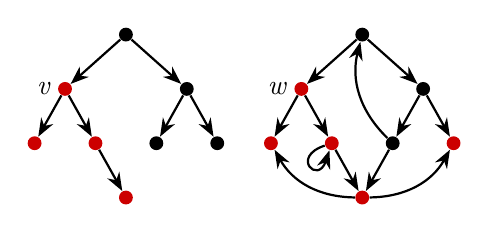
\begin{tikzpicture}[
  gnode/.style={circle, inner sep=0pt, minimum size=5pt, fill=black},
  gnodecol/.style={circle, inner sep=0pt, minimum size=5pt, fill=red},
  ->/.style={-Stealth, thick}, node distance=0.5cm]
  \node[gnode] (n0) {};
  \node[gnodecol] (n1) [below = of n0, xshift=-22pt] {};
  \node [left = of n1, xshift = 16pt] {$\m{v}$};
  \node[gnode] (n2) [below = of n0, xshift=22pt] {};
  \node[gnodecol] (n3) [below = of n1, xshift=-11pt] {};
  \node[gnodecol] (n4) [below = of n1, xshift=11pt] {};
  \node[gnode] (n5) [below = of n2, xshift=-11pt] {};
  \node[gnode] (n6) [below = of n2, xshift=11pt] {};
  \node[gnodecol] (n7) [below = of n4, xshift=11pt] {};
  \draw[->] (n0) to (n1);
  \draw[->] (n0) to (n2);
  \draw[->] (n1) to (n3);
  \draw[->] (n1) to (n4);
  \draw[->] (n2) to (n5);
  \draw[->] (n2) to (n6);
  \draw[->] (n4) to (n7);
  \node[gnode] (m0) [right = 80pt of n0]{};
  \node[gnodecol] (m1) [below = of m0, xshift=-22pt] {};
  \node [left = of m1, xshift = 16pt] {$\m{w}$};
  \node[gnode] (m2) [below = of m0, xshift=22pt] {};
  \node[gnodecol] (m3) [below = of m1, xshift=-11pt] {};
  \node[gnodecol] (m4) [below = of m1, xshift=11pt] {};
  \node[gnode] (m5) [below = of m2, xshift=-11pt] {};
  \node[gnodecol] (m6) [below = of m2, xshift=11pt] {};
  \node[gnodecol] (m7) [below = of m4, xshift=11pt] {};
  \draw[->] (m0) to (m1);
  \draw[->] (m0) to (m2);
  \draw[->] (m1) to (m3);
  \draw[->] (m1) to (m4);
  \draw[->] (m2) to (m5);
  \draw[->] (m2) to (m6);
  \draw[->] (m4) to (m7);
  \draw[->] (m5) to (m7);
  \draw[->] (m5) to [bend left] (m0);
  \draw[->] (m4) .. controls ([xshift=-15pt, yshift=-5pt] m4) and ([xshift=-5pt, yshift=-15pt] m4) .. (m4);
  \draw[->] (m7) to [bend right] (m6);
  \draw[->] (m7) to [bend left] (m3);
\end{tikzpicture}
   \captionof{figure}{A Binary Tree and a Binary Graph}
  \label{fig:bin_tree_graph}
\end{minipage}\begin{minipage}{.5\textwidth}
  \centering
  \vspace*{0.5em}
  \begin{tabular}[b]{c|c}
\textrm{address} & \textrm{value} \\
\hline
102 & 0 \\
101 & 100 \\
100 & 42 \\
\end{tabular}
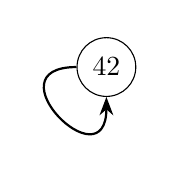
\begin{tikzpicture}
[->/.style={thick,arrows={-Stealth}},
   propG/.style={shape=circle, draw}]
   \path[use as bounding box] (-1, -1) rectangle (0.5, 0.5);
   \node[propG] (P) at (0, 0) {42};
   \draw[->] (P.west) .. controls (-1.5, 0) and (0, -1.5) .. (P.south);
\end{tikzpicture}
   \vspace*{1em}
  \captionof{figure}{A One-Cell Graph and its Heap Layout}
  \label{fig:single:cell}
\end{minipage}
\end{figure}

\subsection{Recursive Definitions Yield Poor \p{graph} Predicates}\label{sec:fixpointfail}

\newcommand{\graphkt}{\p{graph}_T}
\newcommand{\grapham}{\p{graph}_A}


Recursive predicates are ubiquitous in separation logic---so
much so that when one writes the definition of a predicate as
\mbox{$P$ ``$\defeq$'' $\ldots P \! \ldots$}, no one raises an eyebrow despite the
dangers of circularity in mathematics. Indeed, the vast majority of the time there
is no danger thanks to the magic of the Knaster-Tarski fixpoint
$\mu_{\mathsf{T}}$ \cite{tarski:fixpoint}.  Formally, one does not define $P$ directly,
but rather defines a functional
\mbox{$F_P \defeq \lambda P.~ \ldots P \! \ldots$} and then defines $P$ itself as
\mbox{$P \defeq \mu_{\mathsf{T}} \, F_P$}.
Assuming, as one typically does without comment,
that $F_P$ is \emph{covariant}, i.e. $(P |- Q)
\Rightarrow (F \, P |- F \, Q)$, one then enjoys the fixpoint
equation $P \Leftrightarrow \ldots P \ldots$, formally justifying
the typically-written pseudodefinition (``$\defeq$'').



Suppose we define a graph predicate $\graphkt$ along the lines of the fold/unfold definition in Figure~\ref{fig:markgraph}.  Such a definition would use the overlapping conjunction $P ** Q$ (\emph{c.f.} Figure~\ref{fig:seplogsem}) as follows: \vspace{-1ex}
\[
\begin{array}{@{}l@{}l@{}}
\graphkt(x, \gamma) \; \defeq \; &\Big(x = 0 /| \p{emp}\Big) |/ \\
&\quad \Big(\exists m,l,r.~ \gamma(x)=(m,l,r) /|
\big(x |-> m,l,r ** \graphkt(l, \gamma) ** \graphkt(r, \gamma)\big)\Big)
\end{array}
\vspace{-1ex}
\]
Although we can apply Knaster-Tarski (because the functional needed to
define $\graphkt$ is covariant), the result is hard to use.
Consider the memory $m$ for a toy machine, where $m |= 100 |-> 42,100,0$.
It seems clear, however, that this
memory also represents a one-cell cyclic graph as illustrated in
Figure~\ref{fig:single:cell}, \emph{i.e.} we want
$m |= \graphkt(100,\hat{\gamma})$, where 
$\hat{\gamma}(100) = (42,100,0)$.  This is equivalent to wanting to be able to 
prove $100~|->~42,100,0~|-~\graphkt(100,\hat{\gamma})$.  Unfortunately, as 
illustrated in Figure~\ref{fig:badcycle}, this is rather difficult to do since 
applying the natural proof techniques actually strengthens the goal.
Part of the 
problem is that the recursive structure interacts very badly with $**$: if the 
recursion involved~$*$~then it \textbf{would} be provable, by induction on the 
finite memory (each ``recursive call'' would be on a strictly smaller subheap).  
This is why Knaster-Tarski works so well with list, tree, and DAG predicates in 
separation logic.  We do not know if this entailment is provable, but the 
difficulties encountered in proving what ``should be'' straightforward suggest 
that Knaster-Tarski should be treated with caution when defining spatial 
predicates for graphs.

\begin{figure}[htbp]
\[
\infrule{}
{\infrule{}
  {100 |-> 42,100,0 ~ |- ~ 100 |-> 42,100,0 ** \graphkt(100,\hat{\gamma})}
  {100 |-> 42,100,0 ~ |- ~ \hat{\gamma}(100) = (42,100,0) ~ /| ~ 100 |-> 42,100,0 ** \graphkt(100,\hat{\gamma}) ** \graphkt(0,\hat{\gamma})}
  {\ddagger}
}
{100 |-> 42,100,0 ~ |- ~ \graphkt(100,\hat{\gamma})}
{\dagger}
\]
\begin{tabular}{@{}l@{$~~$}l|l@{$~~$}l}
$\dagger$ & Unfold $\graphkt$, dismiss first disjunct (contradiction), $~~$ & $~~$ $\ddagger$ &simplify using $P * \p{emp} -|- P$ \\
& introduce existentials (which must be 42,100,0) & & and remove pure conjunct
\end{tabular}
\caption{An attempt to prove a ``simple'' entailment}
\label{fig:badcycle}
\end{figure}


The other direction, \mbox{$\graphkt(100,\hat{\gamma}) |- 100 |-> 42,100,0$},
\textbf{is} true but is not easy to prove, relying on the constructions in \S\ref{sec:goodgraph} and the fact that $\mu_{\mathsf{T}}$ constructs the least fixpoint.  In contrast, $\graphkt(100,\hat{\gamma}) |- 100 |-> 42,100,0 * \top$ is easy. 

\hide{
\cite{appel:fixpoint} defined an alternative fixpoint using a notation of \emph{contractiveness}.  Unfortunately, this alternative fixpoint also
fails to define a sensible graph predicate; see Appendix~\ref{apx:appelfixpiont}.

\subsection{Problem with Appel and McAllester's fixpoint}
\label{apx:appelfixpiont} }

Appel and McAllester proposed another fixpoint $\mu_{\mathsf{A}}$
that is sometimes used to define recursive predicates in separation
logic \cite{appel:fixpoint}.  This time the functional $F_P$ needs to be
\emph{contractive}, which to a first order of approximation means that
all recursion needs to be guarded by~$\rhd$~, the ``approximation
modality'' \cite{appel:vmm}, \emph{i.e.} our graph predicate would
look like
\begin{align*}
\grapham(x, \gamma) ~ \defeq ~~ &(x = 0 /| \p{emp}) |/ \exists m,l,r.~ \gamma(x)=(m,l,r) /| \null \\
 & x |-> m,l,r ** \rhd \grapham(l, \gamma) ** \rhd \grapham(r, \gamma)
\end{align*}
This functional is contractive, and so the fixpoint is well-defined.  
Nevertheless, this definition has a subtle flaw: the resulting graph
predicate is \textbf{not} ``precise'' in the separation logic sense:
\[
\m{precise}(P) ~~ \defeq ~~ (\sigma_1 |= P) ~ => ~ (\sigma_2 |= P) ~ => ~ (\sigma_1 \oplus \sigma_1' \! = \! \sigma) ~ => ~ (\sigma_2 \oplus \sigma_2' \! = \! \sigma) ~ => ~ \sigma_1 \! = \! \sigma_2
\]
The flaw stems from the fact that $\rhd P$ is not precise for any $P$ 
(at time zero, $\rhd P$ is just $\top$), 
so $\grapham$ is not precise either.  The approximation modality's 
universal imprecision has never been noticed before in the literature.
Accordingly, $\grapham$ is also rather difficult to use.


\hide{
\section{Difficulty using $\graphkt$}
\label{apx:problemrecgraph}


See Figure \ref{fig:badcycle} for an attempt to prove the entailment $100 |-> 42,100,0 ~ |- ~ \graphkt(100,\hat{\gamma})$.  Part of the problem is that the recursive structure interacts very badly with $**$: if the recursion involved~$*$~then it \textbf{would} be provable, by induction on the finite memory (each ``recursive call'' would be on a strictly smaller subheap).  This is why Knaster-Tarski works so well with list, tree, and DAG predicates in separation logic.
}












\subsection{Defining a Good \p{graph} Predicate}\label{sec:goodgraph}

Rather than trying to define \p{graph} as a recursive fixpoint,
we will instead give it a flat structure.  Graphs in separation
logic have been defined in similar ways before, \emph{e.g.}~\citet{ilya-graphs};
our innovation is that we prove---with the amount of precision
required to convince Coq---that we can still enjoy fold/unfold
with our flat definition.  Our path starts with the iterated
separating conjunction or ``big star'', which is first defined over
lists and then extended to sets as follows:

\vspace{-1em}
\[
\begin{array}{@{}l@{}}
\!\!\!\!\!\!\!\underset{\{l_1,\dots,l_n\}}{\bigstar P}\!\!\!\!\!\!\! ~~ \defeq ~~ P(l_1) *
  P(l_2) * \dots * P(l_n) \quad \vline \quad
\underset{S}{\bigstar} P ~~ \defeq ~~ \exists L.~ (\p{NoDup}\ L) /| (\forall x.~ x\ \p{in}\ L <=> x \in S) /| \underset{L}{\bigstar}P
\end{array}
\]

We are now ready to define a good \p{graph} predicate:
  \quad $\p{graph}(x, \gamma) \; \defeq \; \!\!\!\!\!\!\!\!\!\!\underset{\m{v} \in \mathit{reach}(\gamma, x)}{\bigstar}\!\!\!\!\!\!\m{v}\mapsto\gamma(\m{v})$.
\iffalse
\begin{equation*}
  \underset{\{l_1, l_2,\dots,l_n\}}{\bigstar}P ~~ \defeq ~~ P(l_1) *
  P(l_2) * \dots * P(l_n).
\end{equation*}
Formally $\bigstar$ is defined over a list rather than a set and is parameterized by a predicate $P$.  It is natural to extend $\bigstar$ to a set $S$ with an existentially-quantified duplicate-free list~$L$:
\[
\underset{S}{\bigstar} P ~~ \defeq ~~ \exists L.~ (\p{NoDup}\ L) /| (\forall x.~ x\ \p{in}\ L <=> x \in S) /| \underset{L}{\bigstar}P
\]
We use the same $\bigstar$ notation since the concepts are similar, but the existential adds a little pain since we need to prove that all choices of $L$ yield equivalent predicates.

We are now ready to give a good \p{graph} predicate:
\fi


\hide{ \vspace{-1.5ex}
\begin{equation}\label{eqn:iter_def}
  \p{graph}(x, \gamma) ~~ \defeq ~~ \underset{v \in \mathit{reach}(\gamma, x)}{\bigstar} v\mapsto\gamma(v)
\vspace{-1.5ex}
\end{equation}
$\gamma$ is a GeneralGraph and ``$x |-> \gamma(x)$'' is a predicate that says how a single node fits in memory. In Figure~\ref{fig:markgraph} it was:
\[
\exists m,l,r.~\gamma(x) = (m,l,r) /| x |-> m,-,l,r /| x\ \p{mod}\ 16 = 0
\]}
The graph $\gamma$ here need not be a bigraph, but \emph{e.g.} can have many edges.

Our definition of \p{graph} is flat in the sense that there is no obvious way to follow the link structure recursively.  Happily, we can recover a general recursive fold/unfold (if $x |-> \gamma(x)$ and the GeneralGraph has the necessary properties in its soundness condition):
\vspace{-1ex}
\begin{equation}
\label{eqn:unfold_graph}
\hspace{-1em}\begin{array}{@{}lc@{\hspace{1pt}}c@{\hspace{1pt}}l@{}}
\p{graph}(x,\gamma)  <=>  x |-> \gamma(x) ** \big(\!\!\!\!\!\!\!\!\!\!\!\!\!\underset{n \in \p{neighbors}(\gamma,x)}{\bigocon}\!\!\!\!\!\!\!\!\!\!\!\! \p{graph}(\gamma,n) \big)
\quad \text{~~~ where ~~ }\underset{l_1,\dots,l_n}{\raisebox{-0.3ex}{\resizebox{0.75em}{!}{\hspace{0.05em}$\scon$}}\hspace{-2.18ex} \bigcup} \! \! P  \defeq  P(l_1) ** \ldots ** P(l_n) \end{array}
\vspace{-1ex}
\end{equation}

The proof of the $<=$ direction requires care. The difficulty is that if two nodes $x |-> \gamma(x)$ and $x' |-> \gamma(x')$ are \emph{skewed}, \emph{i.e.} ``partially overlapping'' with some---but not all---of $x$'s memory cells shared with $x'$, then the $\bigstar$ on the left hand side cannot separate them.  To avoid skewing we require that $x |-> \gamma(x)$ be \emph{alignable}. A predicate $P$ is alignable when
\[
\forall x,y.~ \Big(P(x) ** P(y) |- \big(P(x) /| x = y\big) |/ \big(P(x) * P(y)\big)\Big)
\]
That is, they overlap either completely or not at all. In a Java-like memory model this property is automatic because pointers in such a model always point to the root/beginning of an object.  In contrast, in a C-like memory model such as in VST/CompCert, this property is not automatic because pointers can point anywhere.  In such a model, alignment is most easily enforced by storing graph nodes at addresses that are multiples of an appropriate size (\emph{e.g} this size is $16$ in Figure~\ref{fig:markgraph}).

Some of our VST proofs, \emph{e.g.} for \li{find}, do not use fold/unfold, instead preferring to use the lemmas in~\S\ref{sec:ramifylib} directly.  Others, \emph{e.g.} \li{mark}, do, and it is helpful to have both options avilable. We also prove fold/unfold lemma for DAGs in which we get a clean $*$ between the root and its $**$-joined neighbors, rather than the $**$ present in \eqref{eqn:unfold_graph}.



\subsection{Ramification Libraries}\label{sec:ramifylib}

\begin{figure}
\centering
\begin{adjustbox}{scale=0.80}
\begin{tikzpicture}[
->/.style={thick, arrows={-Stealth}},
ent/.style={shape=rectangle, rounded corners=4pt, draw, on grid},
entcol/.style={shape=rectangle, rounded corners=4pt, draw, on grid, fill=red!30},x=33pt]
\node[ent] (SM) at (0, 0) {\small Step-Indexed Model};
\node[ent] (DM) [right=4.9 of SM] {\small Direct Model};
\node[entcol] (CL) [above=1.5 of SM] {\small Core Logic Interface};
\node[ent] (SL) [above=1.5 of DM] {\small Supplementary Logic Interface};
\node[entcol] (LF) [above left=1 and 1.2 of CL] {\small Logic Facts};
\node[entcol] (RF) [above right=1 and 1.2 of CL] {\small Basic Ramification};
\node[entcol] (BF) [above=1 of LF] {{\scriptsize $\bigstar$} {\small Facts}};
\node[entcol] (BR) [above=1 of RF] {{\scriptsize $\bigstar$} {\small Ramification}};
\node[entcol] (GF) [above=1 of BF] {\small Graph Facts};
\node[entcol] (GR) [above=1 of BR] {\small Graph Ramification};
\node[ent] (SLF) [above=1 of SL] {\small Supplementary Logic Facts};
\node[ent] (SBF) [above=1 of SLF] {\small Supplementary {\scriptsize $\bigstar$} Facts};
\node[ent] (SGF) [above=1 of SBF] {\small Supplementary Graph Facts};
\draw [double, ->] (SM) to (CL);
\draw [double, ->] (SM) to [bend right=12] (SL);
\draw [double, ->] (DM) to [bend left=12] (CL);
\draw [double, ->] (DM) to (SL);
\draw [->] (CL) to (LF);
\draw [->] (CL) to (RF);
\draw [->] (CL) to (SL);
\draw [->] (SL) to (SLF);
\draw [->] (SLF) to (SBF);
\draw [->] (SBF) to (SGF);
\draw [->] (LF) to (RF);
\draw [->] (LF) to (BF);
\draw [->] (RF) to (SLF);
\draw [->] (RF) to (BR);
\draw [->] (BF) to (BR);
\draw [->] (BF) to (GF);
\draw [->] (GF) to (GR);
\draw [->] (GR) to (SGF);
\draw [->] (BR) to (GR);
\draw [->] (BR) to (SBF);
\node (legend1) [below right=0.2 and -1.2 of SM] {\small Dependence};
\coordinate[left=0.8 of legend1]  (l1);
\draw [->] (l1) to (legend1);
\node (legend2) [right=1 of legend1] {\small Instantialization Options};
\coordinate[left=0.8 of legend2]  (l2);
\draw [double, ->] (l2) to (legend2);
\end{tikzpicture}
\end{adjustbox}
\caption{Infrastructure of ramification library}\label{fig:infra}
\end{figure}
%
 

Many tools (\emph{e.g.}\ Charge! \citep{bengtson:charge},
Smallfoot \citep{berdine:smallfoot}, jStar \citep{distefanop08},
HIP/SLEEK \citep{chin:hipsleek}) use the Direct Model to represent
spatial predicates on the heap, but VST employs an unusually complex
Step-Indexed heap model in order to support an unusually rich program
logic~\cite{appel:programlogics}.  Figure~\ref{fig:infra} shows the
architecture of our spatial development.  We will explain our two
interfaces momentarily, but for now observe that both heap models can
instantiate both interfaces. That is to say, we do not rely on any of the
bells, whistles, or specialized properties that are only available 
in the Step-Indexed Model.

We modularize our spatial library over 
two interfaces: Core Logic and Supplementary Logic.
Each interface defines some operators of separation logic 
along with relevant axioms to show how they work.  
For example, the definitions of $*$ and
$--*$ are in Core Logic, along with key axioms and rules such as
$(P |- Q --* R) <=> (P * Q |- R)$.  
On the other hand, lesser-used operators such as 
$**$ and $--o$ are in Supplementary Logic,
along with rules such as $P |- P ** P$. 
Generally speaking, our VST proofs only need Core properties 
(shaded in the figure) to prove our examples.

\hide{Starting from the bottom, notice that there are two underlying heap models,
VST's Step-Indexed model and the much simpler Direct Model.

To isolate our development from these unnecessary complications,
{\color{magenta}and to ensure that HIP/SLEEK can reuse our spatial
reasoning, we use two interfaces: Core Logic and Supplementary
Logic.  Both models can instantiate both interfaces, but generally
speaking our VST proofs only need the Core properties to prove
our examples, whereas HIP/SLEEK uses both Core and Supplemental.}
Each interface defines some operators of separation logic and
provides some axioms about how they work.  For example, $*$ and
$--*$ are in Core Logic, along with the axiom
$(P |- Q --* R) <=> (P * Q |- R)$.  On the other hand,
the $**$ and $--o$ operators are in Supplementary Logic,
along with rules like $P |- P ** P$.} 

Above the Logic layer we have three towers, each three levels high.  The tower on the left contains basic lemmas about Logic, $\bigstar$, and \p{graph}.  For instance, in the $\bigstar$ Facts box we prove:
\begin{equation*}
\infrule{}
{A \cap B = \emptyset}
{\underset{x\in A}{\bigstar} P(x) \; * \underset{x\in B}{\bigstar} P(x) \;\, \Leftrightarrow \underset{x\in A \cup B}{\bigstar} P(x)}{}
\end{equation*}
The middle tower is more interesting in that it is entirely focused on ramification entailments.  A robust library of ramification entailments is essential to make ramification work smoothly in practice.  The Basic Ramification box in the lower layer contains lemmas like the one below, which we use to break large ramification entailments into compositionally manageable pieces. \begin{equation*}
\infrule{}
{G_1 |- L_1 * \forall x.~ (L_2 --* G_2) \\
 G'_1 |- L'_1 * \forall x.~ (L_2' --* G'_2)}
{G_1 * G'_1 |- (L_1 * L'_1) * \forall x.~ \big((L_2 * L'_2)--* (G_2 * G'_2)\big)}{}
\end{equation*}
The $\bigstar$ Ramification box in the middle layer contains lemmas like the one below:
\begin{equation*}
\infrule{}
{A \cap B = \emptyset  \qquad  A' \cap B = \emptyset}
{\underset{x\in A\cup B}{\bigstar} P(x) |- \! \underset{x\in A}{\bigstar} \! P(x) * \Big( \underset{x\in A'}{\bigstar} \! P(x) \! \wand \! \! \! \! \underset{x\in A' \cup B}{\bigstar} \! \! P(x)\Big)}{}
\end{equation*}
The above lemma expresses large-scale replacement, clearing the way to 
cleanly establish a key graph-specific fact:
Lemma~\ref{ramify:bigstar}, which is 
placed in the Graph Ramification box (top layer), is used on 
lines~\ref{code:markram3} and~\ref{code:markram4} of 
Figure~\ref{fig:markgraph} to reason about smoothly replacing subgraphs. 
\begin{equation}
\label{ramify:bigstar}
\frac
{n \in \p{neighbors}(\gamma,x)}
{
\p{graph}(x, \gamma) |- \p{graph}(n, \gamma) \! * \!
\forall \gamma'. \m{mark}(\gamma, n, \gamma') -> \big(\p{graph}(n, \gamma') \! --* \! \p{graph}(x, \gamma')\big)
}
\end{equation}
Similarily, the same box contains the key lemma used on line~\ref{code:markram2} in Figure~\ref{fig:markgraph} to update one node:
\begin{equation}
\label{lem:updategraphnode}
\frac
{\forall x_0 \neq x.~ \gamma(x_0) = \gamma'(x_0) \\ \p{neighbors}(\gamma,x)=\p{neighbors}(\gamma',x)}
{\p{graph}(x, \gamma) \! |- \! x \! \mapsto \! \gamma(x) \! * \! \big(x \! \mapsto \! \gamma'(x) \! \wand \! \p{graph}(x, \gamma')\big)}
\end{equation}
This layered structure enables proof reuse. All of the theorems for $\p{graph}$ are proved from the properties of iterated separating conjunction, but having a modular library allows $\bigstar$ to be reused in other structures smoothly.
Further, all our verifications of different graph algorithms use the proof rules of $\p{graph}$ at the top level in the library. 

\hide{Taking the marking algorithm we introduced in \S\ref{sec:orientation} as an example, we prove the following theorem from the library:
{\color{red}
\begin{equation*}
\label{lem:updatesubgraph}
\frac
{n \in \p{neighbors}(\gamma,x)}
{
\p{graph}(x, \gamma) |- \p{graph}(n, \gamma) \! * \!
\forall \gamma'. \m{mark}(\gamma, n, \gamma') -> \big(\p{graph}(n, \gamma') \! --* \! \p{graph}(x, \gamma')\big)
}
\end{equation*}
}
}

The Supplementary tower contains properties not used by most of the VST examples.
This includes the fold/unfold relationship that we moved away from 
in~\S\ref{sec:goodgraph}, facts
about precision, \emph{etc}. These are currently included mostly for completeness,
but do make our library more general should we wish to accommodate an alternate
prover that needs separation logic facts about $**$,  $--o$, \emph{etc.}










 
\section{Certifying a Garbage Collector for CertiCoq}
\label{sec:certigc}


\hide{The GC is our most complicated example,
and we will discuss some of its key proofs, but the larger
point here is that we completed this certification using
exactly the framework and principles we have discussed
thus far.

We enjoyed significant code
reuse from our prior certifications, and when we stated
new lemmas for the GC, we filed them away at the appropriate
``layers'' so that they may be reused in the future.
}


The CertiCoq compiler \cite{certicoqpaper} translates Gallina code to
Clight, which CompCert~\cite{leroy:compcert} then compiles to assembly.
Gallina assumes infinite heap memory but Clight has a 
finite heap, so
CertiCoq supports Gallina's assumption via 
memory management at the Clight level.
In particular, the Clight code generated by CertiCoq contains 
calls to a garbage collector (GC), also written in Clight. 
CertiCoq aims to be end-to-end certified, so the GC must also be certified.
We explain the code's operation~(\S\ref{sec:gcbackground}), 
abstract the problem to mathematical graphs~(\S\ref{sec:movetomathgraph}),
explain two key functions from the code~(\S\ref{sec:gcforward},~\S\ref{sec:gcdoscan}),
and review interesting issues we found and resolved~(\S\ref{sec:gcissues}).

\subsection{Overview of the GC Program}
\label{sec:gcbackground}

The $12$-generation GC, written in the spirit of the OCaml GC,
is realistic and sophisticated, though by no means
industrial-strength.
Because CertiCoq uses OCaml's representation of blocks and
values \cite{realworldocaml}, the GC must support features such as
variable-length memory objects, object fields that may be boxed
or unboxed and must be disambiguated at runtime, and pointers to places
outside the GC-managed heap.
That said, its task is easier than the OCaml GC's because
its mutator is purely functional\footnote{That is: Gallina is purely functional, and
the Clight code generated by CertiCoq preserves this behavior.}.
The mutator maintains an array of
local variables called \li{args}, and the GC scans this array to
calculate the root set. The GC collects the first generation
into the second using Cheney's algorithm \cite{cheney:gc}.
This may recursively trigger the collection of the second generation
into the third, \emph{etc.}, following which the GC returns control to the mutator. 
We provide further details about the GC's operation in 
our extended online paper.


The mutator's \li{args} array is critical to the GC's formal specification.
The heap may change dramatically, but all heap memory objects 
that the mutator could reach by recursively
following the fields of \li{args} \emph{before} the collection 
must still be reachable, via similar steps, \emph{after} the collection.  This problem can be abstracted 
into mathematical graphs, where we must prove graph isomorphism.

\subsection{From Clight to Mathematical Graphs}
\label{sec:movetomathgraph}
In the code, a generation is a contiguous memory segment. 
Three pointers capture key metainformation about a generation:
\li{start} marks the first address, \li{limit},
the last address, and \li{next}, the next address available for 
allocation.  
Initially, \li{next~=~start}. 
New memory is added in a contiguous chunk starting 
at \li{next}, and \li{next} is
incremented appropriately. 
The generation is full when \li{next~=~limit}.
Metainformation about all $12$ generations is stored in 
a 12-element array called \li{heap}.
	
The basic unit manipulated by the GC is a
contiguous piece of memory called a \emph{block}, which is a 
$22$-bit header followed by an arbitrary-length array of \emph{fields}.
The length of a block's field array is stored in its header.
Each field is either an unboxed integer data value or a pointer. 
To disambiguate the two,
we follow OCaml's practice of requiring that all integers are odd 
(essentially, are only 31 bits long) and all pointers are even-aligned~\cite{realworldocaml}. Pointers may point either into the GC-controlled heap or at external structures outside the GC's purview.


Moving towards a mathematical abstraction, the 12 generations can be seen
as a graph $\gamma$. Blocks are
vertices, and pointers to other blocks are edges to other
vertices. 
Vertices are tuples of the form~$(\m{g}, \m{i})$, meaning the vertex represents the 
the $\m{i}^{\textit{th}}$ block in the $\m{g}^{\textit{th}}$ generation. 
An edge is a tuple~$(\m{v}, i)$, meaning that 
the associated pointer is the $\m{i}^{\textit{th}}$ field of the block
corresponding to vertex~$\m{v}$. 
Each vertex is labeled with its integer data, along with 
metainformation such as whether it has already been forwarded, 
and if so, where its forwarded copy is.
There is also a global label on the entire graph $\gamma$ which has the
start/limit addresses and number of vertices of each generation. 


\hide
{\color{red} TODO

The graph model changed not at all. We added label to the whole graph. Quite happy to add this change to our model; it doesn't change the other proofs at all. We are genuinely not isomorphic so this label helps.

What was challenging:
	- We were very aggressive in dealing with complex C-light code, right at the edge of undefined behavior
	- Interface between C-light and mathgraph... the top level theorems and forward are exploring the graph in a connected way, but do scan is making a linear array survey. We needed proofs about these two views being okay. Complex labels, edges, etc
	- Exposing these proofs to a compiler and making sure that the compiler's own invariants can use the GC. eg: compiler will never take an item from an older gen and point it to a newer gen.
}

\subsection{Forward}
\label{sec:gcforward}
\renewcommand{\tx}[1]{\scriptsize {\text{#1}}}

\begin{figure*}[!ht]
\vspace{-1ex}
  \begin{lstlisting}[multicols=2]
$//$$\braces{\forall \ga, \m{\finf}, \m{\tinf}, \m{from}, \m{to}, \m{v}, \m{n}.~\null \\ \p{gc{\_}graph}(\ga) * \p{\finf}(\m{\finf}) * \p{\tinf}(\m{\tinf}) /| \null \\ \m{compat}(\ga, \m{\finf}, \m{\tinf}, \m{from}, \m{to}) /| \null \\ \tx{s} = \m{start}(\ga, \m{from}) /| \tx{l} = \tx{s} + \m{gensz}(\ga, \m{from}) /| \null \\  \tx{n} = \m{nxtaddr}(\m{\tinf}, \m{to}) /| \tx{p} = \m{vaddr}(\ga, \m{v}) + \m{n}} \defeq \phi_1 $
`\hl{void forward (value *s, *l, **n, *p) \{}`
 `\hl{value *v; value va = *p;}` 
 `\hl{if(Is\_block(va)) \{}` $// \textit{is ptr}$
 `\hl{v = (value *)((void *)va);}` 
 `\hl{if(Is\_from(s, l, v)) \{}` $// \textit{in from}$ $\label{code:isfrom}$
$//$$\braces{\phi_1 /| \exists \m{e}, \m{v'}.~\m{lab}(\ga, \m{v})[\m{n}] = \m{e} /| \null \\ \m{dst}(\ga, \m{e}) = \m{v'} /| \tx{v} = \m{vaddr}(\ga, \m{v'})} \defeq \phi_7 $
$//$$\searrow$$\braces{\exists \m{flds'}, \m{hdr'}.~\m{flds'} = \m{lab}(\ga, \m{v'}) /| \null \\ \m{v'} |-> \m{flds'} /| \m{hdr'} = \m{flds'}[-1]} \defeq \phi_8 $
   `\hl{header\_t hd = Hd\_val(v);}`
$//$$\swarrow$$\braces{\phi_8 /| \tx{hd} = \m{val}(\m{hdr'})}$
$//$$\braces{\phi_7 /| \tx{hd} = \m{val}(\m{hdr'})}$ 
   `\hl{if(hd == 0) \{}` $// \textit{already forwarded}$
$//$$\braces{\phi_7 /| \tx{hd} = 0} \defeq \phi_{13}$ 
$//$$\searrow$$\braces{\exists \m{flds}, \m{flds'}.~\m{v} |-> \m{flds} /| \m{v'} |-> \m{flds'} /| \null \\ \m{flds} = \m{lab}(\ga, \m{v}) /| \m{flds'} = \m{lab}(\ga, \m{v'}) /| \null \\ \m{flds'}[0] = \m{vaddr}(\gamma, \m{copy}(\ga, \m{v'})) /| \null \\ \tx{p} = \tx{\&}\m{flds}[n]} \defeq \phi_{14} $
    `\hl{*p = Field(v,0);}` $\label{code:alreadyforwarded}$
$//$$\swarrow$$\braces{\phi_{14} /| \m{flds}[n] := \m{flds'}[0]}$
$//$$\braces{\phi_{13} /| \exists \ga'.~\p{gc{\_}graph}(\ga') /| \null \\ \ga' = \m{upd\_edge}(\ga, \m{e}, \m{copy}(\ga, \m{v'})) /| \null \\ \m{fwd\_postcondition}(\ga, \ga', \m{\tinf}, \m{\finf}, \m{from}, \m{to}, \m{v}, \m{n})}$ $\label{code:postconafterredirect}$
   `\hl{\} else \{}` $// \textit{not yet forwarded}$
$//$$\braces{\phi_7 /| \tx{hd} \neq 0}  \defeq \phi_{19} $
    `\hl{int i; int sz; value *new;}`
    `\hl{sz = size(hd); new = *n+1;}`
    `\hl{*n = new+sz;}`
$//$$\braces{\phi_{19} /| \tx{sz} = \m{blocksize}(\tx{hd}) /| \null \\ \tx{new} = \m{start}(\gamma,\m{to}) + \m{used}(\gamma, \m{to}) + 1 /| \null \\ \tx{n} = \tx{new} + \tx{sz}}  \defeq \phi_{23} $      
    `\hl{Hd\_val(new) = hd;}`$\label{code:copyhead}$
    `\hl{for(i = 0; i < sz; i++)}` 
    `\hl{Field(new, i) = Field(v, i);}` $\label{code:copyfields}$
$//$$\braces{\phi_{23} /| \exists \ga', \m{v''}, \m{tinf'}.~ \\ \p{gc\_graph}(\ga') * \p{tinf}(\m{tinf'}) /| \null \\ 
\m{v''} = \m{newly\_copied\_vertex(\ga, \m{to})} /| \null \\ \ga' = \m{copy\_vertex}(\gamma, \m{to}, \m{v'}, \m{v''}) /| \null \\ \m{compat}(\ga', \m{\finf}, \m{\tinf'}, \m{from}, \m{to})} \defeq \phi_{27} $
    `\hl{Hd\_val(v) = 0;}` $\label{code:zeroingheader}$
    `\hl{Field(v, 0) = (value)((void *)new);}` $\label{code:copyinfirstfield}$
$//$$\braces{\phi_{27} /| \m{val}(\m{hdr'}) = 0 /| \m{flds'}[0] = \m{copy}(\ga, \m{v'})} \defeq \phi_{30}$
$//$$\searrow$$\braces{\exists \m{flds}.~\m{v} |-> \m{flds} /| \m{flds} = \m{lab}(\ga', \m{v})} \defeq \phi_{31}$
    `\hl{*p = (value)((void *)new);}` $\label{code:ridirect}$
$//$$\swarrow$$\braces{\phi_{31} /| \m{flds}[0] := \m{vaddr}(\ga, \m{v''})}$
$//$$\braces{\phi_{30} /| \exists \ga''.~\p{gc\_graph}(\ga'') /| \null \\ \ga'' = \m{upd\_edge}(\ga', \m{e}, \m{v''}) /| \null \\ \m{compat}(\ga'', \m{\finf}, \m{\tinf'}, \m{from}, \m{to})}$
`\hl{\}\}\}\}\}}`
$//$$\braces{\m{fwd\_postcondition}(\gamma', \gamma'', \m{tinf'}, \m{finf}, \m{from}, \m{to},\m{v}, \m{n})} \defeq \phi_{36} $
\end{lstlisting}
\footnotesize{
\vspace{-0.8em}
\begin{equation*}
\begin{split}
\m{fwd\_postcondition}(\gamma, \ga', &\m{tinf'}, \m{finf'}, \m{from}, \m{to}, \m{v}, \m{n}) \; \defeq \; 
   \p{gc{\_}graph}(\ga') * \p{\finf}(\m{\finf'}) * \p{\tinf}(\m{\tinf'}) /| \null \\
   &\m{compat}(\ga', \m{\finf'}, \m{\tinf'}, \m{from}, \m{to}) /|
   \m{forward\_relation}(\ga, \ga', \m{from}, \m{to}, \m{v}, \m{n})
\end{split}
\end{equation*}

}
\vspace{-0.4em}
\caption{Clight code and proof sketch for forward}
\label{fig:forward}
\vspace{-1em}
\end{figure*}

\renewcommand{\tx}[1]{\text{#1}}
 The function \li{forward} is the GC's workhorse.
When correctly given the spaces \li{from} and \li{to} and a pointer
\li{p} to a memory block in \li{from},
it copies the memory block to the next
available location in the \li{to} space.
The function is robust: if passed a ``pointer'' argument
that is actually a data value, or is a pointer that points outside of
\li{from}, it behaves appropriately by taking no action.
As we will see in \S\ref{sec:gcissues}, these checks are nontrivial.
The function is also versatile: it is used to collect the
mutator's \li{args} (which are $*$-separated from the heap)
and also to collect the blocks \emph{in} the heap that are reachable via
\li{args}. Its behavior needs to be subtly different in these
two cases.
Figure~\ref{fig:forward} shows a decorated proof sketch of \li{forward}
in the latter case, which is harder to verify.

Two abstractions \li{struct} \li{thread\_inf}
and \li{file\_info}---\m{finf} and \m{tinf}---represent the 
graph's metainformation, and together allow us to
extract the \li{args} array. The
proposition \m{compat} encapsulates a series of checks, 
\emph{e.g.} to avoid out-of-bounds issues.
The arguments \li{s}, \li{l}, and \li{n} are straightforwardly
explained on line $1$. 
We are forwarding~\li{p}, 
which denotes the \m{n}th edge of vertex~\m{v}. 
For readability,
we denote the facts known to us in
\emph{e.g.} line~$1$ by $\phi_1$, and then use $\phi_1$
as a fact in later annotations.

Line \ref{code:alreadyforwarded} shows
the case when the block passed to the function was already forwarded.
The block's header is zeroed out and its $0^\textit{th}$ field holds
the address of its
copy\footnote{These guarantees are set up by \texttt{\scriptsize forward} itself.
Refer to lines \ref{code:zeroingheader} and
\ref{code:copyinfirstfield} of Figure~\ref{fig:forward} to see this being done straightforwardly.},
so we simply reroute to the copy. 
Line \ref{code:postconafterredirect} shows that this operation
gives us a new graph, 
$\gamma'~=~\m{upd\_edge}(\gamma, \m{e}, \m{copy}(\gamma, \m{v'}))$.
That is, in $\gamma$, update the edge $e$ to point at
$\m{copy}(\gamma, \m{v'})$. 
This delicate treatment avoids erroneous double-copying
in case a block is reachable from the \li{args} array via different paths.

Moving to the meatier case where we must actually make a copy,
lines \ref{code:copyhead} to \ref{code:copyfields} show
how a block is copied over to the next-available spot in the
\li{to} space. Some of the grungy details having to do with
variable-sized memory blocks begin to show up in the C code,
but the annotation on line~$27$ is relatively clean
thanks to our mathematical graph framework:
this is just the copying of a vertex, and so our new graph after the change is
$\gamma' = \m{copy\_vertex}(\gamma, \m{to}, \m{v'}, \m{v''})$.
Unlike the edit in line~\ref{code:alreadyforwarded}, which was
local to the graph proper, this
change spills over to the graph's metainformation:~\m{tinf'}, 
an alteration to \m{tinf}, explains that additional 
space is now used up in the \li{to} generation of~$\gamma'$. 
The final step (line \ref{code:ridirect}) is to reroute to this
new copy, and this is handled exactly as in line~\ref{code:alreadyforwarded}. 
The resultant graph is $\gamma'' = \m{upd\_edge}(\gamma', \m{e}, \m{v''})$. 
This edit is local to the graph, and so the old metainformation in~\m{tinf'} 
remains compatible with the new graph $\gamma''$.

The postcondition is a little different from those of \li{find}
and \li{mark} seen earlier: it does not provide a relation
saying that \li{forward} has acted in a functionally ``correct'' manner. 
Rather, it uses \m{forward\_relation} to carefully list the possible 
end results of calling
\li{forward} on \m{(v,n)} --- a vertex may be copied, an edge may be redirected, 
no action may be taken, \emph{etc.} --- and check if the graph
$\gamma'$ falls within one of them.
We put the complete definition
of \m{forward\_relation}, with its twelve constructors, 
in the online version of our paper.
We actually have such relations for all the key functions in our GC, 
and our final correctness proof shows that a 
systematic composition of these relations corresponds to the 
Clight code of our garbage collector. 


\subsection{Do Scan}
\label{sec:gcdoscan}

To collect \li{from} into \li{to}, 
we first call the function \li{forward\_roots}, which calls \li{forward} 
on each item in the \li{args} array. 
Thus, no field of \li{args} points directly into \li{from}. 
However, the fields of \li{args} may still point into \li{from} \emph{indirectly}, 
via the direct links that we just forwarded into~\li{to}.
We fix this via the function 
\li{do\_scan}, which scans~\li{to} and calls 
\li{forward} on all items that were copied over as part of this collection.
This fixes any backwards pointers from \li{to} into \li{from} by moving
their targets into \li{to} as well.
These steps fully disentangle \li{args} from the 
\li{from} space, which can be reset to free up memory. 

\renewcommand{\tx}[1]{\scriptsize {\text{#1}}}

\begin{figure}[t]
\vspace{-1ex}
  \begin{lstlisting}[multicols = 2]
$//$$\braces{\forall \ga, \m{\finf}, \m{\tinf}, \m{from}, \m{to}.~\null \\ \p{gc{\_}graph}(\ga) * \p{\finf}(\m{\finf}) * \p{\tinf}(\m{\tinf}) /| \null \\ \m{compat}(\ga, \m{\finf}, \m{\tinf}, \m{from}, \m{to}) /| \null \\ \tx{st} = \m{start}(\ga, \m{from}) /| \tx{li} = \tx{st} + \m{gensz}(\ga, \m{from}) \\ \null /| \tx{sc} = \m{scan\_start}(\ga,\m{to}) /| \tx{nx} = \m{naddr}(\m{\tinf}, \m{to})} \defeq \theta_{1} $
`\hl{void do\_scan(value *st, *li, *sc, **nx) \{}`
 `\hl{value *s; s = sc; }`
$//$$\braces{\theta_{1} /| \tx{s}= \m{scan\_start}(\ga,\m{to})} \defeq \theta_{4} $
 `\hl{while(s < *nx) \{ }`
$//$$\braces{\theta_{4} /| \exists \m{n}.~\m{scanned}(\ga,\m{to}) = \tx{s} + \m{n} /| \null \\ \m{scanned}(\ga,\m{to}) < \m{naddr}(\m{\tinf}, \m{to})} \defeq \theta_{6}$
$//$$\searrow$$\braces{\exists \m{flds}, \m{hdr}.~\m{flds} = \m{lab}(\m{scanned}(\ga,\m{to})) /| \null \\ \m{scanned}(\ga,\m{to}) |-> \m{flds} /| \m{hdr} = \m{flds}[-1]} \defeq \theta_{7} $
  `\hl{header\_t hd = *((header\_t *) s);}` $\label{code:dsreadheader}$
$//$$\swarrow$$\braces{\theta_{7} /| \tx{hd} = \m{val}(\m{hdr})}$
$//$$\braces{\theta_{6} /| \tx{hd} = \m{val}(\m{hdr})} \defeq \theta_{10}$
  `\hl{mlsize\_t sz = Wosize\_hd(hd);}`
$//$$\braces{\theta_{10} /| \tx{sz} = \m{blocksize}(\tx{hd})} \defeq \theta_{12}$
  `\hl{int tag = Tag\_hd(hd);}`
  `\hl{if (!No\_scan(tag)) \{}`
   `\hl{intnat j;}`
   `\hl{for(j = 1; j <= sz; j++) \{}`
$//$$\braces{\m{entails\ }\phi_{1}\m{\ where\ }\m{v=\tx{s}, n=\tx{j}}}$ $\label{code:dshasfwdprecon}$
    `\hl{forward (st, li, nx, \&Field(s, j));}` 
$//$$\braces{\m{entails\ }\phi_{36}\m{\ where\ }\m{v=\tx{s}, n=\tx{j}} \\ \m{i.e.,\ }\exists \ga', \m{\tinf'}.~\p{gc\_graph}(\ga') /| \null \\ \m{compat}(\ga', \m{\finf}, \m{\tinf'}, \m{from}, \m{to}) /| \null \\ \m{forward\_relation}(\ga, \ga', \m{from}, \m{to}, \m{s}, \m{j})} \defeq \theta_{19}$ $\label{code:dshasfwdpostcon}$
   `\hl{\}}` $\label{code:dswholeblockfwded}$
  `\hl{\}}`$\label{code:dswholeblockignored}$
  `\hl{s += 1+sz;}`
`\hl{\}\}}`
$//$$\braces{\m{ds\_postcondition}(\gamma', \gamma', \m{tinf'}, \m{finf}, \m{from}, \m{to})}$
\end{lstlisting}
\footnotesize{
\vspace{-0.8em}
\begin{equation*}
\begin{split}
\m{ds\_postcondition}(\gamma, \ga', \m{tinf'}, &\m{finf'}, \m{from}, \m{to}) \; \defeq \; 
   \p{gc{\_}graph}(\ga') * \p{\finf}(\m{\finf'}) * \p{\tinf}(\m{\tinf'}) /| \null \\
   &\m{compat}(\ga', \m{\finf'}, \m{\tinf'}, \m{from}, \m{to}) /|
   \m{do\_scan\_relation}(\ga, \ga', \m{from}, \m{to})
\end{split}
\end{equation*}

}
\vspace{-0.4em}
\caption{Clight code and proof sketch for do\_scan}
\label{fig:doscan}
\vspace{-1em}
\end{figure}

\renewcommand{\tx}[1]{\text{#1}}
 
Figure~\ref{fig:doscan} contains a decorated proof sketch of \li{do\_scan}.
The precondition, given on line $1$, is very similar to that of 
\li{forward}. We have \li{st} and \li{li} denoting the boundaries
of the \li{from} space, and \li{nx} denoting the last-used address
in the \li{to} space. The key difference is that instead of a specific
target like~\li{p}, we take the argument \li{sc}, 
which is the place in the \li{to} space from where we must start \li{sc}anning.
Because of the way \li{forward} works, we know that the 
the items recently copied over by \li{forward\_roots} 
have been placed placed contiguously between \li{sc} and \li{nx}. 
Working from \li{sc} upwards, we ignore blocks that are tagged as 
``do not scan'', but otherwise simply call \li{forward} on every field
of each block. We benefit from \li{forward}'s robustness: we can trust it to 
take action only when the field passed to it actually points back into the 
\li{from} space. 


The only use of \infrulestyle{localize} is when
reading the block header on line \ref{code:dsreadheader}, 
and this is not very different from the read seen in \li{forward}. 
Lines \ref{code:dshasfwdprecon} and \ref{code:dshasfwdpostcon} 
represent exactly the pre- and postconditions of \li{forward}
for some vertex \m{(s, j)}. 
After the for-loop, the entire block represented by~\m{s} has either been
forwarded (line \ref{code:dswholeblockfwded}) or 
ignored (line \ref{code:dswholeblockignored}). 
This may increment \li{nx}, so we continue until \li{sc~=~nx}.

At first glance, this verification may seem quite elementary. 
Its trickiness comes from the fact
that \li{do\_scan} operates exactly on the interface between the Clight code 
and the mathematical graph model introduced in ~\S\ref{sec:movetomathgraph}.
Functions like \li{forward} ignore the Clight memory representation 
of the heap and go about their business in the abstract domain
of mathematical graphs, but \li{do\_scan} cannot do this because grungy 
details such as the index order of runtime-allocated blocks are key to its strategy of a
linear search from \li{sc} to \li{nx}.



\subsection{Performance and Overflows and Undefined Behaviours, Oh My!} \label{sec:gcissues}
\label{sec:gcissues}

\subsubsection*{Bugs in the GC code.}
We discovered and fixed two bugs in the source code during our verification.
The first was a performance bug we discovered when developing the key invariants.
The original GC code executed Cheney's algorithm too conservatively,
scanning the entire~\li{to} space for backward pointers into \li{from}. We
showed that scanning a subset of \li{to} suffices.  Performance doubled.
The second bug was an overflow when subtracting two pointers
to calculate the size of a space, as below. Here the pointers \li{start} and \li{limit}
point to the beginning and end of the \li{i}$^{\text{th}}$ space of the
heap \li{h}.
\begin{lstlisting}[numbers=none]
  `\hl{int w = h->spaces[i].limit - h->spaces[i].start;}`
\end{lstlisting}
This subtraction is defined in C and Clight, but
overflows if the difference equals
or exceeds~$2^{31}$. We adjusted the size of the largest generation to avoid this overflow.

\subsubsection*{Undefined behavior in C} We found two places where the semantics of Clight is unable to specify an OCaml-style GC such as ours.
The first area of undefined behavior results from our GC's use of the well-established
31-bit integer trick to allow both boxed and unboxed data in block fields~\cite{realworldocaml}.
To distinguish them, \li{forward} calls \li{Is\_block} ({\color{black} line~5}), which
in turn calls the following:
\begin{lstlisting}[numbers=none]
  `\hl{int test\_int\_or\_ptr (value x) \{ return (int)(((intnat)x)\&1); \}}`
\end{lstlisting}
This function aims to return $1$ if \li{x} is an int, and $0$ if it is an aligned pointer.
When \li{x} is an integer, this is indeed well-defined. 
But when \li{x} is a pointer, the code gets stuck because
taking the logical \li{and} of a pointer is undefined in Clight.
The second issue involves double-bounded pointer comparisons.
On line~\ref{code:isfrom} of Figure~\ref{fig:forward}, \li{forward} checks 
whether the object it is considering, which it already knows to be a pointer,
is in fact pointing into the \li{from} space.  The \li{forward} function uses the following:
\begin{lstlisting}[numbers=none]
  `\hl{int Is\_from(value * from\_start, value * from\_limit, value * v) \{}`
    `\hl{return (from\_start <= v \&\& v < from\_limit); \}}`
\end{lstlisting}
Here, the \li{start} and \li{limit} pointers are in the same
memory block. If \li{v} is also in the same block, \li{Is{\_}from}
correctly computes whether it is in bounds.
However, if \li{v} is in a different block, the comparison gets stuck---both halves 
of the conjunction are undefined---instead of
returning \li{false}.

Although the Clight code is undefined, we used CompCert's ``extcall{\_}properties''
to prove that CompCert's compiler transformations will preserve the necessary invariants
for both operations. Both operations require careful treatment.  The first operation 
requires that the \li{x} pointer is defined and has even offset within its memory block, 
\emph{and} that \li{x+1} is also defined.  This length-two requirement ensures that
\li{x} is not pointing to a stack-allocated local variable of type \li{char},
which CompCert can realign as it assembles the stack frame.  The second operation
is respected by CompCert because the pointer comparison is double-bounded (below by 
\li{from\_start} and above by \li{from\_limit}); in contrast, a single-bounded 
comparison need not be semantically preserved by CompCert.

Other than these two items, the GC is fully defined in Clight---we were even able to
prove that all casts (\emph{e.g.} line~\ref{code:dsreadheader}) are well-defined.
As a concluding thought, Coq itself is written in OCaml with a similar-style garbage 
collector. Thus, our GC is at least as well-defined as Coq itself.
 
\section{Engineering our Techniques}
\label{sec:development}
\label{sec:vst}

An important feature of our work is that it integrates into 
substantial existing projects, making our techniques 
open to a large userbase. Another feature is that we 
carefully organized our library to separate the concerns of 
abstract mathematical reasoning and code-specific spatial reasoning.
\S\ref{sec:vstlocalunlocal} explains the former effort, and~\S\ref{sec:modularlibrary}
the latter. \S\ref{sec:stats} gives statistics about our development.

\subsection{Localizations in VST with \li{localize} and \li{unlocalize}}
\label{sec:vstlocalunlocal}
\vspace{-0.75ex}
CompCert is a fully machine-checked verified compiler for~CompCert C~\cite{leroy:compcert}.
The Verified Software Toolchain consists of a series of machine-checked modules written in Coq
to reason about CompCert C programs~\cite{appel:programlogics}.
Floyd is VST's module for verifying such programs using separation logic.
VST's modules interlock so there are no ``gaps'' in the end-to-end certified results;
accordingly all of the rules employed by Floyd have been proved sound with respect to
the underlying semantics used by CompCert.  Floyd is written in Ltac and Gallina and is
designed to help users verify the full functional correctness of their programs.
We added two tactics, \li{localize} and \li{unlocalize}, to
integrate the \textsc{Localize} rule (as described in \S\ref{sec:orientation}--\S\ref{sec:localizations}) into Floyd.

Floyd presents users with a pleasant ``decorated program'' visualization for Hoare proofs, in which users work from the top of the program to the bottom even though the formal proof is maintained as applications of inference rules.  For example, suppose the proof goal is $\triple{P_1}{c_1\li{;}c_2}{P_5}$ and VST's user tells Floyd to apply a Hoare rule for $c_1$, \emph{e.g.}~$\triple{P_1}{c_1}{P_2}$.  Floyd then automatically applies the \infrulestyle{Sequence} rule and show the user $\triple{P_2}{c_2}{P_5}$ as the remaining goal.
When the user is in the middle of a verification, the decorated program is partially done (\emph{i.e.} the proof is finished from the top to ``the current program point'') and the inference tree is also partially done (\emph{i.e.} with holes that are represented by the remaining proof goals in Coq).

We wish to preserve this ``decorated program'' view while extending Floyd to support localization.  Our task therefore is to construct a proof in Coq's underlying logic that allows a localization block to be constructed in this manner---that is, we wish to enter a localization block without requiring the user to specify the ``exit point'' in advance.  The engineering is tricky because the proof Floyd is constructing (\emph{i.e.} applications of inference rules) has holes in places where the user's ``top to bottom'' view of things has not yet arrived.

\begin{figure}
\begin{minipage}{.15\textwidth}
\begin{lstlisting}[basicstyle=\linespread{0.8}\normalfont\footnotesize\tt]
$\{\ \ P_1 \ \ \}$
    c1
$\{\ \ P_2 \ \ \}\label{code:localglobalin}$
$\searrow \{\ \ P_3 \ \ \}\label{code:locallocalin}$
      c2;
  $\,\{\ \ P_4 \ \ \}\label{code:localsndcmd}$

    ...


\end{lstlisting}
\centerline{\footnotesize(front)}
\end{minipage} \vline ~
\begin{minipage}{.15\textwidth}
\begin{lstlisting}[numbers=none, basicstyle=\linespread{0.8}\normalfont\footnotesize\tt]
$\{\ \ P_1 \ \ \}$
    c1
$\{\ \ P_2 \ \ \}$
$\{\ \ ?F * P_3 \ \}$
    c2;
$\{\ \ ?F * P_4 \ \}$

  ...


\end{lstlisting}
\centerline{\footnotesize(back)}
\end{minipage} \vline \vline ~
\begin{minipage}{.15\textwidth}
\begin{lstlisting}[numbers=none, basicstyle=\linespread{0.8}\normalfont\footnotesize\tt]
$\{\ \ P_1 \ \ \}$
    c1
$\{\ \ P_2 \ \ \}$
$\searrow \{\ \ P_3 \ \ \}$
      c2;
  $\,\{\ \ P_4 \ \ \}$
      c3;
$\swarrow\{\ \ P_5 \ \ \}$
$\{\ \ P_6 \ \ \}$
    ...
\end{lstlisting}
\centerline{\footnotesize(front)}
\end{minipage} \vline ~
\begin{minipage}{.15\textwidth}
\begin{lstlisting}[numbers=none, basicstyle=\linespread{0.8}\normalfont\footnotesize\tt]
$\{\ \ P_1 \ \ \}$
    c1
$\{\ \ P_2 \ \ \}$
$\{\ \ ?F * P_3 \ \}$
    c2;
$\{\ \ ?F * P_4 \ \}$
    c3;
$\{\ \ ?F * P_5 \ \}$
$\{\ \ P_6 \ \ \}$
  ...
\end{lstlisting}
\centerline{\footnotesize(back)}
\end{minipage}
\caption{Front and back ends of \li{localize} and \li{unlocalize}}
\label{figure:backend}
\end{figure}

Figure~\ref{figure:backend} has two partially-decorated ``proofs in progress'', from both the user's (front end) and Floyd's (back end) points of view.  In the first column, from the user's point of view, they see the assertion $P_2$ (line~\ref{code:localglobalin}) and decide to use the \li{localize} tactic to zoom into $P_3$ (line~\ref{code:locallocalin}).  They then apply some proof rules to move past $c_2$ to reach the assertion $P_4$ (line~\ref{code:localsndcmd}).  At this point, Floyd does not know when the corresponding \li{unlocalize} tactic will execute, so it does not know which commands will be inside the block or what the final local and global postconditions will be.

Accordingly, the \li{localize} tactic builds an incremental proof in the underlying program logic by applying \infrulestyle{Frame} with an uninstantiated metavariable.
The second column of Figure~\ref{figure:backend} shows the back end with the unknown frame $?F$, which will eventually be instantiated by \li{unlocalize}.

In the third column, the user has advanced past $c_3$ to reach the local postcondition $P_5$ and now wishes to \li{unlocalize} to~$P_6$.  Afterwards, the internal state looks like the fourth column, and so to a first approximation, \li{unlocalize} can instantiate $?F$ with $P_5 \wand P_6$.  In truth, $?F$ is chosen more subtly to properly handle both existential variables and modified program variables. Then \li{unlocalize} automatically simplifies the goals to present a cleaner interface to the user.  These transformations require the additional theory given in \S\ref{sec:localizations}.

\subsection{Modularity of our Library}
\label{sec:modularlibrary}

\begin{figure}
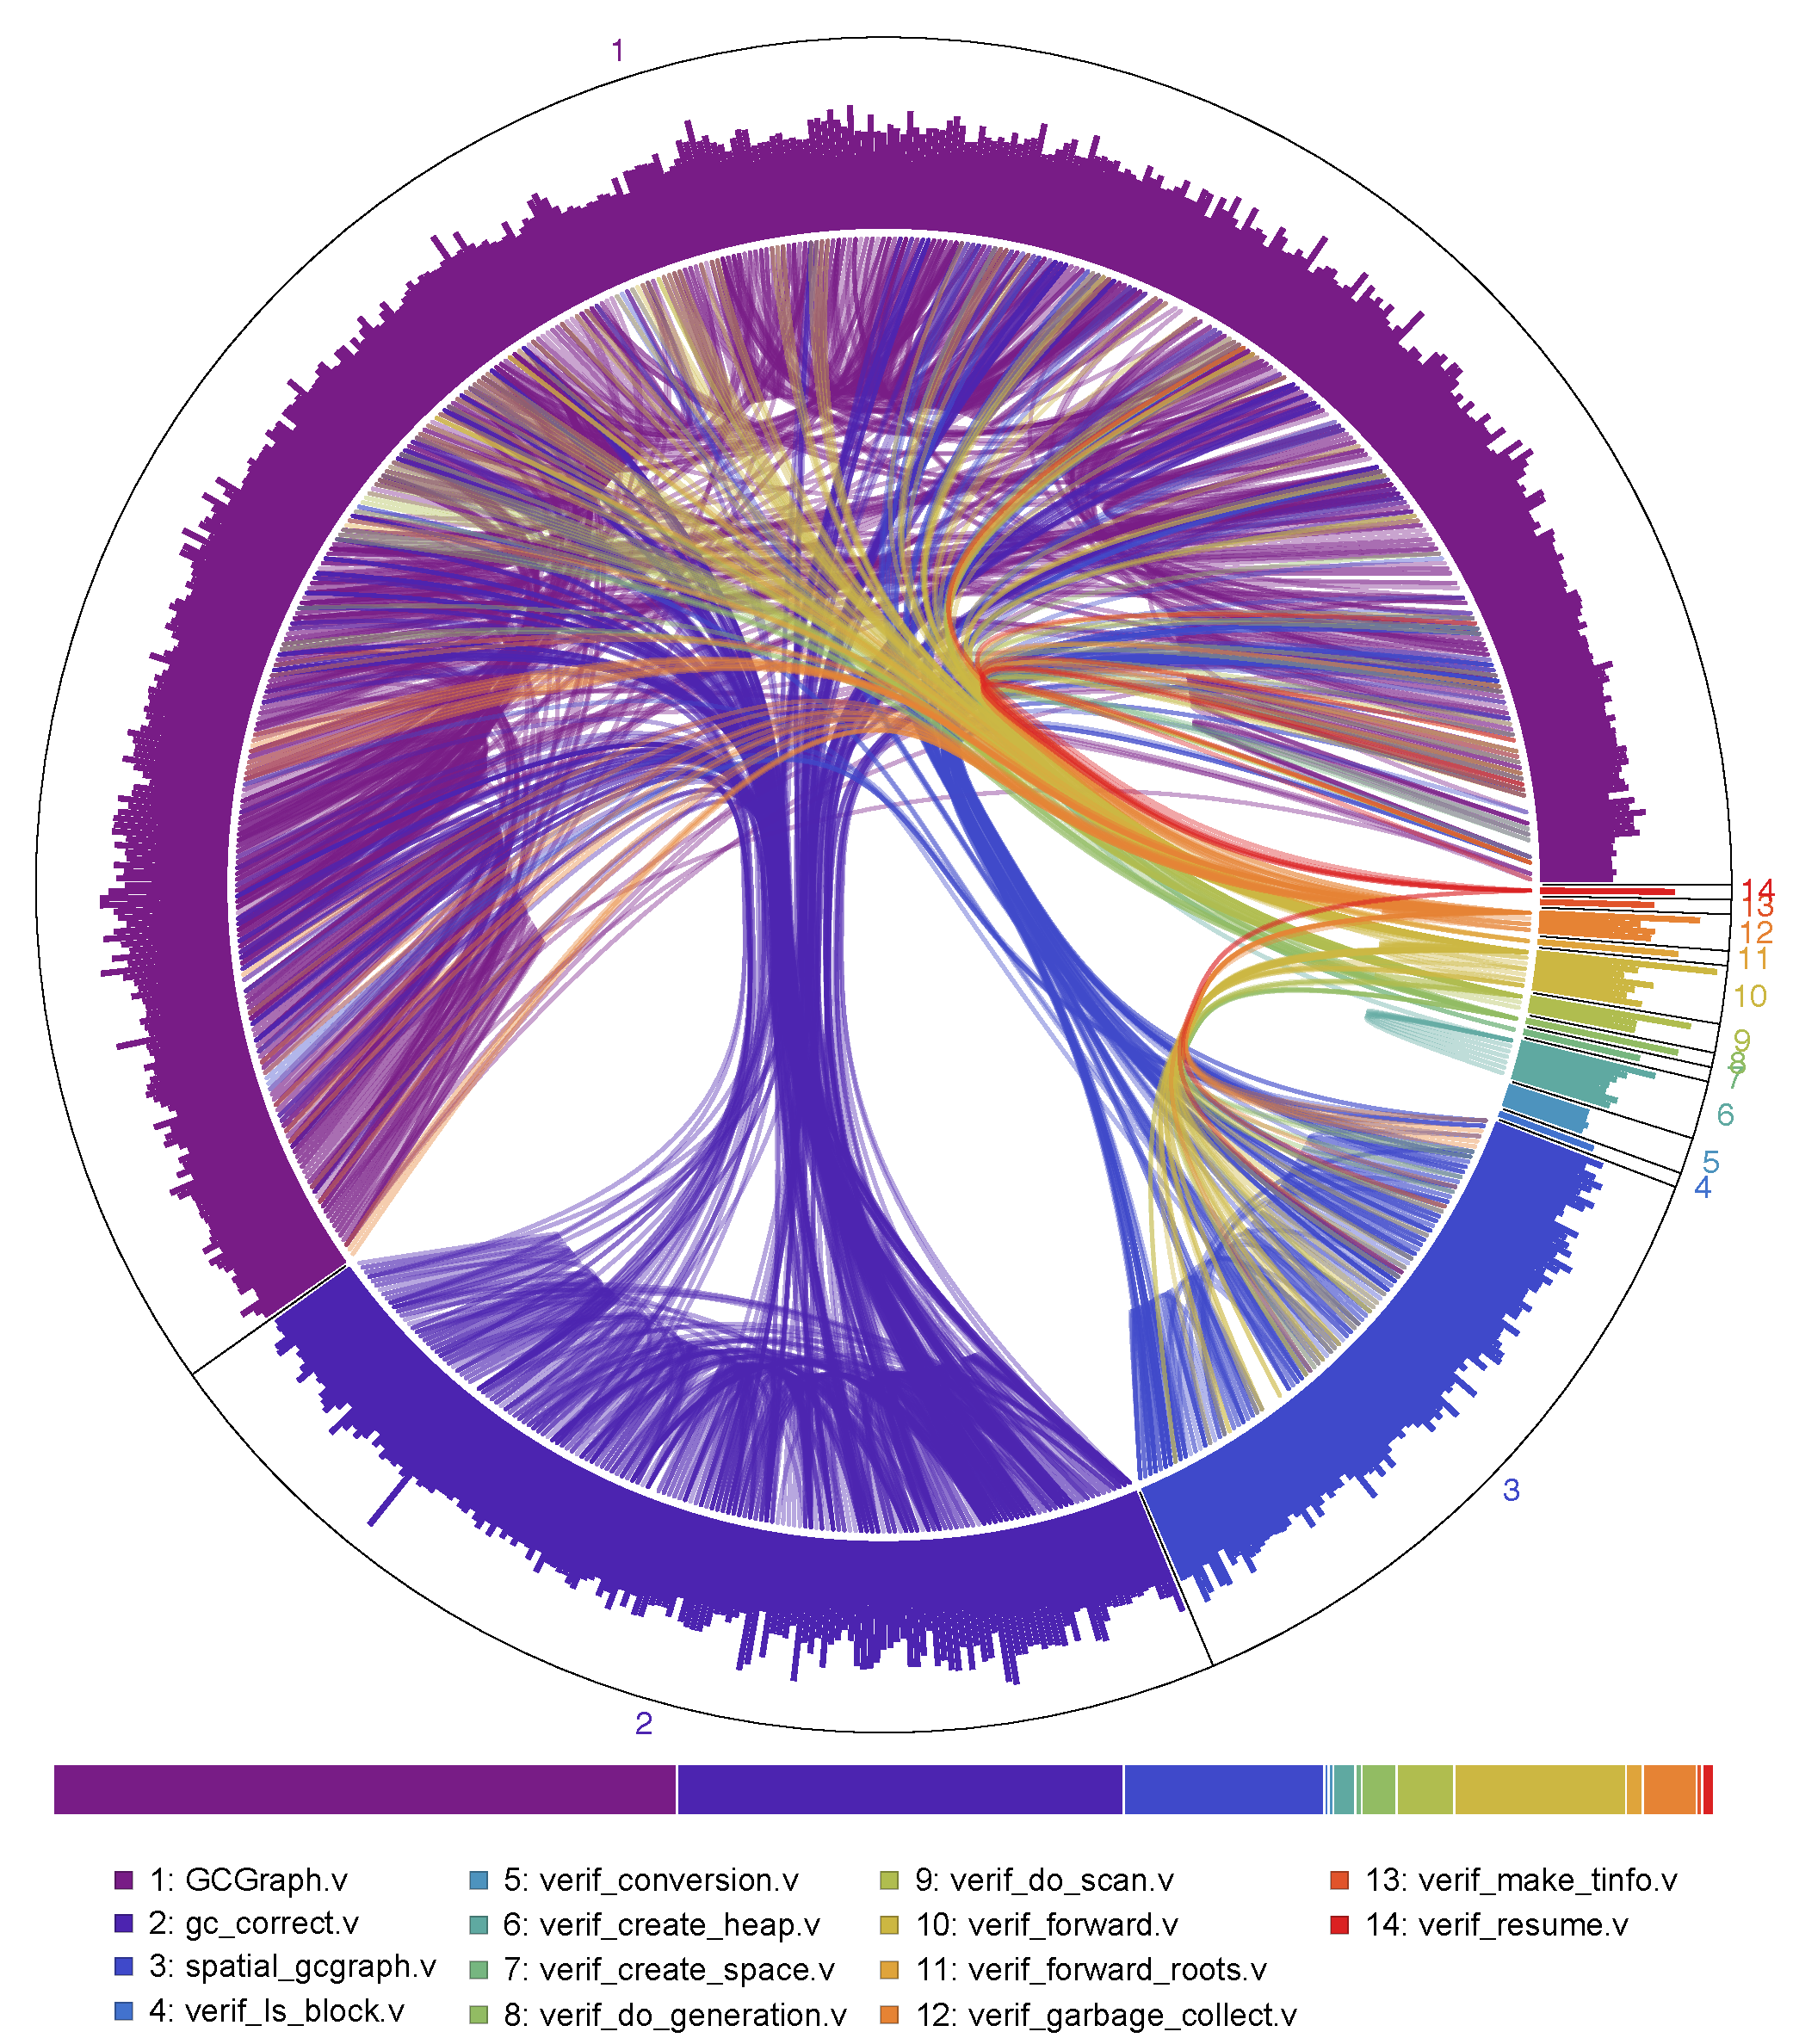
\includegraphics[width=0.95\textwidth]{certigc_theorems}
\caption{Theorems in the verification of the GC}
\label{fig:connectedness}
\end{figure}

We worked to make our library modular, thus encouraging 
proof reuse. Figure~\ref{fig:connectedness} gives a sense of this 
engineering effort.
$14$ files were used to verify the garbage collector, and
the bar at the bottom shows their relative lengths.
Each straight line in the perimeter represents a theorem used to verify the GC, 
and the length of a line corresponds to the length of the theorem on a 
logarithmic scale. The $14$ color-coded sectors represent the files in which 
these theorems are housed. Arcs connecting theorems represent dependencies, 
where an arc is colored the same as the theorem's \emph{caller}.

Sector $1$ contains $432$ generic helper theorems used to check that functions
satisfy the inductive spatial relations that we need. These theorems do not depend
on any other GC theorems. Sector $3$ contains $91$ theorems that establish  
spatial correctness (see~\S\ref{sec:spacegraph}). Sectors $4$-$14$ are the actual
proof scripts for individual functions of the C code. Unsurprisingly, they depend
chiefly on Sectors $1$ and~$3$. 
Among these, sector $10$ is notably large, and this makes sense given that it houses 
our workhorse \li{forward} function. The C code of \li{forward} is~$35$ lines, 
and its verification is~$1309$ lines long: a~$37$-fold blowup.
Sector $2$ contains $155$ theorems that 
prove the final mathematical graph isomorphism (see~\S\ref{sec:mathgraph}).
These theorems depend only on Sector $1$, 
and no other sectors depend on them. This is to be expected, seeing as graph
isomorphism is our final goal. 

\subsection{Statistics Related to our Development}
\label{sec:stats}

\begin{table}[b]
\centering
\caption{Statistics for our code base}
\begin{tabular}{c|c|c|c|c|c}
Component & Section & Files & Size (in lines) & Definitions & Theorems\\\hline
Common Utilities & & 10 & 3,578 & 44 & 289 \\
Math Graph Library & \S\ref{sec:mathgraph} & 20 & 10,585 & 216 & 581 \\
Spatial Graph Library & \S\ref{sec:spacegraph} & 3 & 2,328 & 59 & 110 \\
Integration into VST & \S\ref{sec:localizations},\S\ref{sec:development} & 11 & 2,783 & 17 & 172 \\
\hline
Marking (graph and DAG) & \S\ref{sec:localizations} & 6 & 775 & 9 & 20 \\
Spanning Tree & \S\ref{sec:localizations} & 5 & 2,723 & 17 & 92 \\
Union-Find (heap and array) & \S\ref{sec:orientation} & 18 & 3,193 & 107 & 135 \\
Garbage Collector & \S\ref{sec:certigc} & 16 & 13,858 & 235 & 712 \\
\hline & & & & & \\
[-2.2em] \\
\hline & & & & & \\
[-1em]
Total Development & & 89 & 39,823 & 704 & 2,111 \\
\end{tabular}
\label{tab:codebase}
\end{table}

All our results in this paper have been machine-checked.
Although the size of a development does not perfectly match that development's 
importance or the difficulty of its implementation, 
we present the size nonetheless in Table~\ref{tab:codebase}.
Our proof script is written in a very
dense style.
For comparison, verifying a simple 39-line list-based merge sort in VST takes 600 lines.
At $\approx400$ LOC, the garbage collector is much larger, and is very complicated both
mathematically and spatially, in many places teetering on the edge of what can be defined
in~C. For context, CompCert has 217k LOC, 5,687 definitions, and 6,694 theorems;
VST has 623k LOC, 14,038 definitions, and 21,442 theorems. It is hard to determine
the time taken for this project on the whole, but the verification of the garbage collector
took us eight months.






\hide{
\paragraph{Size of Coq mathgraph \S\ref{sec:mathgraph}.}
Graph folder has 18 files in total with 10,919 lines in total

\paragraph{Size of Coq spacegraph \S\ref{sec:spacegraph}.}

not including the connection to H/S or VST

include \li{Graph.v} and \li{GraphBi.v} from \li{msl_application} since they do not depend on the underlying VST model?

What is in \li{ramification_lemmas}?  
\paragraph{Integration into Floyd (\S\ref{sec:vst}).}: ?
Size of additions to VST logic model: ?

\paragraph{Modifications to HIP/SLEEK.}
H/S code: approximately 2,500 lines of code across 51 files
Size of extra H/S memory model:
\li{alg_seplog_direct.v}  52 lines
\li{overlapping_direct.v} 442 lines  {\color{magenta}How do we handle alignment?}
\li{precise_direct.v} 111 lines
other files?

\paragraph{Size of VST examples~\S\ref{sec:application}.}

Note: graph, graphbi (in space), graphmark, graphbimark are shared in \li{msl_application}

mark graph  19 + 402 + 161 + 246 = 828
mark dag  19 + 402 + 161 + 210
Note: mark dag shares 19 + 402 + 161 with mark graph

copy   459 + 19 + 161 + 388 = 1,027 (need to add files from \li{msl_applicatin})
dispose   475 + 18 + 544 = 1,037 (need to add files from \li{data_structure})
What do copy or dispose share with mark or with each other?

total: 1,038 (marks) + 2,064 (copy/dispose, assuming no duplication) = 3,102 lines.  12 files, assuming no sharing for copy/dispose (with each other or with mark)

\paragraph{Size of H/S example.}
main file: 54 lines (Figure~\ref{fig:hipmarkgraph}), \li{Module Type} generated by H/S (Figure~\ref{fig:hipcoqfile}) is 30 lines, Coq \li{Module} matching this \li{Module Type} is 358 lines.
total: 2 human-generated files, 429 lines

\paragraph{Size of total development.} ?
}
 
\section{Related work}
\label{sec:related}
\paragraph{Comparison with~\citet{hobor:ramification}.}
Our work builds on the theory of ramification by Hobor and Villard,
who verified graph algorithms on pen-and-paper using their \infrulestyle{Ramify} rule:
\begin{equation*}
\inferrule[Ramify]
{\{ L_1 \} ~ c ~ \{ L_2 \} \\
G_1 |- L_1 * (L_2 --* G_2)}
{\{ G_1 \} ~ c ~ \{ G_2 \}} \qquad \mathit{freevars}(L_2 --* G_2) \cap \MV(c) = \emptyset
\end{equation*}
Our \textsc{Localize} rule upgrades \textsc{Ramify} to better handle modified program
variables (note the side condition and recall the discussion in \S\ref{sec:localizations})
and existential quantifiers in postconditions.  Hobor and Villard avoided these challenges
by proposing a unwieldy variant of \infrulestyle{Ramify} called \infrulestyle{RamifyAssign}, which
could reason about the special case of a single assignment $\li{x=}f(\ldots)$, assuming
the verifier can make the local program translation to $\li{x'=}f(\ldots)\li{; x=x'}$,
where \li{x'} is fresh.  This is nontrivial in large existing formal
developments, such as VST, that do not have any way to prove programs equivalent.
Hobor and Villard could not verify unmodified program code, modify program variables
inside nested localization blocks, or handle multiple assignments in a single block as
in lines~\ref{code:markbeforetripleramify}--\ref{code:markaftertripleramify} of
Figure~\ref{fig:markgraph}.  They avoided existentials in localized
postconditions by defining all mathematical operations (\emph{e.g.} $\m{mark}$) as
functions rather than as relations; this is fine for pen-and-paper, but painful in
a mechanized setting wherein functions must be proven to terminate.

Hobor and Villard treated mathematical graphs as triples $(V,E,L)$ of
vertices, edges, and a vertex labeling function, where vertices had no more than two
neighbors. Our mathematical graph framework~(\S\ref{sec:mathgraph}) is more
modular and versatile, and ships with hundreds of reusable definitions and theorems. Further, our library has been tuned to work smoothly in a mechanized context.


Hobor and Villard erroneously defined spatial graphs
recursively. Unfortunately, other members of the research
community (\emph{e.g.}~\citet{raadvg15}) followed their lead.  We expose this
error~(\S\ref{sec:fixpointfail}) and provide a sound and rather general definition for
\p{graph} that recovers fold/unfold reasoning~(\S\ref{sec:goodgraph}).  We develop a
much more general and more modular set of related lemmas and connected our spatial
reasoning to the verification framework of CompCert/VST~(\S\ref{sec:vst}).
Our development is entirely
machine-checked~(\S\ref{sec:development}) whereas they used only pen and paper.

\paragraph{Other Pen-and-Paper Verification of Graph Algorithms and/or $**$.}

\citet{hongseok:phd} verified the Schorr-Waite algorithm, and this 
is widely considered a landmark in the early separation logic literature. 
\citet{bornat:aliasing04}~gave an early attempt to reason about graph algorithms 
in separation logic in a more general way. 
\citet{neelthesis}~provided the first separation logic proof of union-find.

\citet{rey-slnotes}~was the first to document the overlapping 
conjunction $**$, albeit without any strategy to reason about it using Hoare rules. 
\citet{gardnerms12}~were the first to reason about a program using $**$ in 
Javascript. 
\citet{raadvg15}~used $**$ within their CoLoSL program logic to reason about 
a concurrent spanning algorithm using a kind of ``concurrent localization''.



\paragraph{Machine-Checked Verification of Graph Algorithms.}
A decade after Yang verified Schorr-Waite on paper, \citet{leino10} automated 
its verification in Dafny. 
\citet{ilya-graphs}~verified a concurrent spanning tree algorithm, and 
moreover developed mechanized Coq proofs. Their algorithm was written in FCSL, 
a monadic DSL that combines effectful operations with pure Coq expressions; 
FSCL cannot be executed. 
\citet{chen18}~compared how three provers (Coq, Isabelle, and Why3) can 
verify Tarjan’s strongly-connected component algorithm written in the native 
language of each of the tools. Because these are written in the native languages 
of a proof assistant, they avoid “real-world” language concerns such as 
memory models and overflow.

\citet{lamneu15}~extended the Isabelle Refinement Framework to verify a range of 
DFS algorithms via stepwise refinement.
Their framework allows the reuse of previously-proved DFS 
invariants by establishing an inductive
``most specific invariant'' and deriving other inductive invariants from it.
\citet{lamsef19}~extended this further and presented verifications of 
the correctness and time complexity of the Edmonds-Karp and push-relabel
algorithms. Lammich et al. produced very readable proofs of classic 
textbook algorithms by using the Isar language atop their Isabelle proofs.
They used Isabelle's code generator to export efficient executable code, 
but with the caveat that the code comes with a guarantee of only 
partial correctness semantics.

\citet{char11}~used his CFML tool to Coq-verify an OCaml implementation of 
Dijkstra. 
\citet{gueneauetal19}~extended CFML and verified the correctness 
and time complexity of a modified version of the BFGT cycle-detection algorithm.
The graph algorithms verified in CFML tend to be ``graph theory'' in flavour, 
whereas the algorithms we have verified tend to have more of a
``systems'' flavor. This difference is partially explained by the fact that 
code written in ML can take advantage of its high-level design, whereas
code written in C is often interested in handling grungy systems tasks. For 
example, references in ML cannot be null and do not support pointer arithmetic; 
of course both are possible---and lead to nontrivial complications---in 
C. Accordingly, the CFML proofs benefit from ML’s cleaner computational model. 
Our verifications are in C so we must contend with C’s memory model, pointer 
arithmetic, significant scope for undefined behavior, and so forth.

\citet{charpott15, charpott19}~used CFML to verify the correctness and 
time complexity of union-find. Their work is an interesting counterpoint to 
ours because, while it maintains an abstraction between the client and the 
internal mathematical/spatial facts that the client need not know, it does 
not maintain a separation between the mathematical and spatial 
facts themselves, as we do in~\S\ref{sec:mathgraph} and ~\S\ref{sec:spacegraph}.
This separation is worthwhile: our modular method let us verify an alternate 
version of union-find that uses an array of vertices rather than individually 
heap-allocated nodes. This 
secondary verification then used \emph{exactly the same} mathematical proof of 
functional correctness despite the radically different layout of spatial 
memory.
Our work does not verify the time complexity of union-find. When 
we attempted to prove the necessary amortisation bounds we ran into an 
overflow issue: it was impossible to prove that the rank would not exceed 
\li{max\_int} because the CompCert memory model does not place a bound on the 
total number of allocations. Informally, this overflow is impossible in 
practice because no computer has $2^{2^{\tiny 64}}$ bytes of memory, which would 
be required for this overflow to occur, but Coq remains unconvinced. 
Chargu{\'{e}}raud and Pottier acknowledged and sidestepped this issue by 
representing rank using the Coq type \li{Z}, which was not an option for us 
given the end-to-end nature of the VST+CompCert toolchain.

\paragraph{Verification Tools in Coq.}
Our work interacts with the Floyd verification module within the Verified 
Software Toolchain (VST)~\cite{appel:programlogics}. The Floyd module uses 
tactics to enable the separation-logic verification of CompCert C programs. 
VST connects to the CompCert certified C compiler~\cite{leroy:compcert}, and 
thus has no gaps or admits between the verified source code and the eventual
assembly code~\cite{appelvst}.

Charge! likewise uses Coq tactics to work with a shallow embedding of higher 
order separation logic, but focuses on OO programs written in 
Java/C\#~~\cite{bengtson:charge}. Iris Proof Mode provides a similar framework 
for higher-order concurrent reasoning in Coq~\cite{krebbers:iris}.

CFML enables the verification of OCaml programs by reasoning about their
``characteristic formulae'' in separation logic using Coq~\cite{char10, char11}. 
CFML has been used to verify a range of functional and imperative programs,
including some graph-related algorithms as discussed 
above. \citet{charpott15, charpott19}~extended CFML to reason about time 
credits. The work of \citet{gueneau17}~indicates that CFML is exploring a connection 
with the certified CakeML compiler~\cite{cakeml}.

While the tools above require substantial human guidance, 
Bedrock~\cite{chlipala:bedrock} is a more automated approach to the verification of 
low level programs using separation logic in Coq. 
Bedrock leverages the fact that phrasing function 
specifications in a \emph{computational} style 
(in this case, inspired by functional programming) 
leads to separation logic proof obligations that are quite automatable.
It simplifies these obligations into pure mathematics using a 
custom workhorse tactic, and then discharges those 
obligations using standard Coq automation.

\paragraph{Other Verification Tools.} 

Many more-automated verification tools also use separation logic in a forward
reasoning style. Smallfoot~\cite{berdine:smallfoot}, jStar~~\cite{distefanop08}, 
HIP/SLEEK~\cite{chin:hipsleek}, and Verifast~\cite{jacobs:verifast} are landmarks
at various points on the expressibility-automatability spectrum. 
KeY~\cite{beckert:2007} and Dafny~\cite{leino10} are verifiers that are not 
based on separation logic. KeY uses an interactive verifier while Dafny pursues
 automation with Z3~\cite{moura2008}.

\paragraph{Mechanized Mathematical Graph Theory.}
There is a long history, going back at least 28 years, of mechanized 
reasoning about mathematical graphs~\cite{wong1991}. 
The most famous mechanically verified “graph theorem” is the Four Color 
Theorem~\cite{gonthier2005computer}; however the development actually uses
hypermaps instead of graphs. In general most “mathematical graph” frameworks in 
the literature~\cite{wong1991, chou1994, yamamoto1995formalization, rwpgt1998, yamamoto1998formalization, tamai2000formal, duprat2001coq, ridge2005graphs, nipkow2016, dijkstra_shortest_path-afp} were not used to verify real 
code, for which they seem unsuitable. Verifying real code requires delicate concepts such as removing a subgraph, null nodes, and parallel edges, and one of our contributions is that our framework is general enough to support such verification. 
\citet{noschinski2015}~built a graph library in Isabelle/HOL whose formalization 
is the closest to ours, 
\emph{e.g.} supporting graphs with labeled and parallel arcs. 
Beyond being in Coq, our setup supports at least three features beyond 
Noschinski’s: reasoning about incomplete graphs (as discussed 
in~\S\ref{sec:mathinfra} using figure~\ref{fig:pregraph}), labeling the graph 
as a whole (used, for example, in the garbage collector to store 
metainformation about the number and location of the generations), and our 
modular typeclass-supported “graphs with properties” setup in General Graph 
(as described in~\S\ref{subsec:graphplugins}). 
\citet{dubois2015graphes} and \citet{noschinski2015formalizing}~used proof assistants to 
design verifiable checkers for solutions to graph problems. 
\citet{bauer20025} and \citet{yamamoto1995formalization}~used an inductive encoding of graphs to formalize planar graph theory.


\paragraph{Verification of Garbage Collection Algorithms.}
Schism \cite{gcexample4,gcexample4a} is a certified concurrent
collector built in a Java VM that services multi-core architectures with weak memory consistency.
\citet{gcexample5, gcexample3} introduced GCminor, which is
a certified translation step added to CompCert's translation from Clight to assembly.
GCminor makes explicit the specific invariants that the garbage collector
relies upon, thus minimising errors due to the violation of invariants
between the garbage collector and the mutator.
\citet{gcexample2} annotated x86 code
for two GCs by hand, and then used Boogie and the Z3 automated theorem prover
to verify their correctness automatically.

The closest piece of work to our certified GC is probably the excellent certified GC
for the Cake ML project~\cite{cakemlgc}, since both integrate a certified GC into 
a certified compiler for a functional language.  Their GC is written closer to assembly 
than C, which is both a positive---in that they avoid undefined behaviors---and a negative, 
in that their GC is harder to understand and upgrade and cannot take advantage of the
mature CompCert compiler.  Their GC lacks some of our optimisations (\emph{e.g.} they have 
only three generations), but on the other hand handles mutation in the GC heap.  The largest 
difference, however, is that we present an integrated graph framework suitable for reasoning 
about many graph algorithms, of which our GC is merely the flagship.  In contrast, they focus 
much more narrowly on the problem of certified GCs.
 
\section{Future work and conclusion}
\label{sec:future}
\label{sec:conclusion}
In the future we plan to improve the pure reasoning of graphs and
similar data structures, with a particular focus on automation.  We have
also begun to investigate integrating our techniques into the 
HIP/SLEEK toolchain~\cite{chin:hipsleek}, which, as compared to VST, 
provides more automation at the cost of lower expressivity.  We
are also interested in investigating better ways to handle the
kinds of undefined behavior upon which real~C systems code sometimes
relies.

\hide{\color{magenta}We are in the process of verifying a garbage
collector for the ``CertiCoq'' project, which is building
a certified compiler from Gallina to Clight. We would like to investigate
using our externally verified lemmas in HIP/SLEEK to verify code such as fast
exponentiation and more graph algorithms. We also would like to make
the interface between Coq and H/S simpler and cleaner.
One final direction we would like to investigate is using our new
connection to Coq to have H/S output certificates as it
verifies programs so that the system becomes more trustworthy.}

Our main contributions were as follows.  We developed a mathematical
graph library that was powerful enough to reason about graph-manipulating
algorithms written in real~C code.  We connected these mathematical graphs
to spatial graphs in the heap via separation logic.  We developed 
localization blocks to smoothly reason about a local action's effect on
a global context in a mechanized context, including a robust treatment
of modified program variables and existential quantifiers in postconditions.
We demonstrated our techniques on several nontrivial examples, including union-find
and spanning tree.  Our flagship example was the verification of the garbage collector 
for the CertiCoq project, during which we found two places in which the~C semantics
is too weak to define an OCaml-style GC.  We integrated our techniques into the
VST toolset. 

 
\begin{acks}
We thank Asankhaya Sharma for his help with a previous version of this paper,
Neel Krishnaswami for his helpful suggestions and encouragements, and 
Xavier Leroy and Robbert Krebbers for fruitful discussions. 
We also thank the CertiCoq team (esp. Andrew~W.~Appel, Olivier~Savary~Belanger, and 
Zoe~Paraskevopoulou) for their overall support and for hosting 
Shengyi Wang for a summer. This work was funded in part by the
\grantsponsor{}{Yale-NUS College}{} grant~\mbox{\grantnum{}{R-607-265-322-121}} and the \grantsponsor{}{National Science Foundation}{} grant~\grantnum{}{CCF-1521602}.
Any opinions, findings, and conclusions or recommendations expressed in 
this material are those of the authors and do not necessarily reflect the 
views of Yale-NUS College or the National Science Foundation.
\hide{

This material is based upon work supported by the
  \grantsponsor{GS100000001}{National Science
    Foundation}{http://dx.doi.org/10.13039/100000001} under Grant
  No.~\grantnum{GS100000001}{nnnnnnn} and Grant
  No.~\grantnum{GS100000001}{mmmmmmm}.  Any opinions, findings, and
  conclusions or recommendations expressed in this material are those
  of the author and do not necessarily reflect the views of the
  National Science Foundation.}
\end{acks}

\pagebreak
\bibliography{autoquack}




\end{document}
